%%____________________________________________________________________________||
\section{Results}
\label{sec:results}

In this section the main results concerning the fit are summarised. 

Table ~\ref{} summarises the predicted and observed yields in the signal region, which correspond to an integrated luminosity of 1.28 \ifb. 
The predicted yields are based on a fit to multiple data control samples to obtain predictions in (\nj,\nb,\scalht). 
The observed counts in the signal region are not considered in this fit. 
The uncertainties reflect all statistical and (pre-fit) systematic sources added in quadrature. 
The $\ttbar$W and \znunu components are also shown (the former of which contains all residual contributions from sub-dominant processes such as e.g. diboson production). 
This table summarises our best knowledge of the SM background rates in the signal region while not considering counts in the signal region itself. 

Tables~\ref{tab:yieldsnodata_sig_comb_sym} summarises the predicted and
observed yields in the signal region corresponding to an integrated
luminosity of 1.28 \ifb. The predicted yields are based on a fit to
multiple data control samples to obtain predictions in
(\njet,~\nb,~\scalht). The observed counts in the signal region are
not considered in this fit. The uncertainties reflect all statistical
and (pre-fit) systematic sources added in quadrature. The $\ttbar$W
and \znunu components are also shown (the former of which contains
all residual contributions from sub-dominant processes such as \eg
diboson production). This table summarises our best knowledge of the
SM background rates in the signal region while not considering counts
in the signal region itself.


%% In Figure ~\ref{fig:postFitSummary} the results of the background-only fit for all the analysis bins (\nj,\nb,\scalht) are visually summarised in one single plot, inclusively in the \MHT dimension.

In Figures ~\ref{fig:postFitShapes_eq0b_eq2a}-~\ref{fig:postFitShapes_ge3b_ge5j} the fit in the \MHT dimension is shown for all the analysis bins where the \MHT templates are used.

In Figures ~\ref{fig:nuisPull_alphaT_sym}-~\ref{fig:nuisPull_extrap_asym} the pull of the nuisance parameters with respect to the pre-fit value is shown, 
grouped into different type of nuisances and split between ``asymmetric'' and ``symmetric'' topologies.

%% In Figures ~\ref{fig:postFitShapes_eq0b_eq2j} the fit in the \MHT dimension is shown for all the analysis bins where the \MHT templates are used.


\newpage
\begin{figure}[h!]
\caption{Post-fit \MHT templates for the bin $\nj^{\mathrm{asym}}=2$, $\nb=0$ \label{fig:postFitShapes_eq0b_eq2a}}.
\begin{center}

    \subfigure[$\nj^{\mathrm{asym}}=2$, $\nb=0$, $200 < \scalht < 250 \; \mathrm{GeV}$]{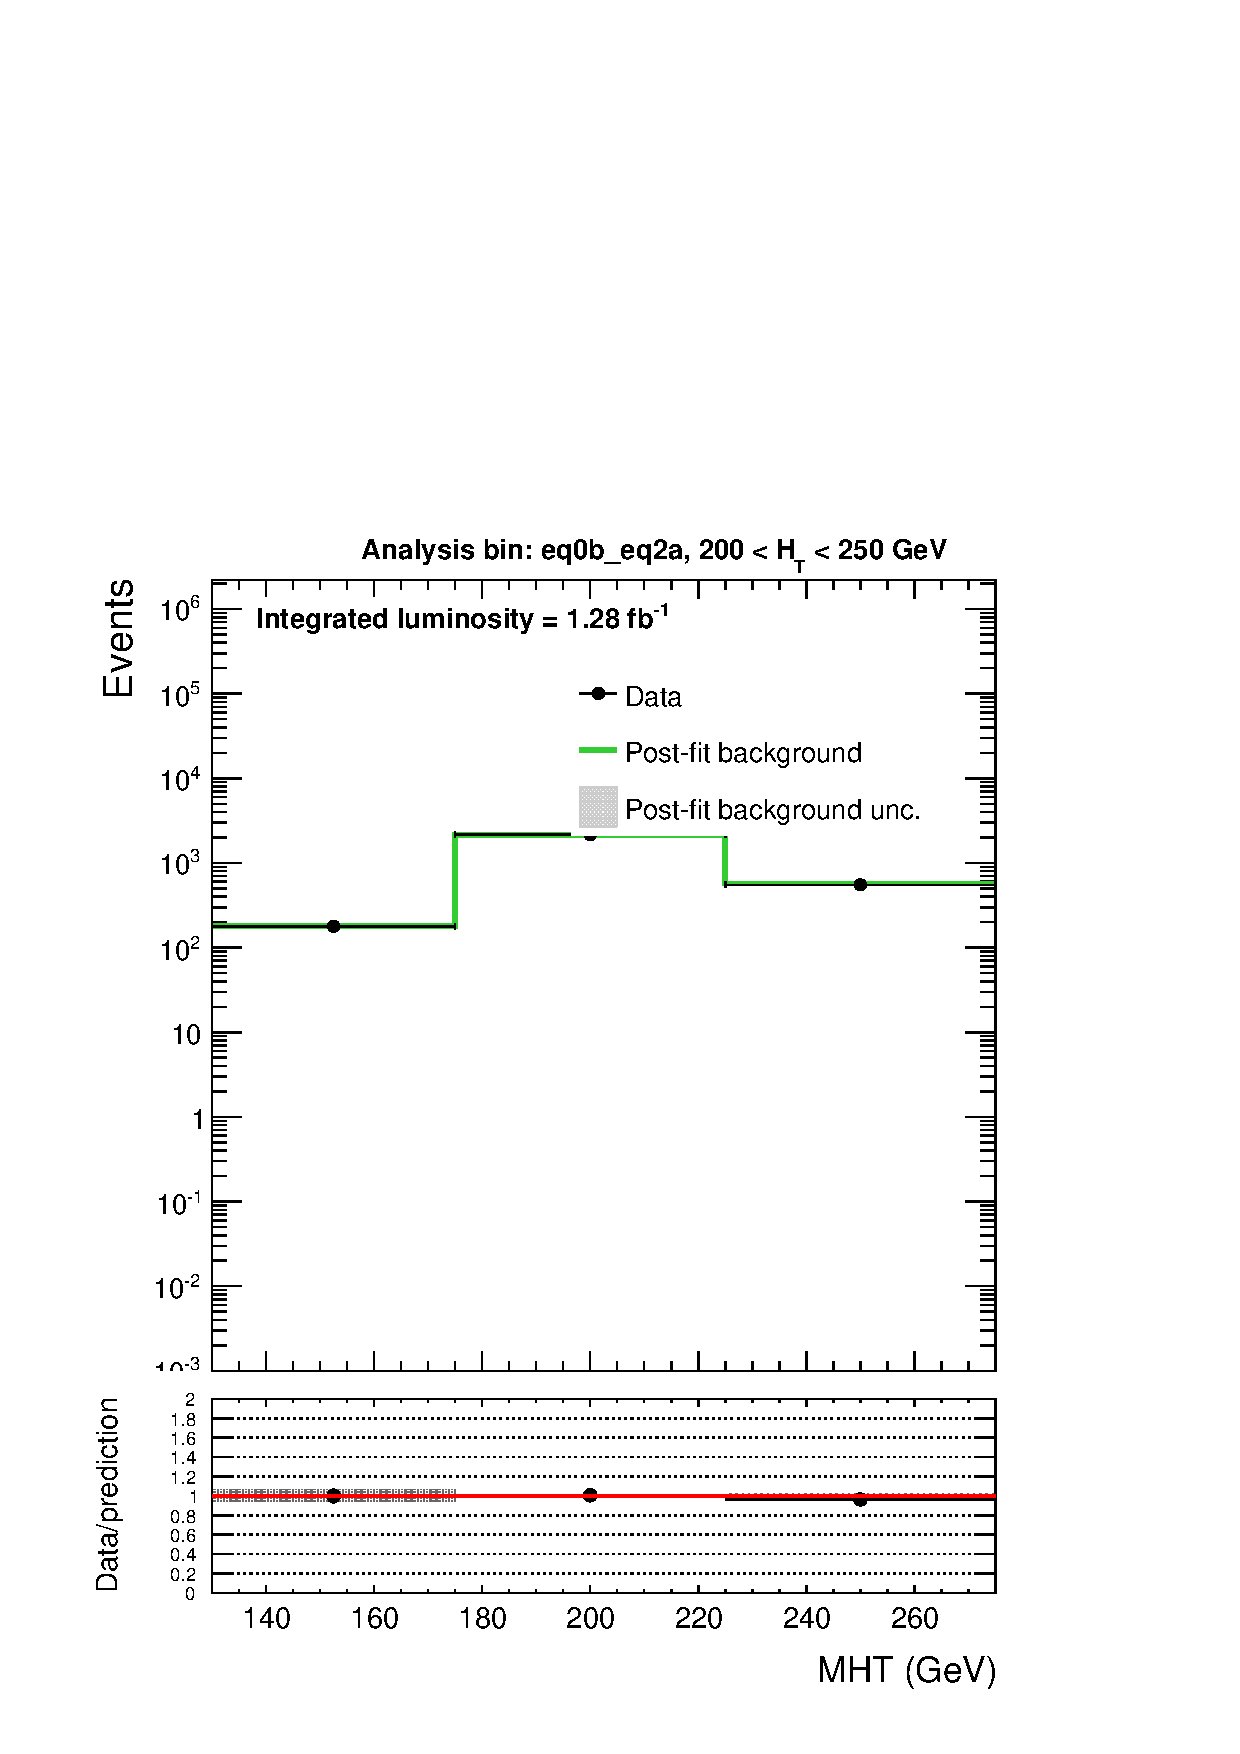
\includegraphics[width=0.25\textwidth]{figures/postFitResults/postFitShape_eq0b_eq2a_200_250.pdf} }\hspace{1cm}
    \subfigure[$\nj^{\mathrm{asym}}=2$, $\nb=0$, $250 < \scalht < 300 \; \mathrm{GeV}$]{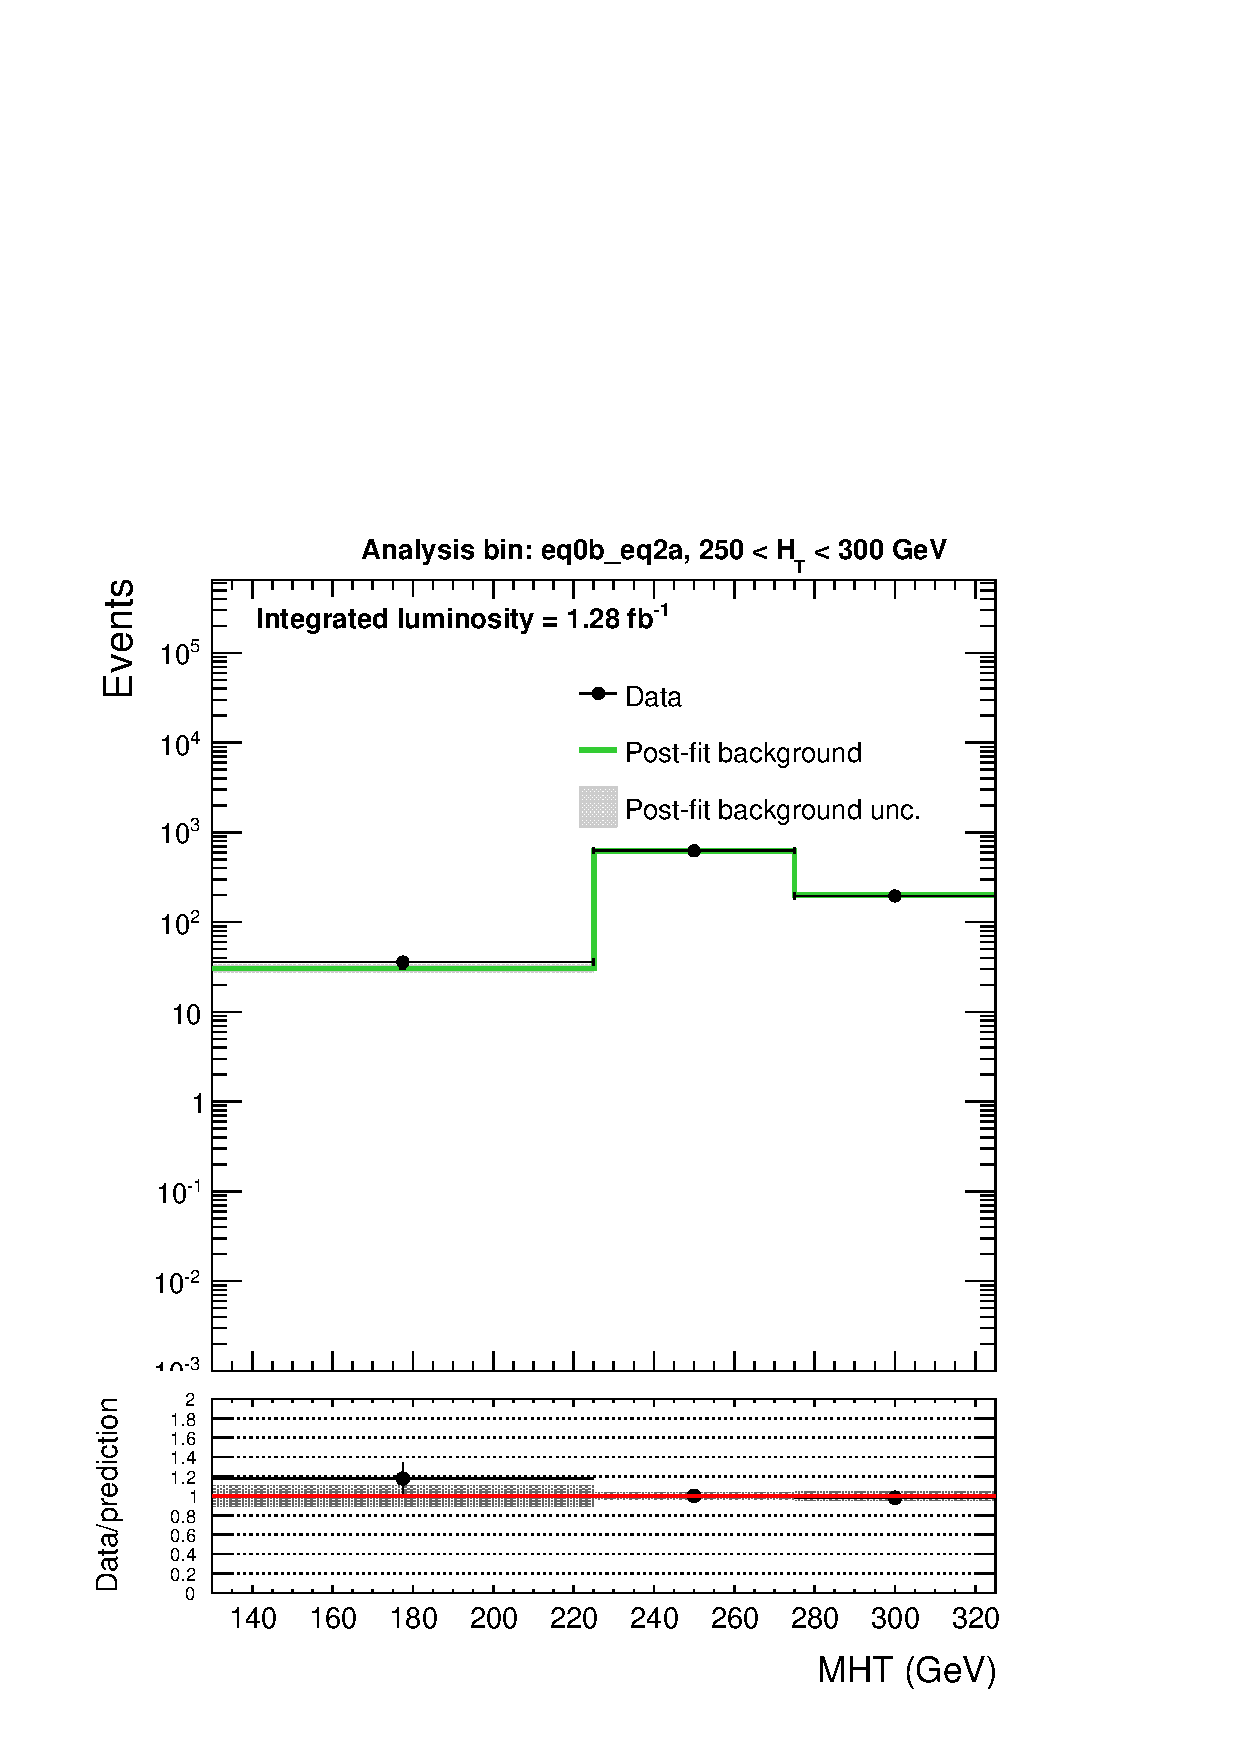
\includegraphics[width=0.25\textwidth]{figures/postFitResults/postFitShape_eq0b_eq2a_250_300.pdf} }\hspace{1cm}
    \subfigure[$\nj^{\mathrm{asym}}=2$, $\nb=0$, $300 < \scalht < 350 \; \mathrm{GeV}$]{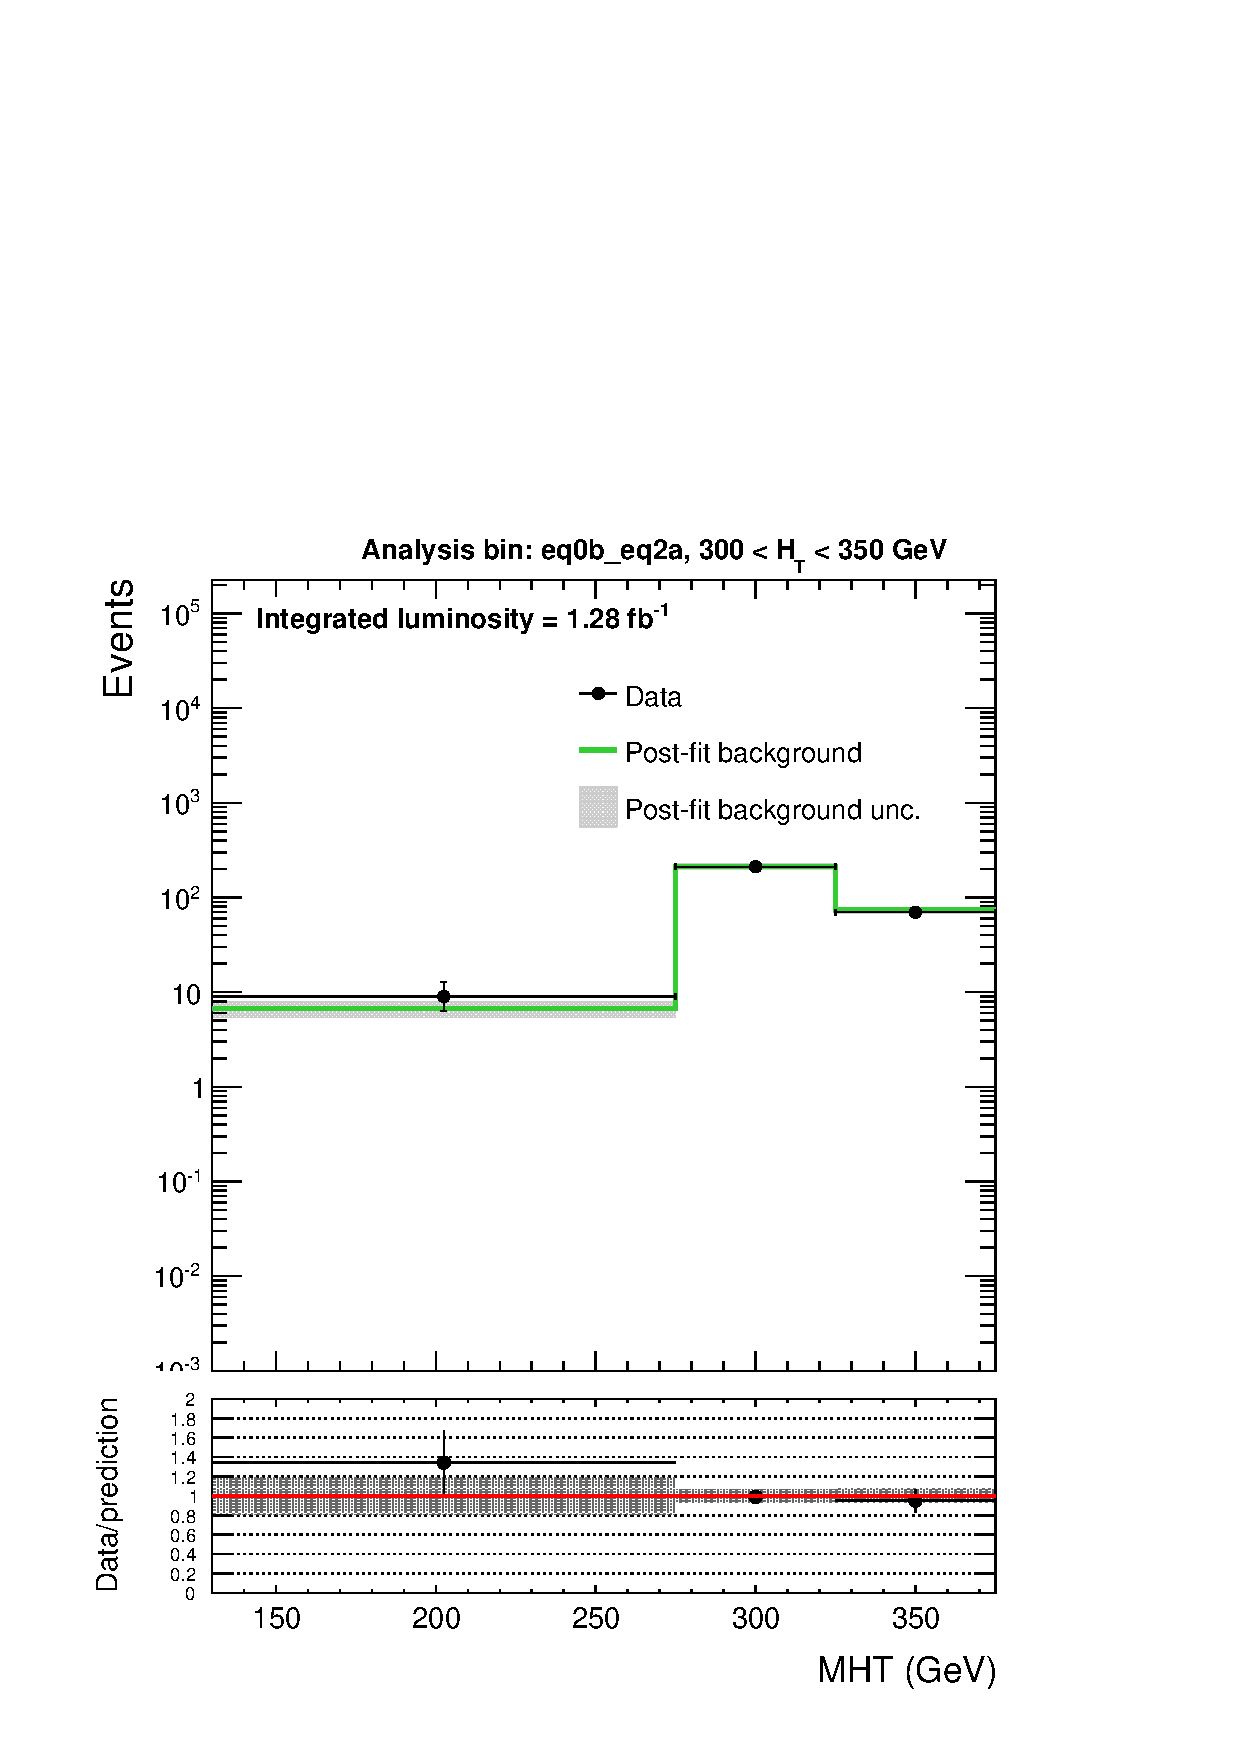
\includegraphics[width=0.25\textwidth]{figures/postFitResults/postFitShape_eq0b_eq2a_300_350.pdf} }\\
    \subfigure[$\nj^{\mathrm{asym}}=2$, $\nb=0$, $350 < \scalht < 400 \; \mathrm{GeV}$]{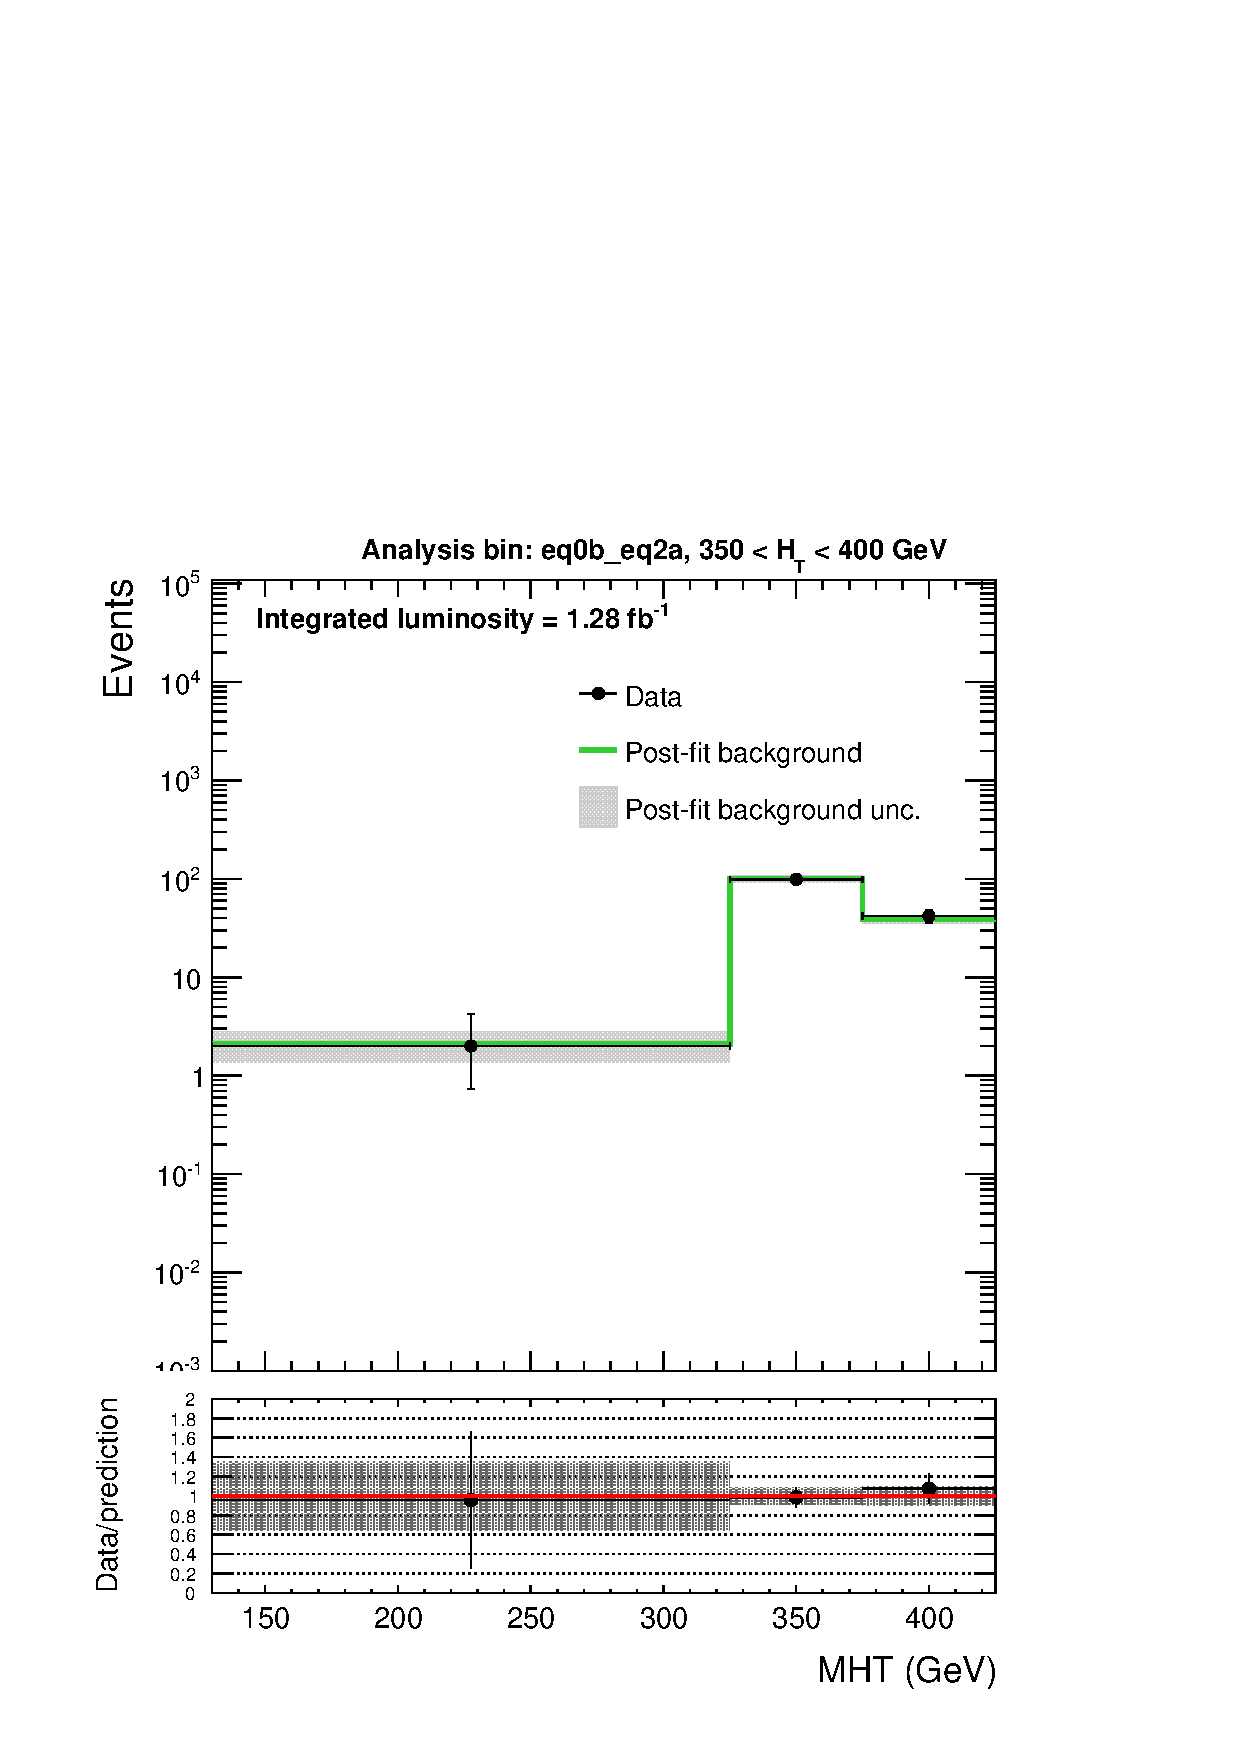
\includegraphics[width=0.25\textwidth]{figures/postFitResults/postFitShape_eq0b_eq2a_350_400.pdf} }\hspace{1cm}
    \subfigure[$\nj^{\mathrm{asym}}=2$, $\nb=0$, $400 < \scalht < 500 \; \mathrm{GeV}$]{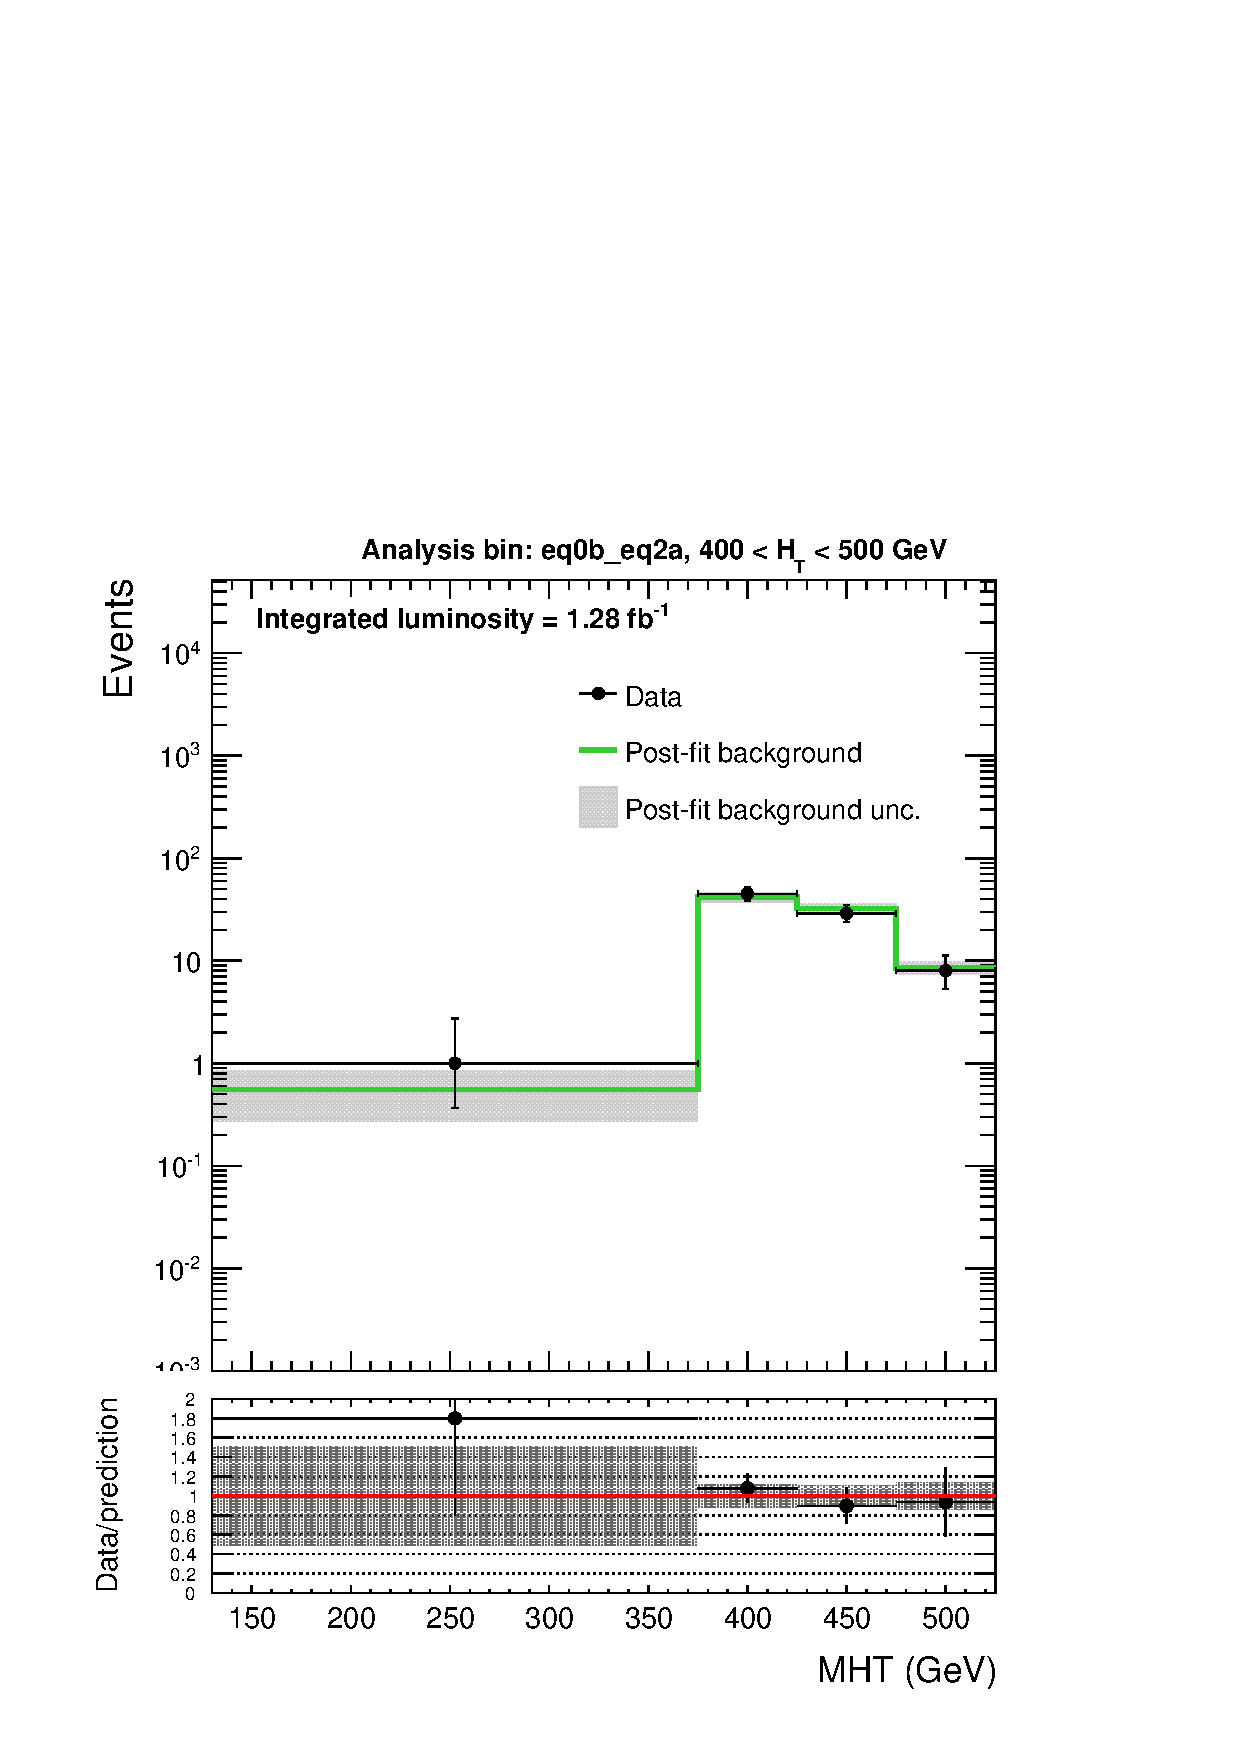
\includegraphics[width=0.25\textwidth]{figures/postFitResults/postFitShape_eq0b_eq2a_400_500.pdf} }\hspace{1cm}
    \subfigure[$\nj^{\mathrm{asym}}=2$, $\nb=0$, $500 < \scalht < 600 \; \mathrm{GeV}$]{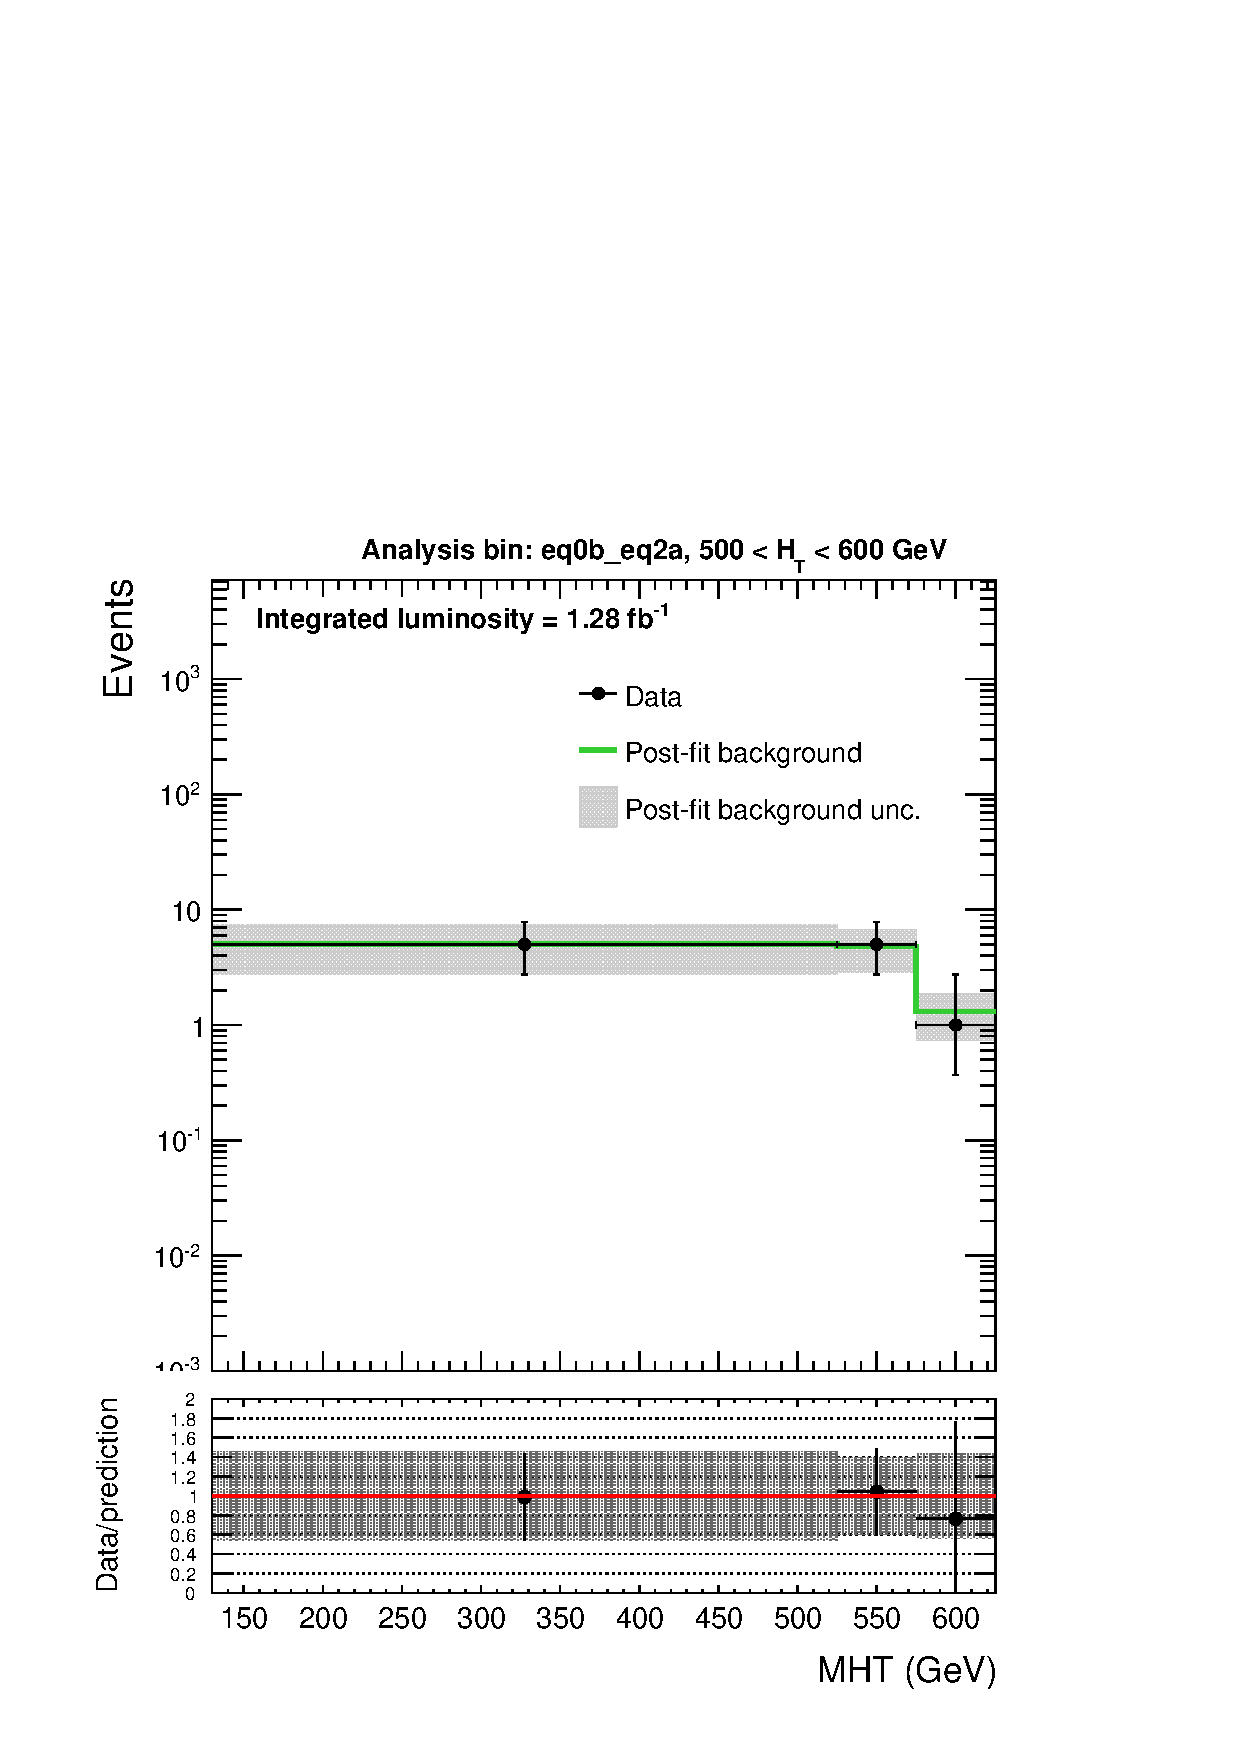
\includegraphics[width=0.25\textwidth]{figures/postFitResults/postFitShape_eq0b_eq2a_500_600.pdf} }\\
    \subfigure[$\nj^{\mathrm{asym}}=2$, $\nb=0$, $\scalht > 600 \; \mathrm{GeV}$]{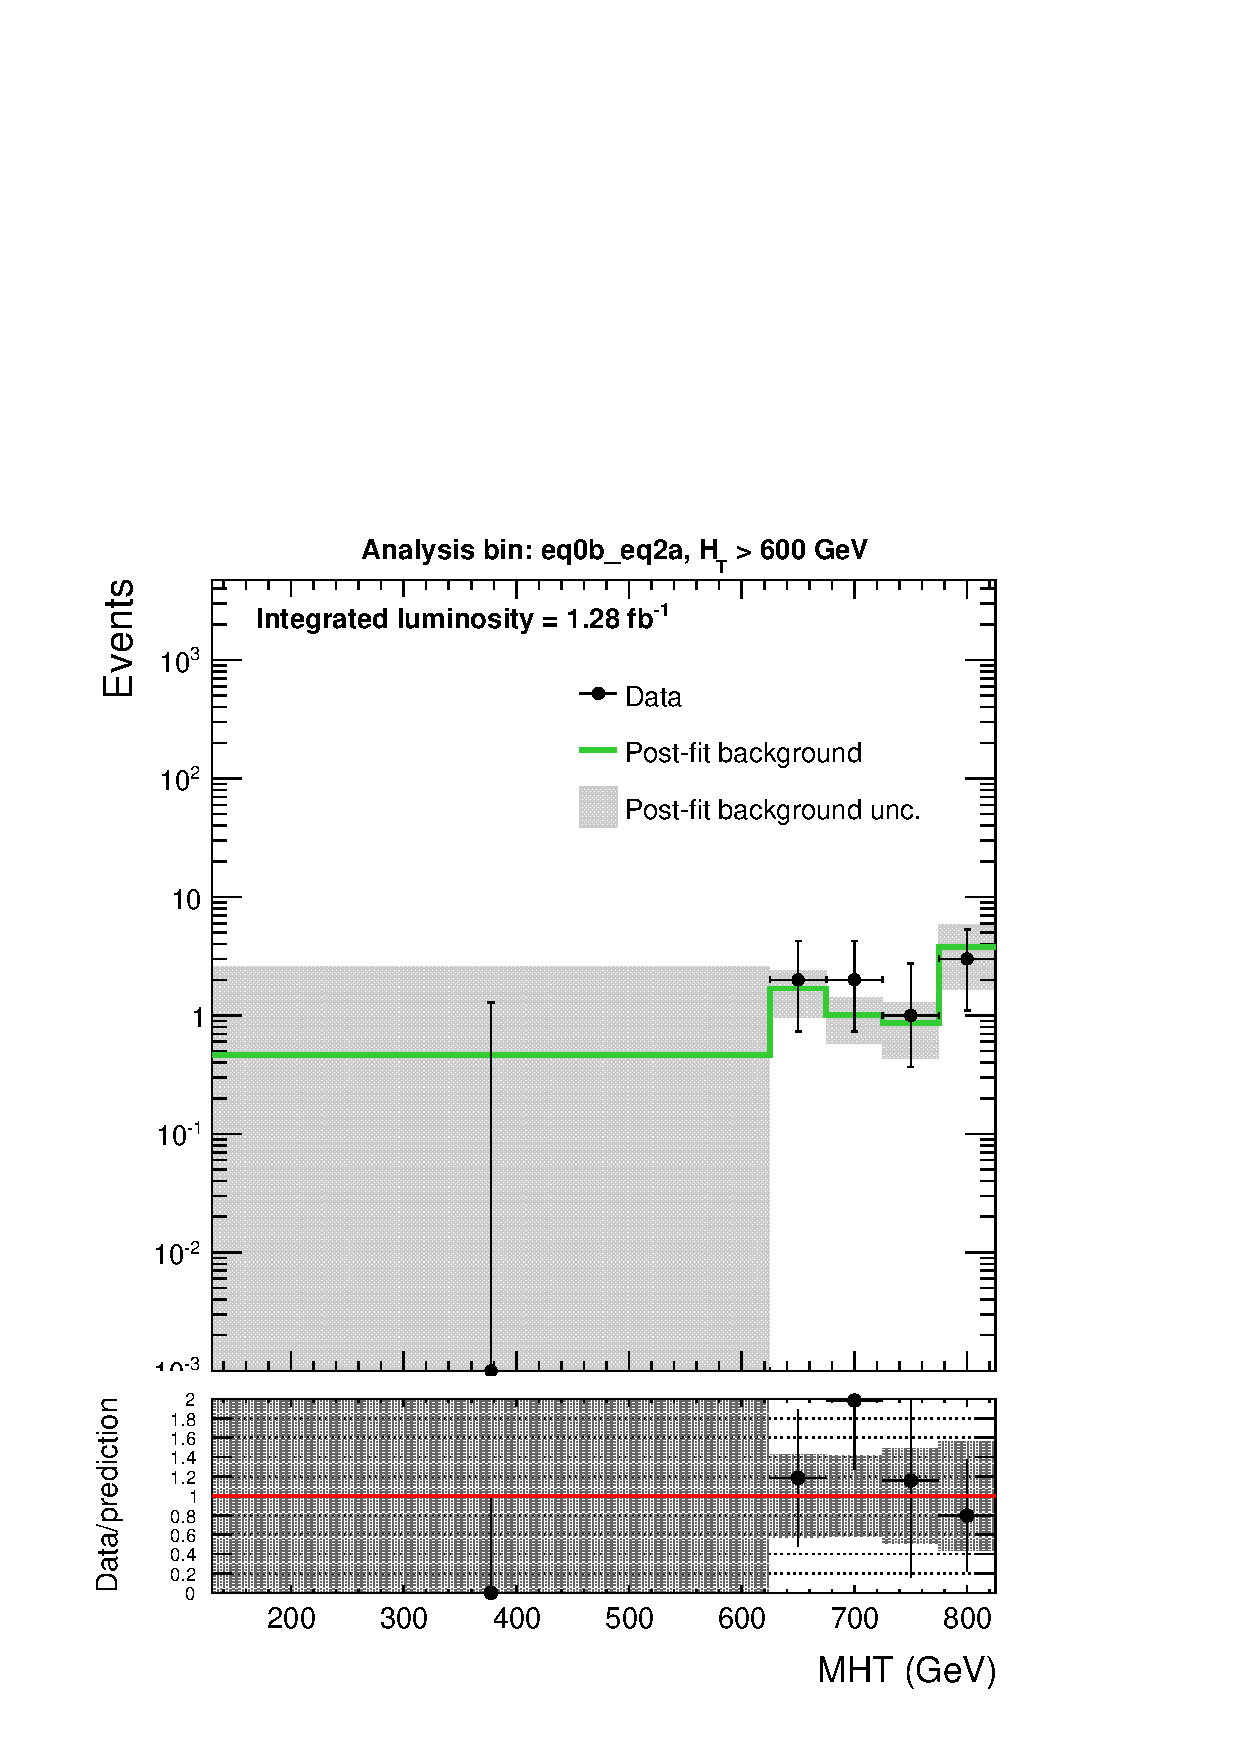
\includegraphics[width=0.25\textwidth]{figures/postFitResults/postFitShape_eq0b_eq2a_600_Inf.pdf} }\hspace{1cm}
  \end{center}
\end{figure}



\newpage
\begin{figure}[h!]
\caption{Post-fit \MHT templates for the bin $\nj^{\mathrm{sym}}=2$, $\nb=0$ \label{fig:postFitShapes_eq0b_eq2j}}.
\begin{center}

    \subfigure[$\nj^{\mathrm{sym}}=2$, $\nb=0$, $200 < \scalht < 250 \; \mathrm{GeV}$]{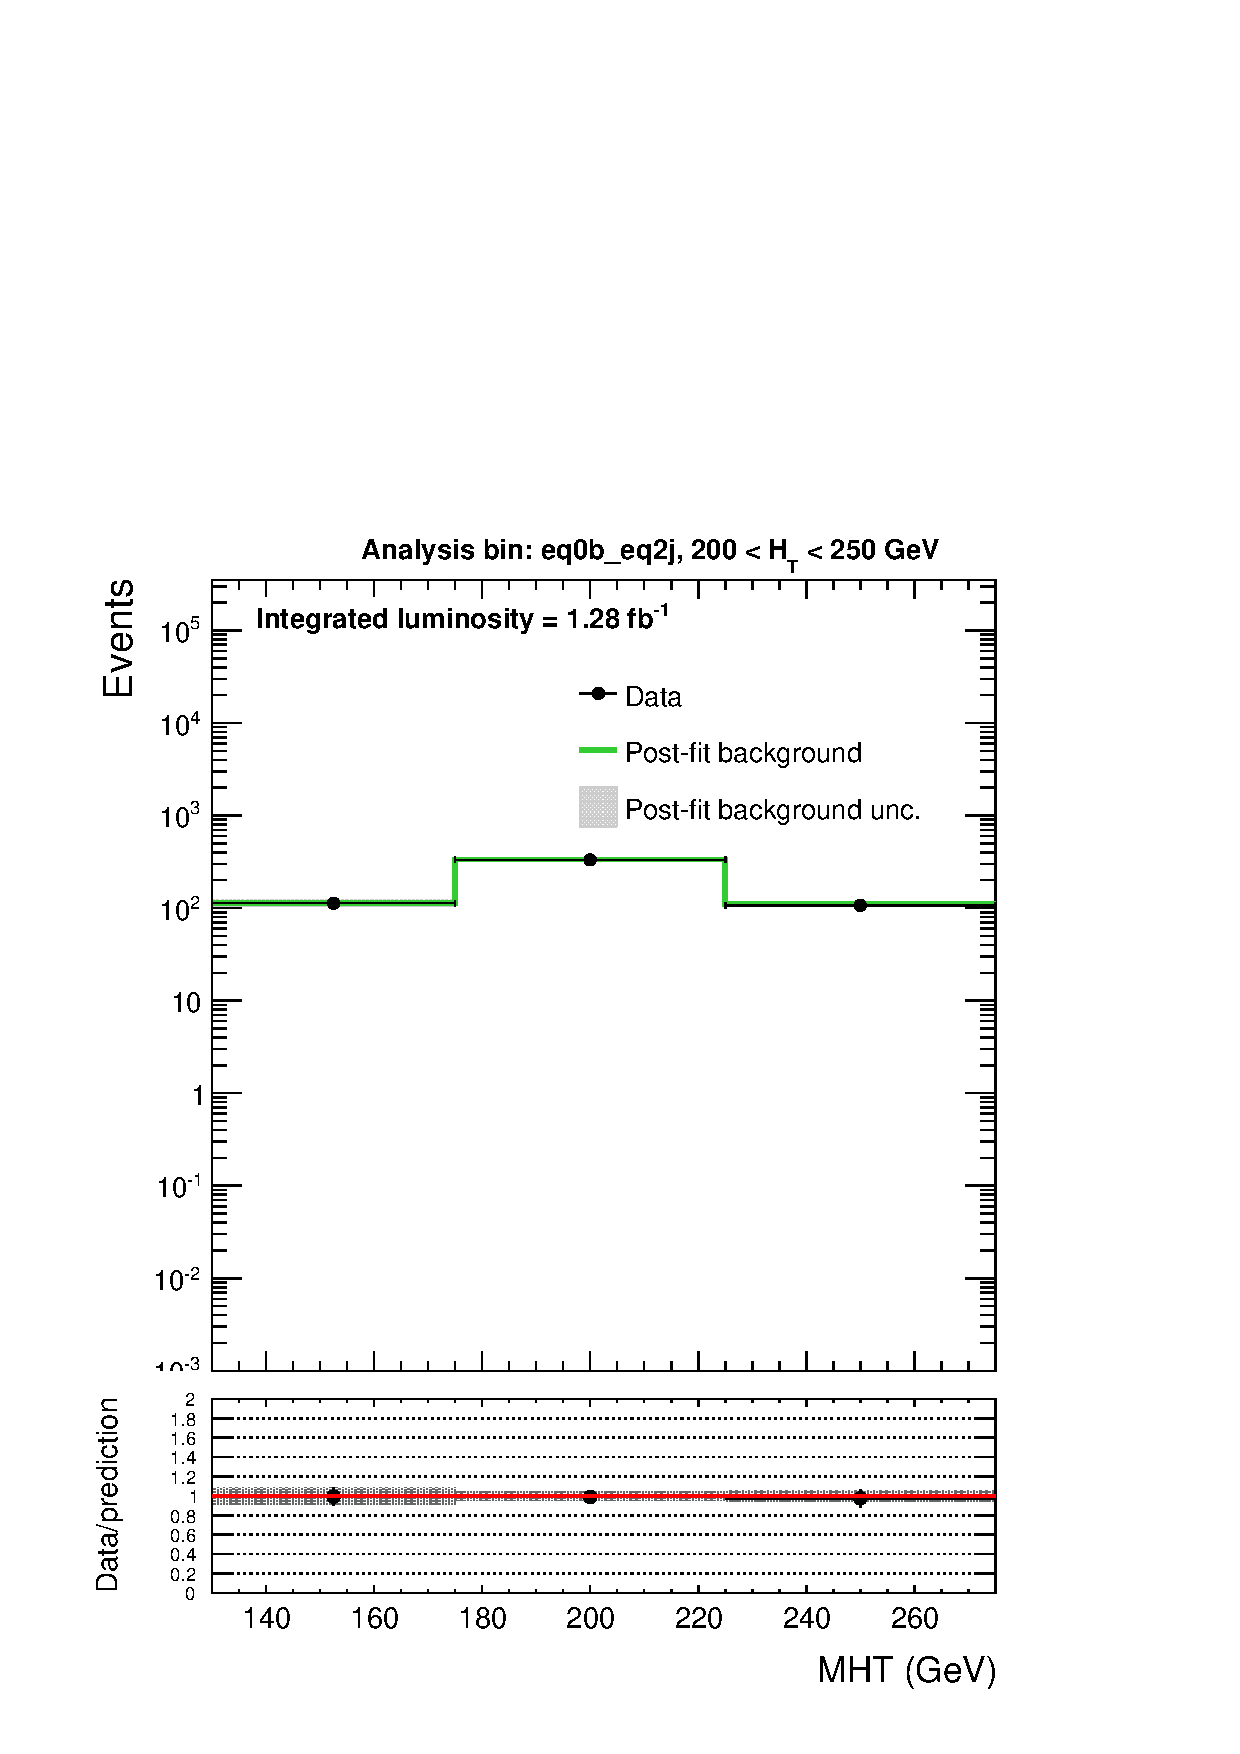
\includegraphics[width=0.25\textwidth]{figures/postFitResults/postFitShape_eq0b_eq2j_200_250.pdf} }\hspace{1cm}
    \subfigure[$\nj^{\mathrm{sym}}=2$, $\nb=0$, $250 < \scalht < 300 \; \mathrm{GeV}$]{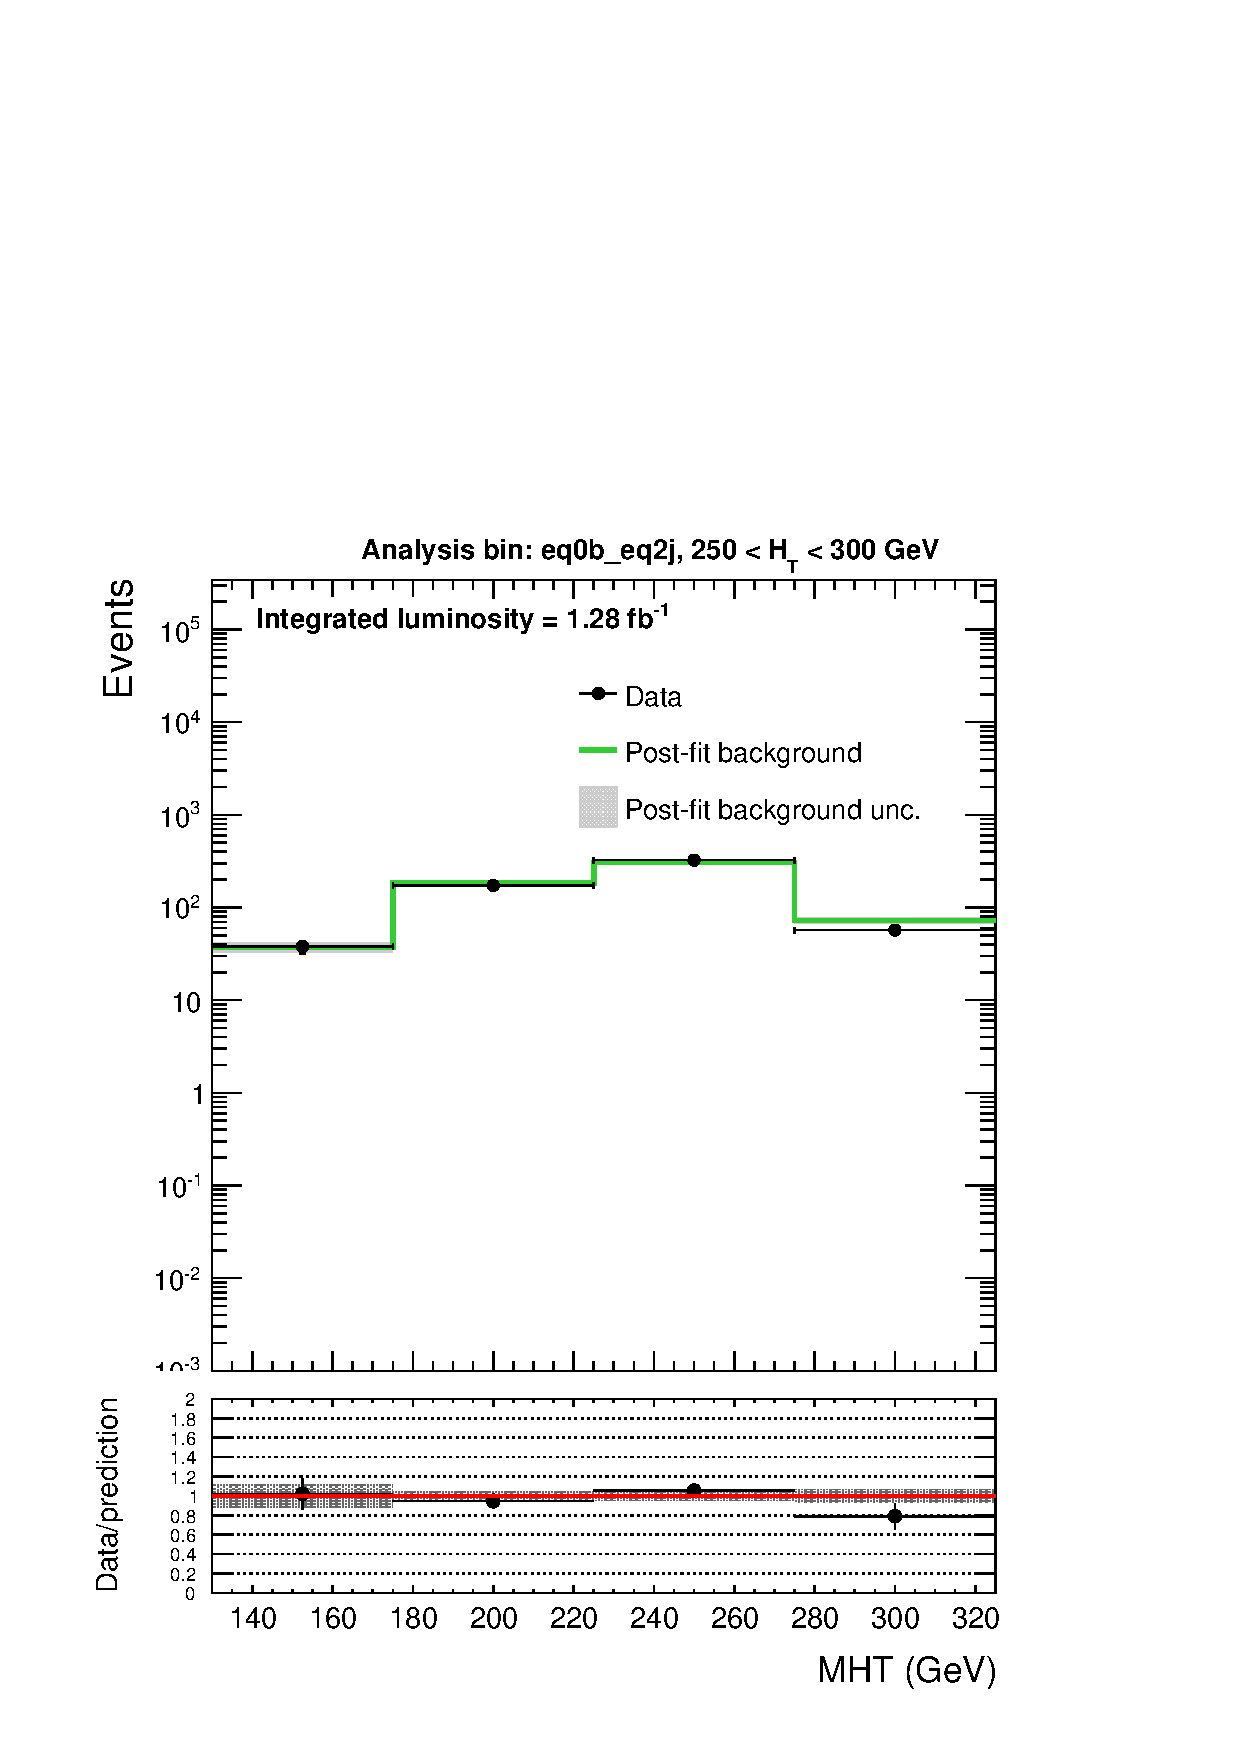
\includegraphics[width=0.25\textwidth]{figures/postFitResults/postFitShape_eq0b_eq2j_250_300.pdf} }\hspace{1cm}
    \subfigure[$\nj^{\mathrm{sym}}=2$, $\nb=0$, $300 < \scalht < 350 \; \mathrm{GeV}$]{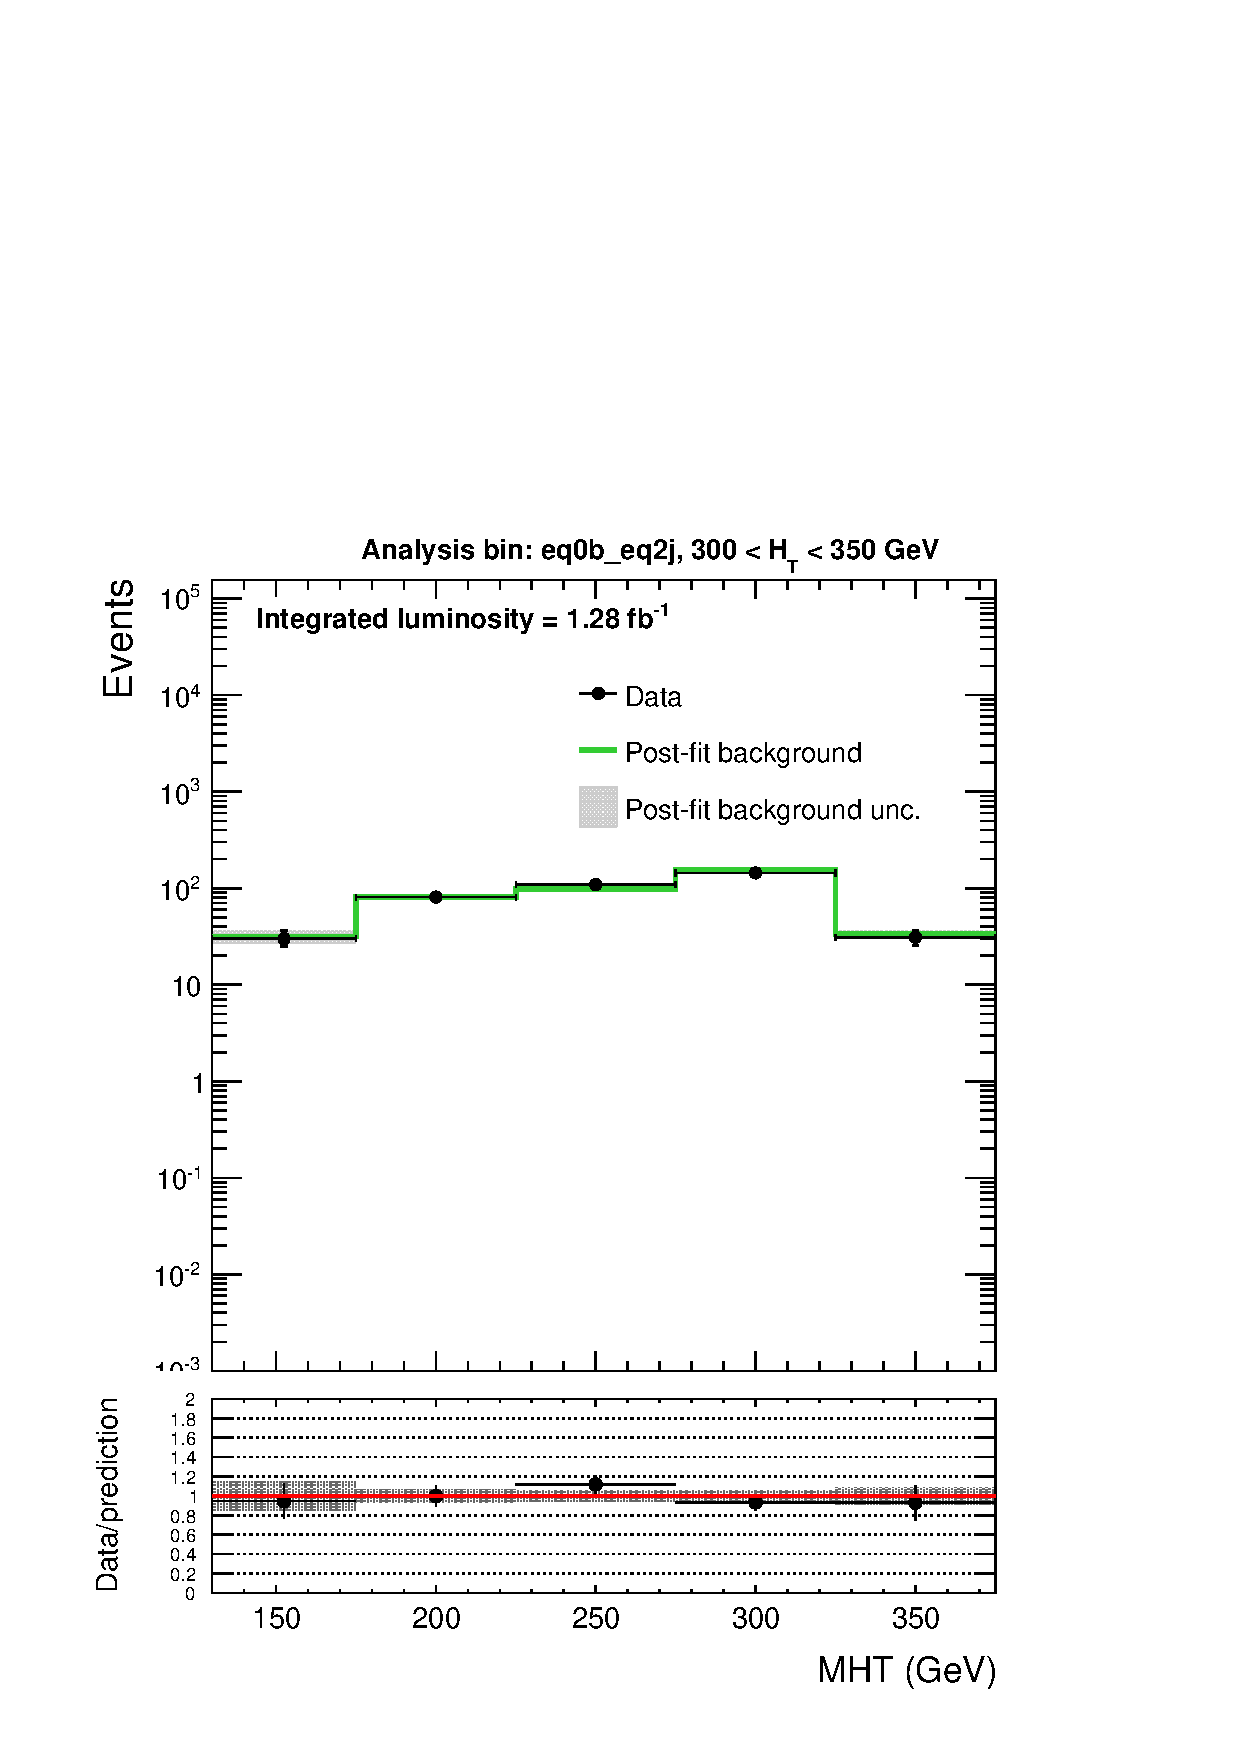
\includegraphics[width=0.25\textwidth]{figures/postFitResults/postFitShape_eq0b_eq2j_300_350.pdf} }\\
    \subfigure[$\nj^{\mathrm{sym}}=2$, $\nb=0$, $350 < \scalht < 400 \; \mathrm{GeV}$]{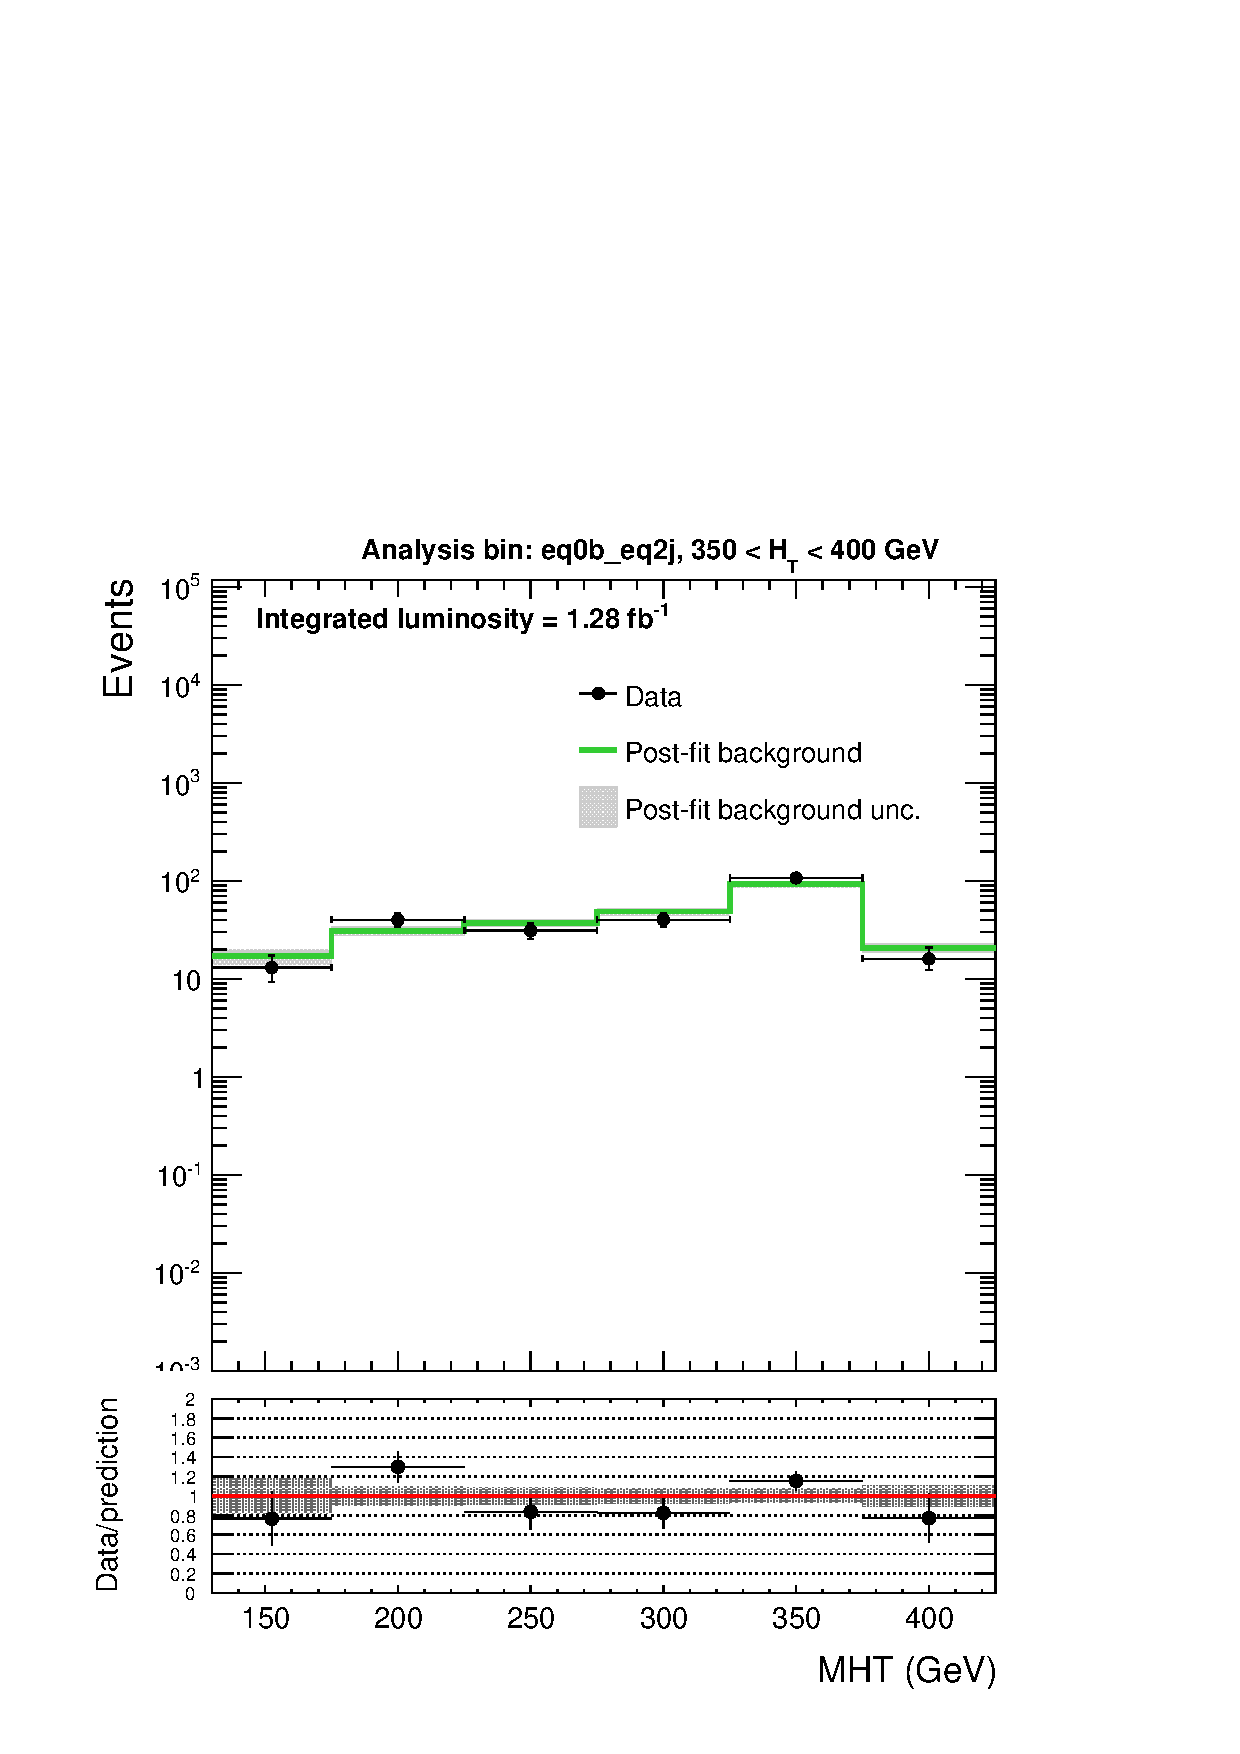
\includegraphics[width=0.25\textwidth]{figures/postFitResults/postFitShape_eq0b_eq2j_350_400.pdf} }\hspace{1cm}
    \subfigure[$\nj^{\mathrm{sym}}=2$, $\nb=0$, $400 < \scalht < 500 \; \mathrm{GeV}$]{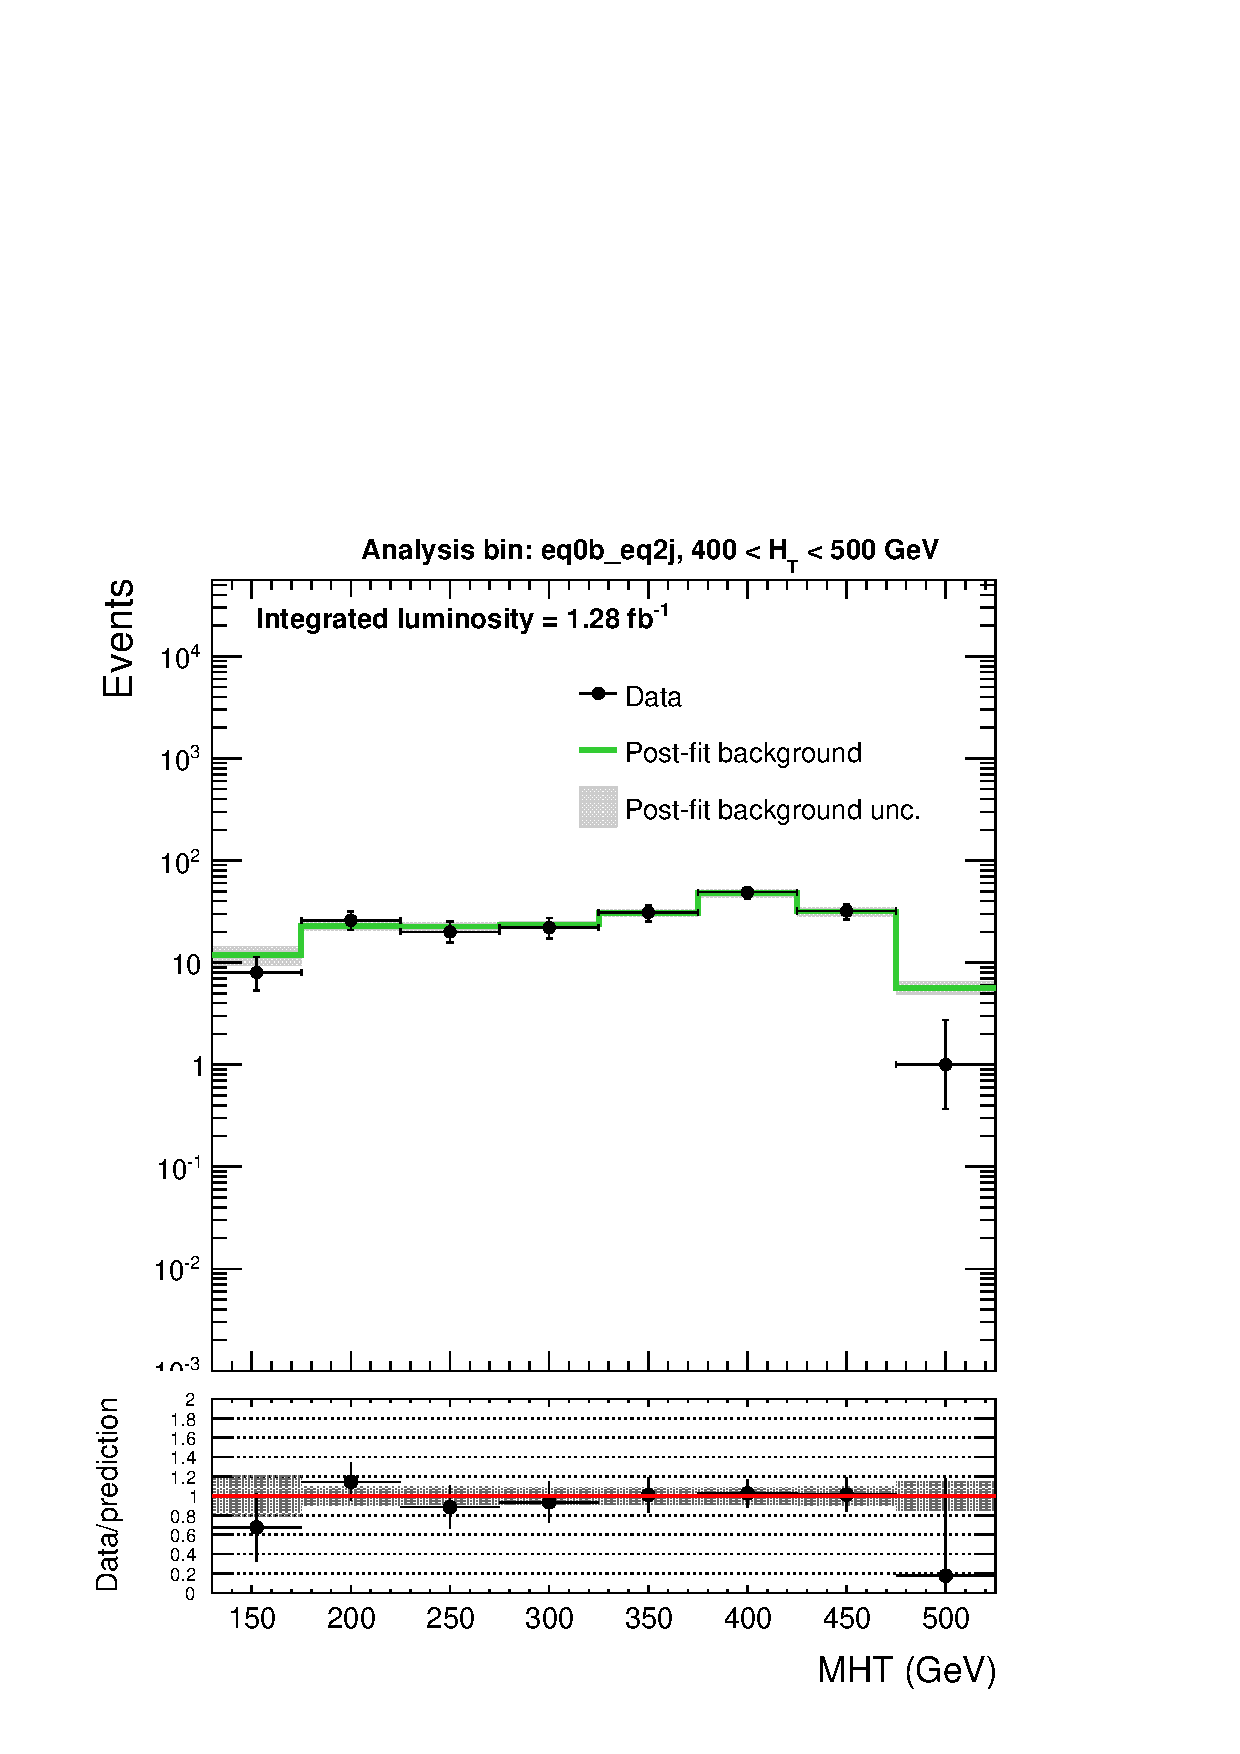
\includegraphics[width=0.25\textwidth]{figures/postFitResults/postFitShape_eq0b_eq2j_400_500.pdf} }\hspace{1cm}
    \subfigure[$\nj^{\mathrm{sym}}=2$, $\nb=0$, $500 < \scalht < 600 \; \mathrm{GeV}$]{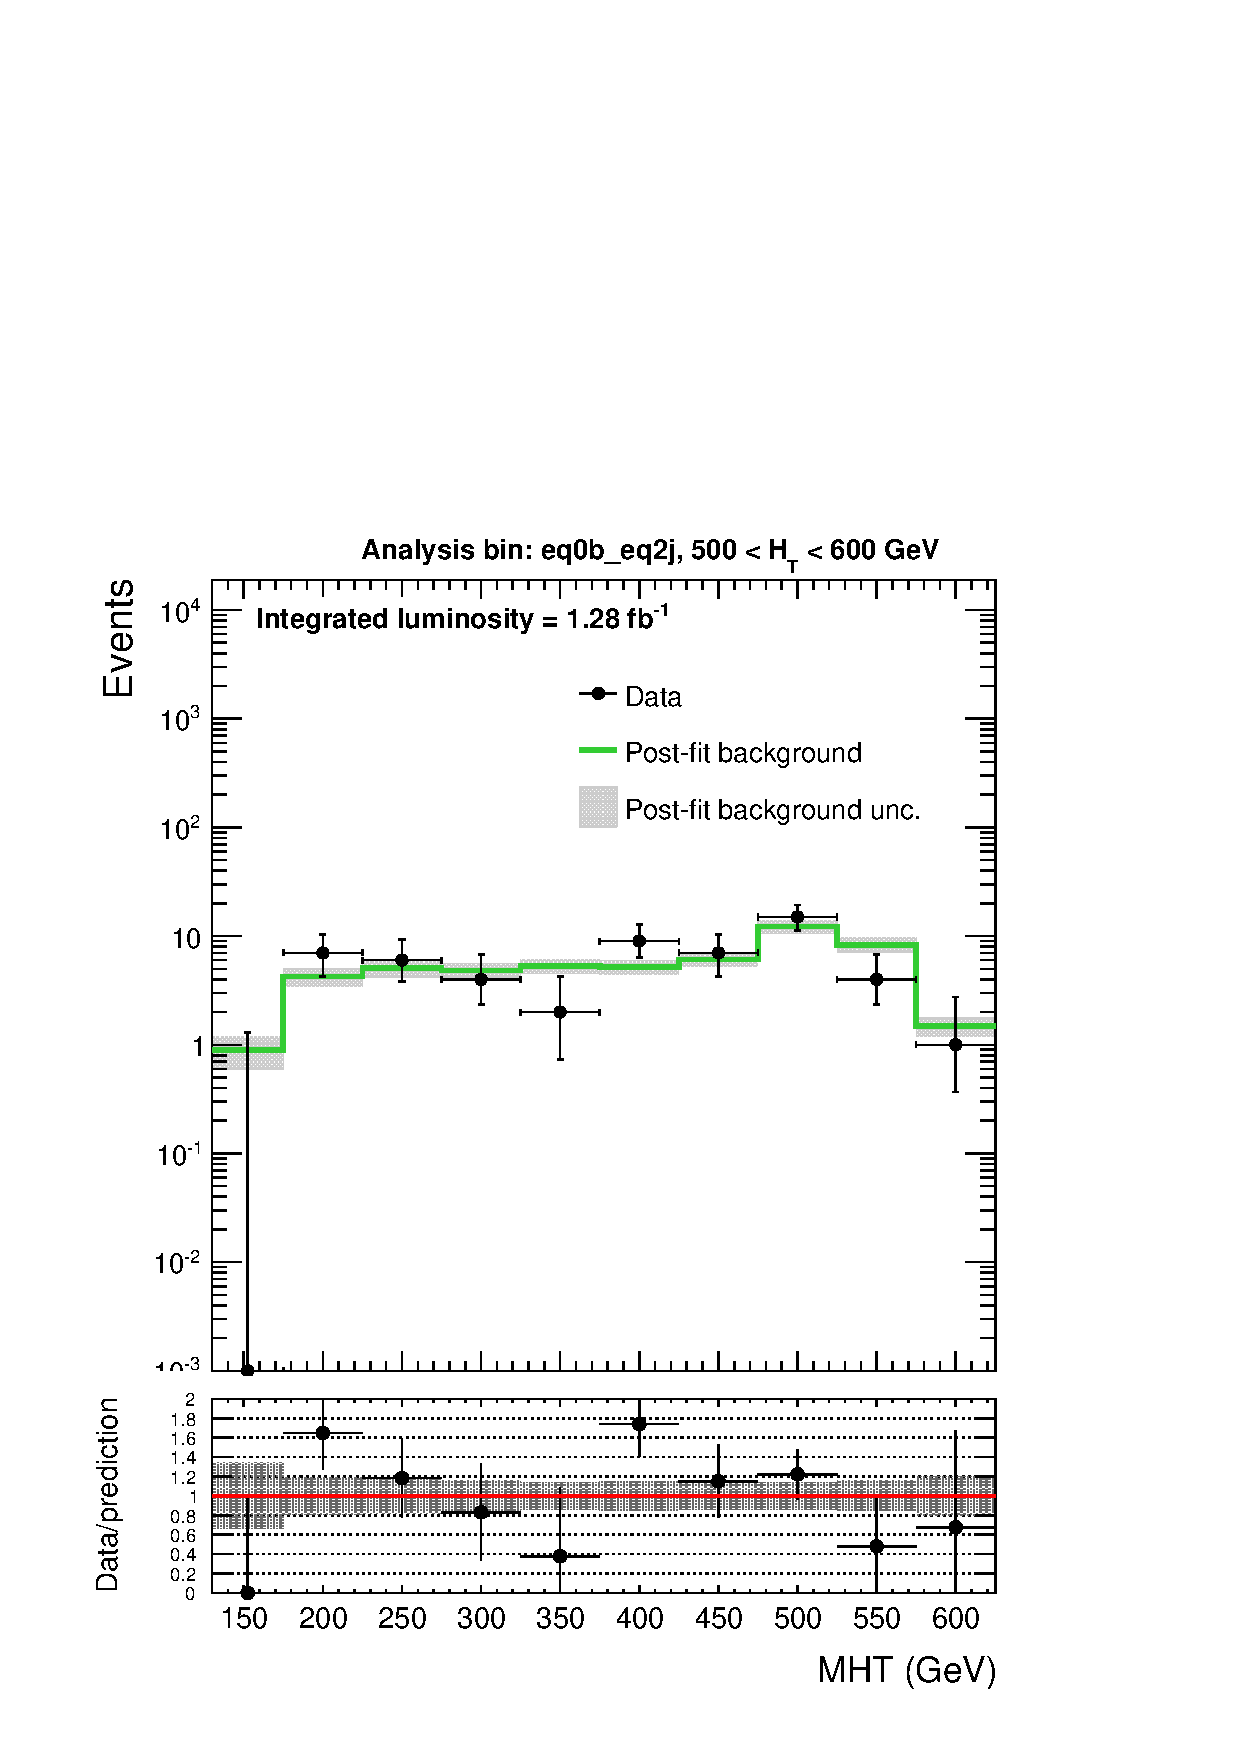
\includegraphics[width=0.25\textwidth]{figures/postFitResults/postFitShape_eq0b_eq2j_500_600.pdf} }\\
    \subfigure[$\nj^{\mathrm{sym}}=2$, $\nb=0$, $600 < \scalht < 800 \; \mathrm{GeV}$]{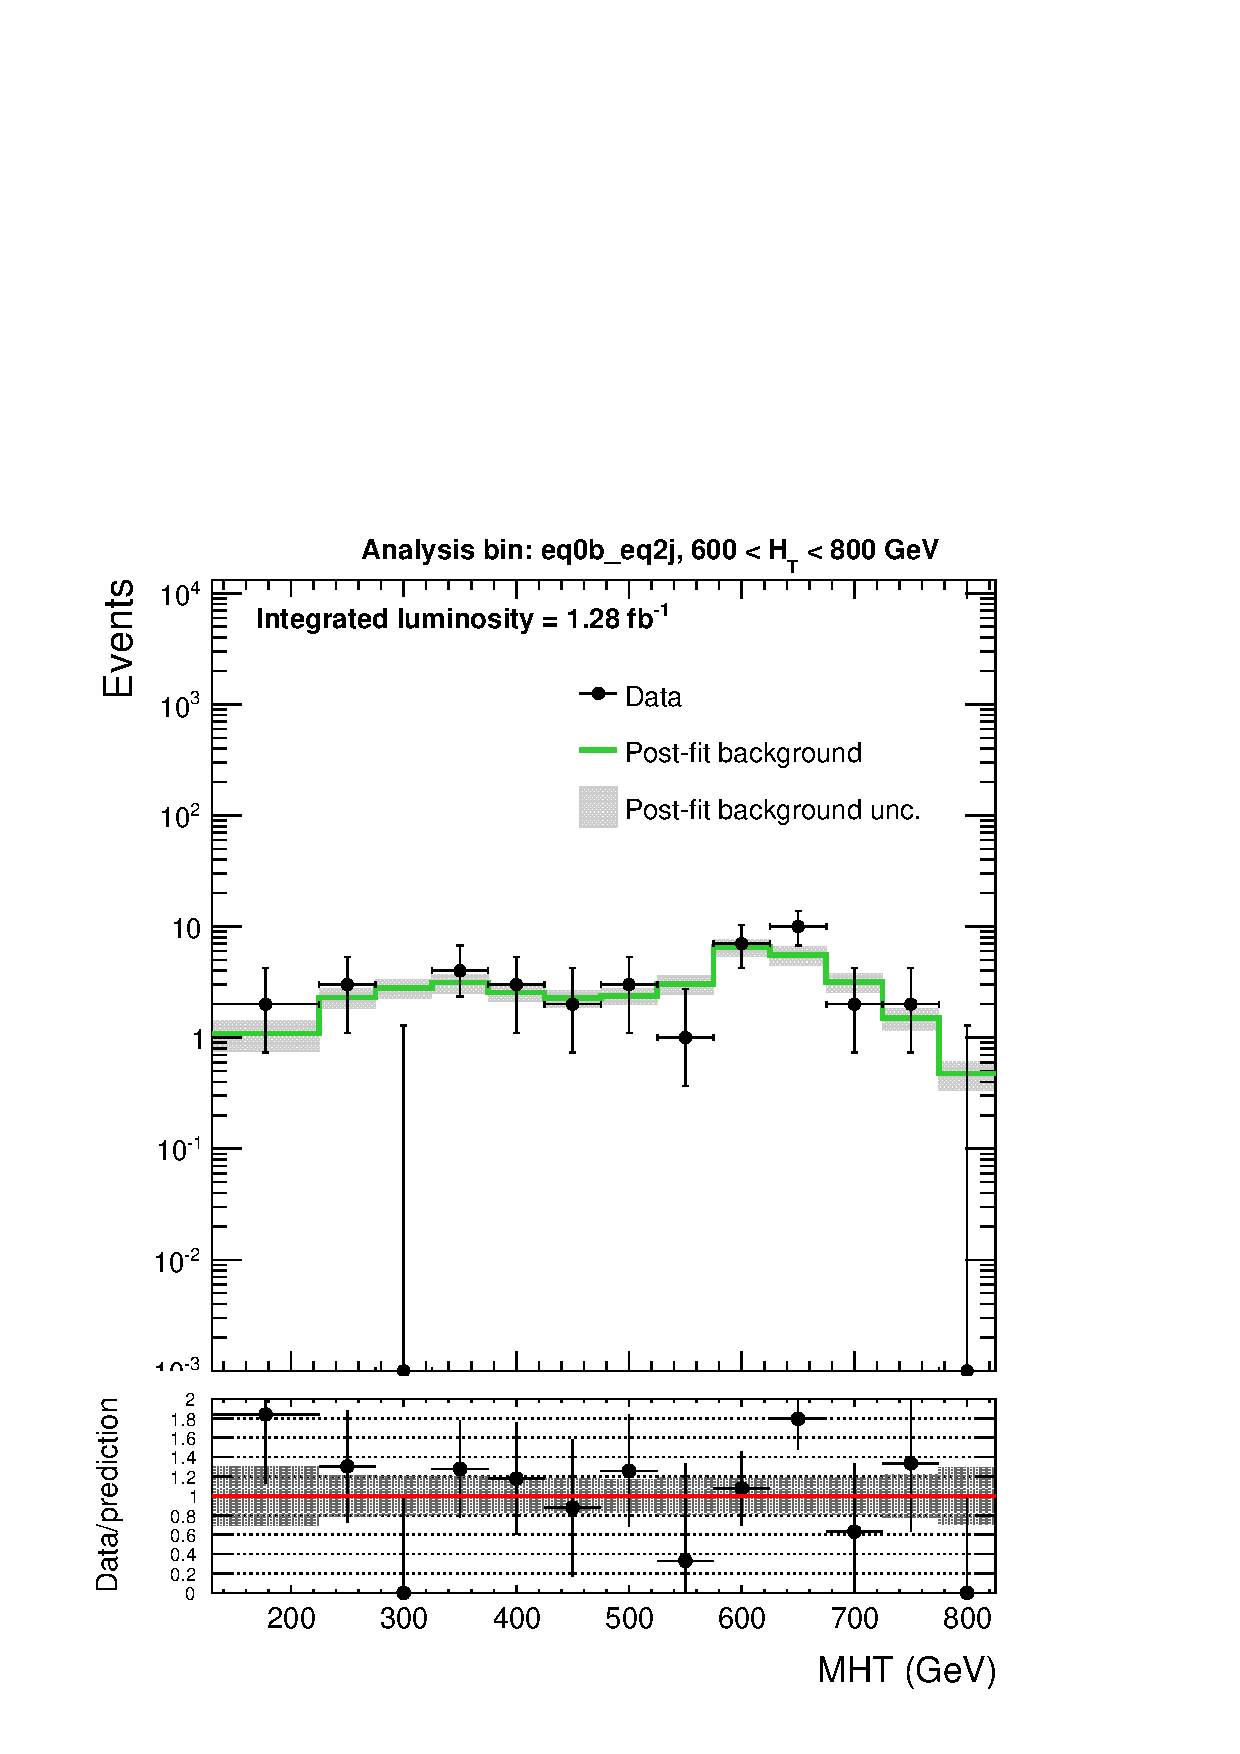
\includegraphics[width=0.25\textwidth]{figures/postFitResults/postFitShape_eq0b_eq2j_600_800.pdf} }\hspace{1cm}
    \subfigure[$\nj^{\mathrm{sym}}=2$, $\nb=0$, $\scalht > 800 \; \mathrm{GeV}$]{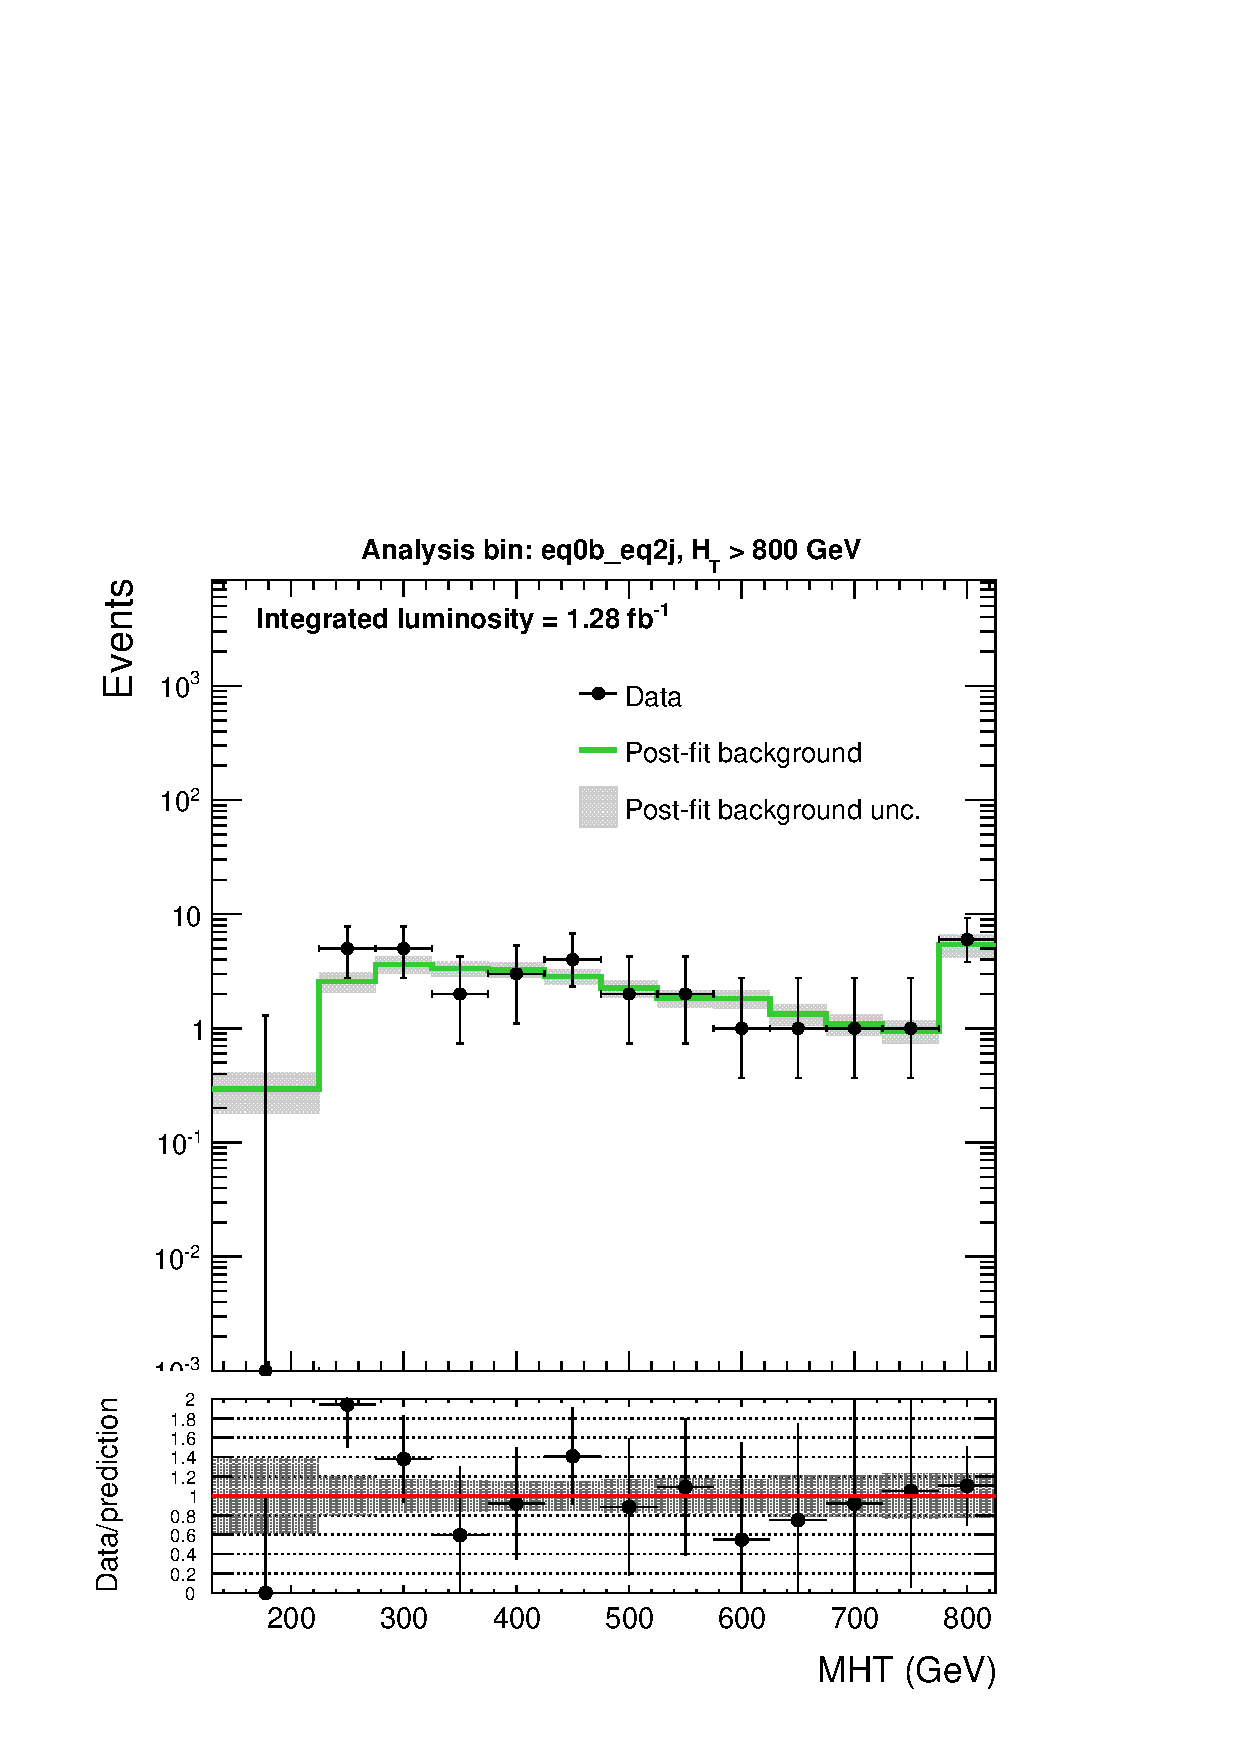
\includegraphics[width=0.25\textwidth]{figures/postFitResults/postFitShape_eq0b_eq2j_800_Inf.pdf} }\hspace{1cm}
  \end{center}
\end{figure}



\newpage
\begin{figure}[h!]
\caption{Post-fit \MHT templates for the bin $\nj^{\mathrm{asym}}=3$, $\nb=0$ \label{fig:postFitShapes_eq0b_eq3a}}.
\begin{center}

    \subfigure[$\nj^{\mathrm{asym}}=3$, $\nb=0$, $200 < \scalht < 250 \; \mathrm{GeV}$]{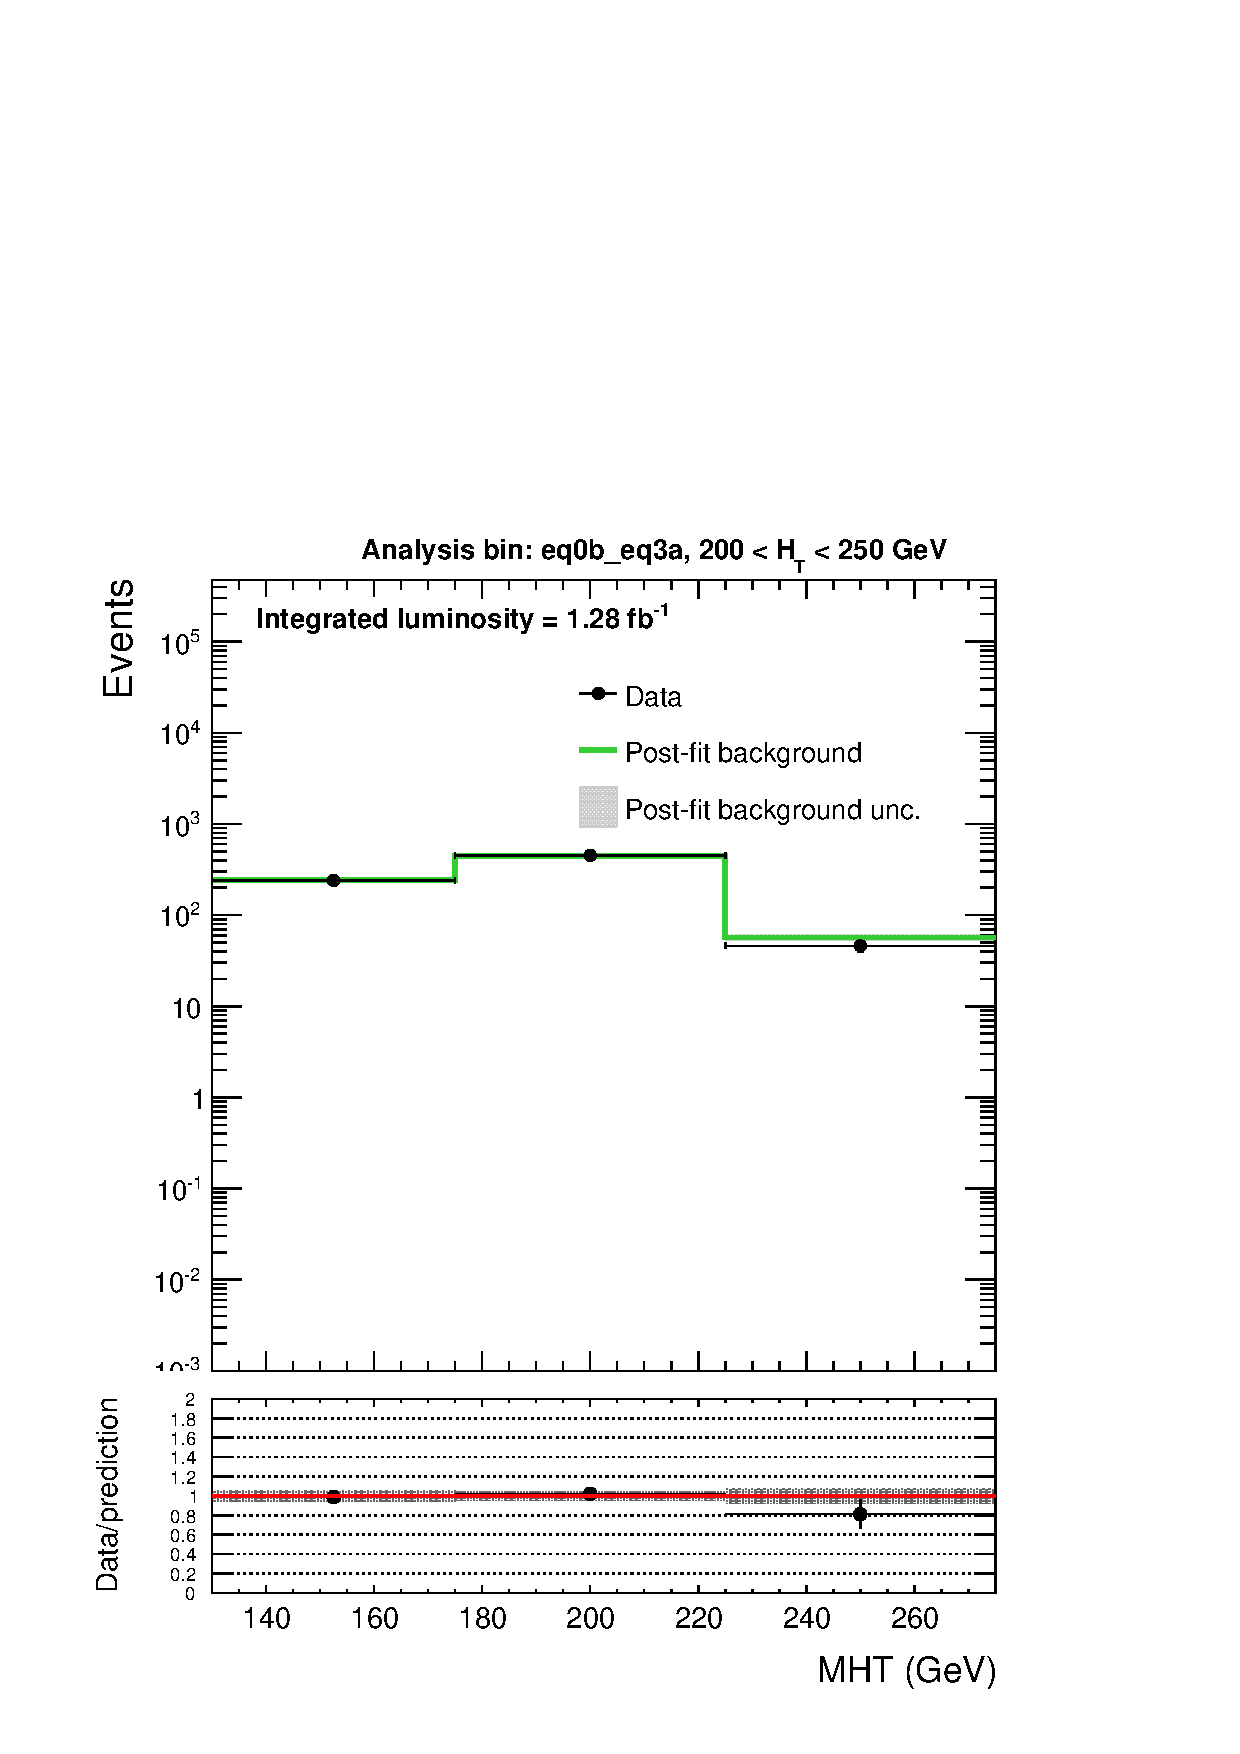
\includegraphics[width=0.25\textwidth]{figures/postFitResults/postFitShape_eq0b_eq3a_200_250.pdf} }\hspace{1cm}
    \subfigure[$\nj^{\mathrm{asym}}=3$, $\nb=0$, $250 < \scalht < 300 \; \mathrm{GeV}$]{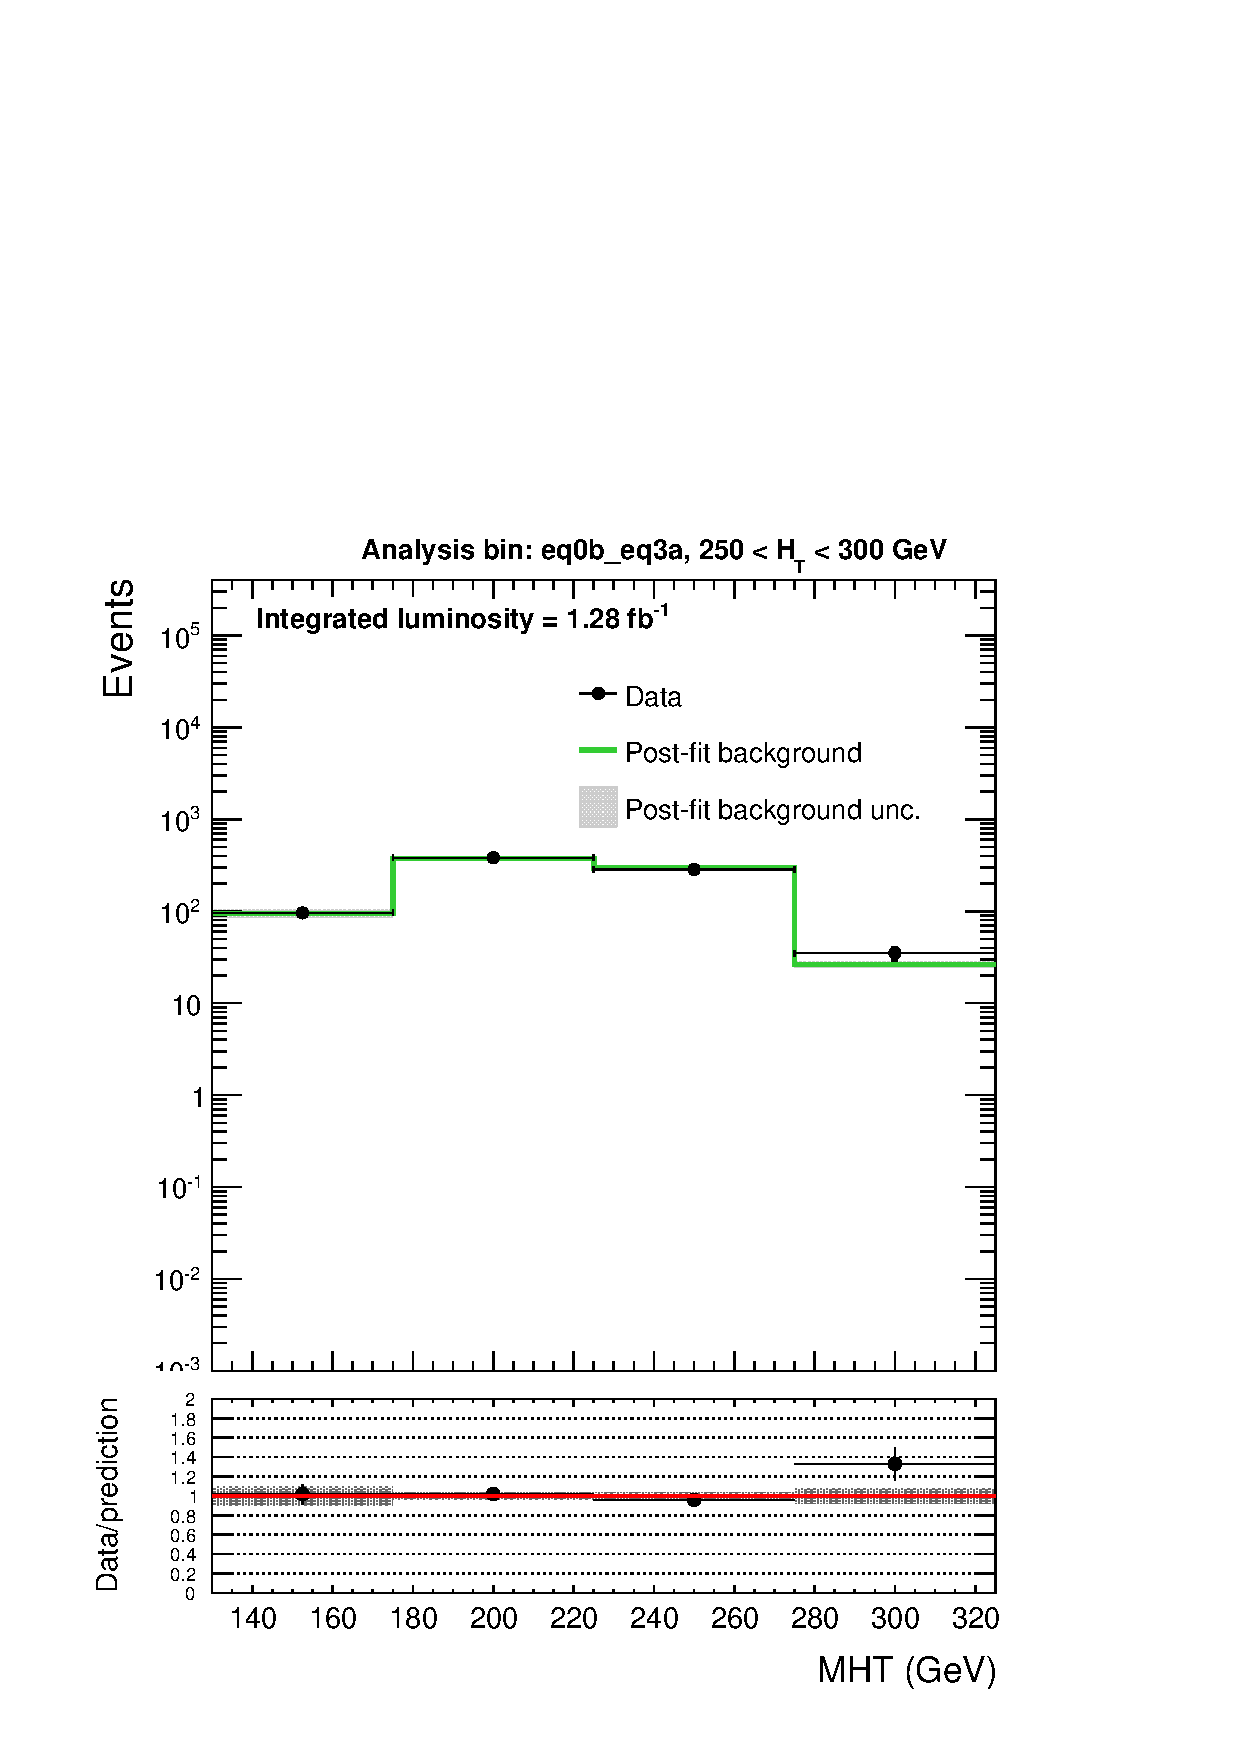
\includegraphics[width=0.25\textwidth]{figures/postFitResults/postFitShape_eq0b_eq3a_250_300.pdf} }\hspace{1cm}
    \subfigure[$\nj^{\mathrm{asym}}=3$, $\nb=0$, $300 < \scalht < 350 \; \mathrm{GeV}$]{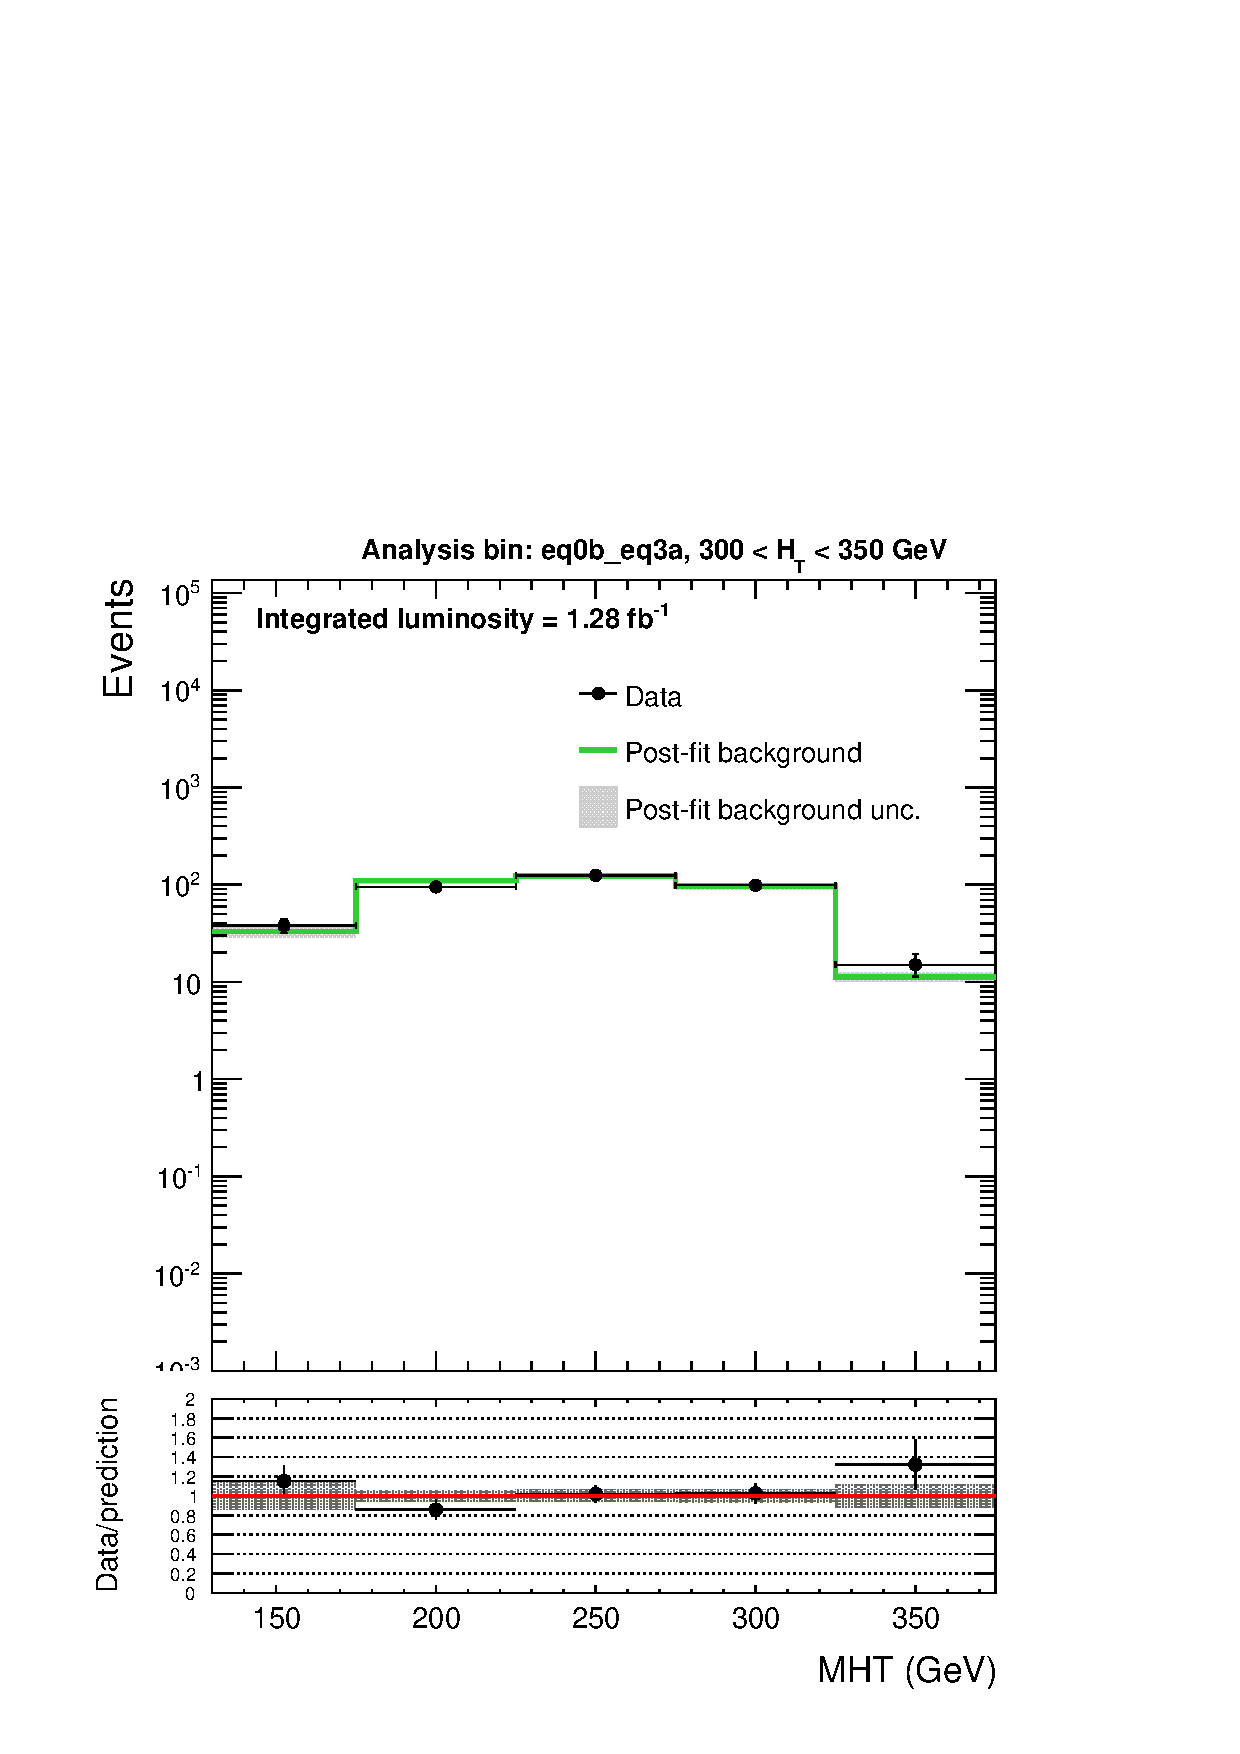
\includegraphics[width=0.25\textwidth]{figures/postFitResults/postFitShape_eq0b_eq3a_300_350.pdf} }\\
    \subfigure[$\nj^{\mathrm{asym}}=3$, $\nb=0$, $350 < \scalht < 400 \; \mathrm{GeV}$]{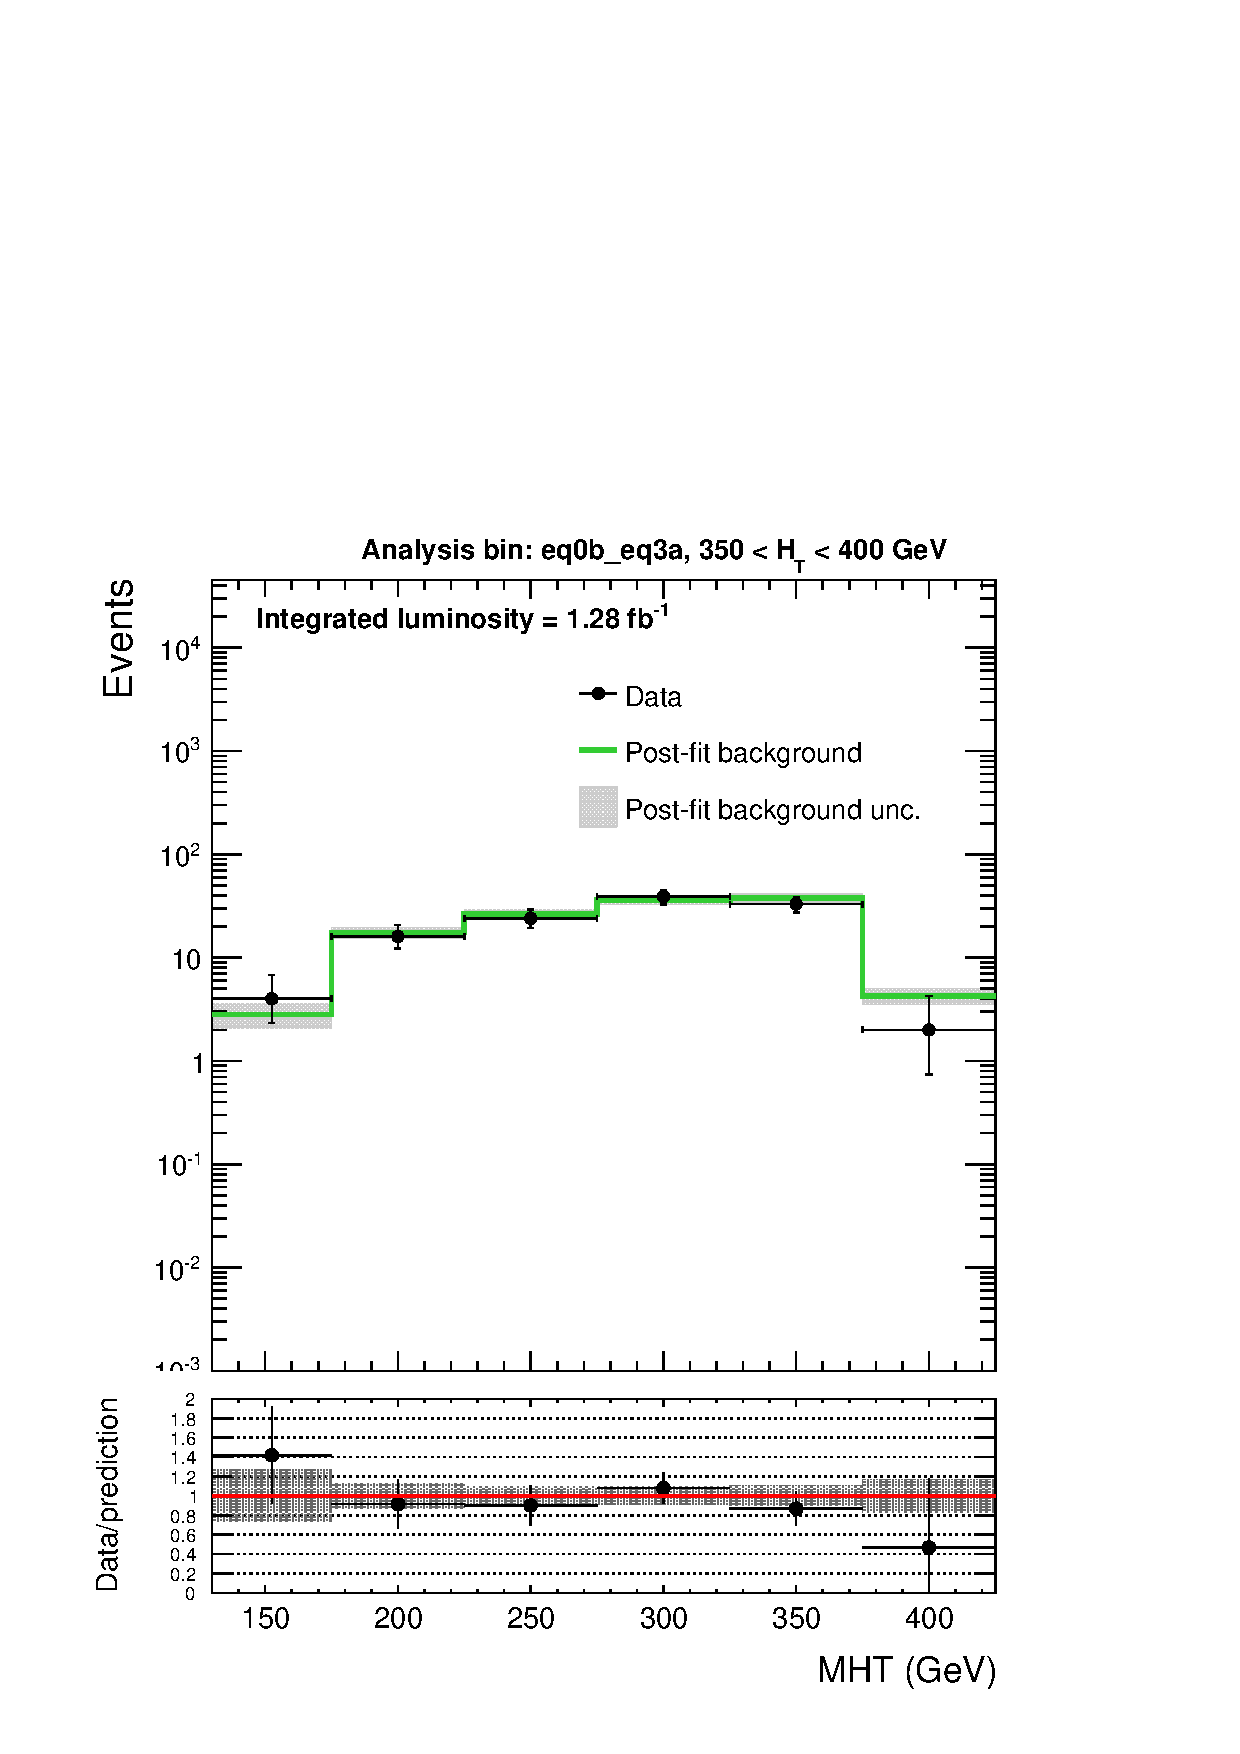
\includegraphics[width=0.25\textwidth]{figures/postFitResults/postFitShape_eq0b_eq3a_350_400.pdf} }\hspace{1cm}
    \subfigure[$\nj^{\mathrm{asym}}=3$, $\nb=0$, $400 < \scalht < 500 \; \mathrm{GeV}$]{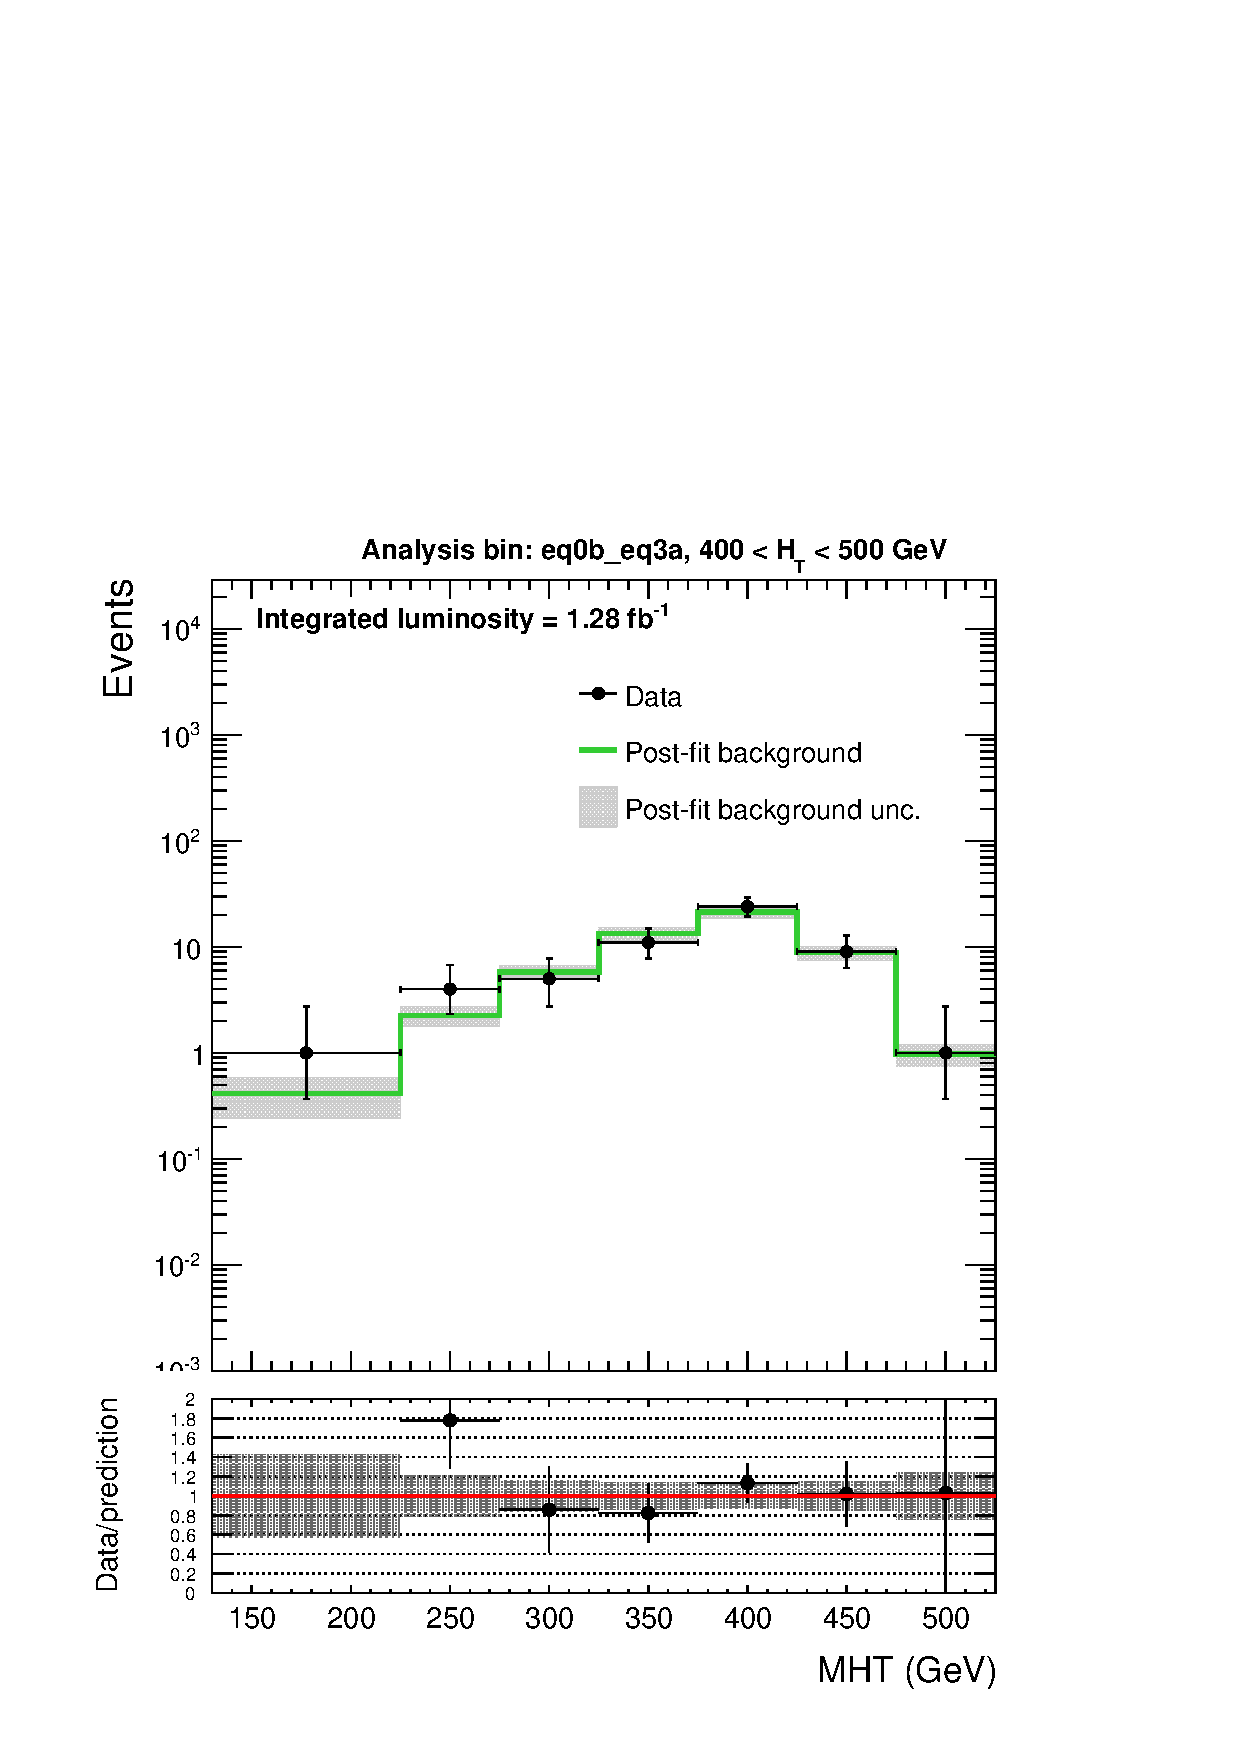
\includegraphics[width=0.25\textwidth]{figures/postFitResults/postFitShape_eq0b_eq3a_400_500.pdf} }\hspace{1cm}
    \subfigure[$\nj^{\mathrm{asym}}=3$, $\nb=0$, $500 < \scalht < 600 \; \mathrm{GeV}$]{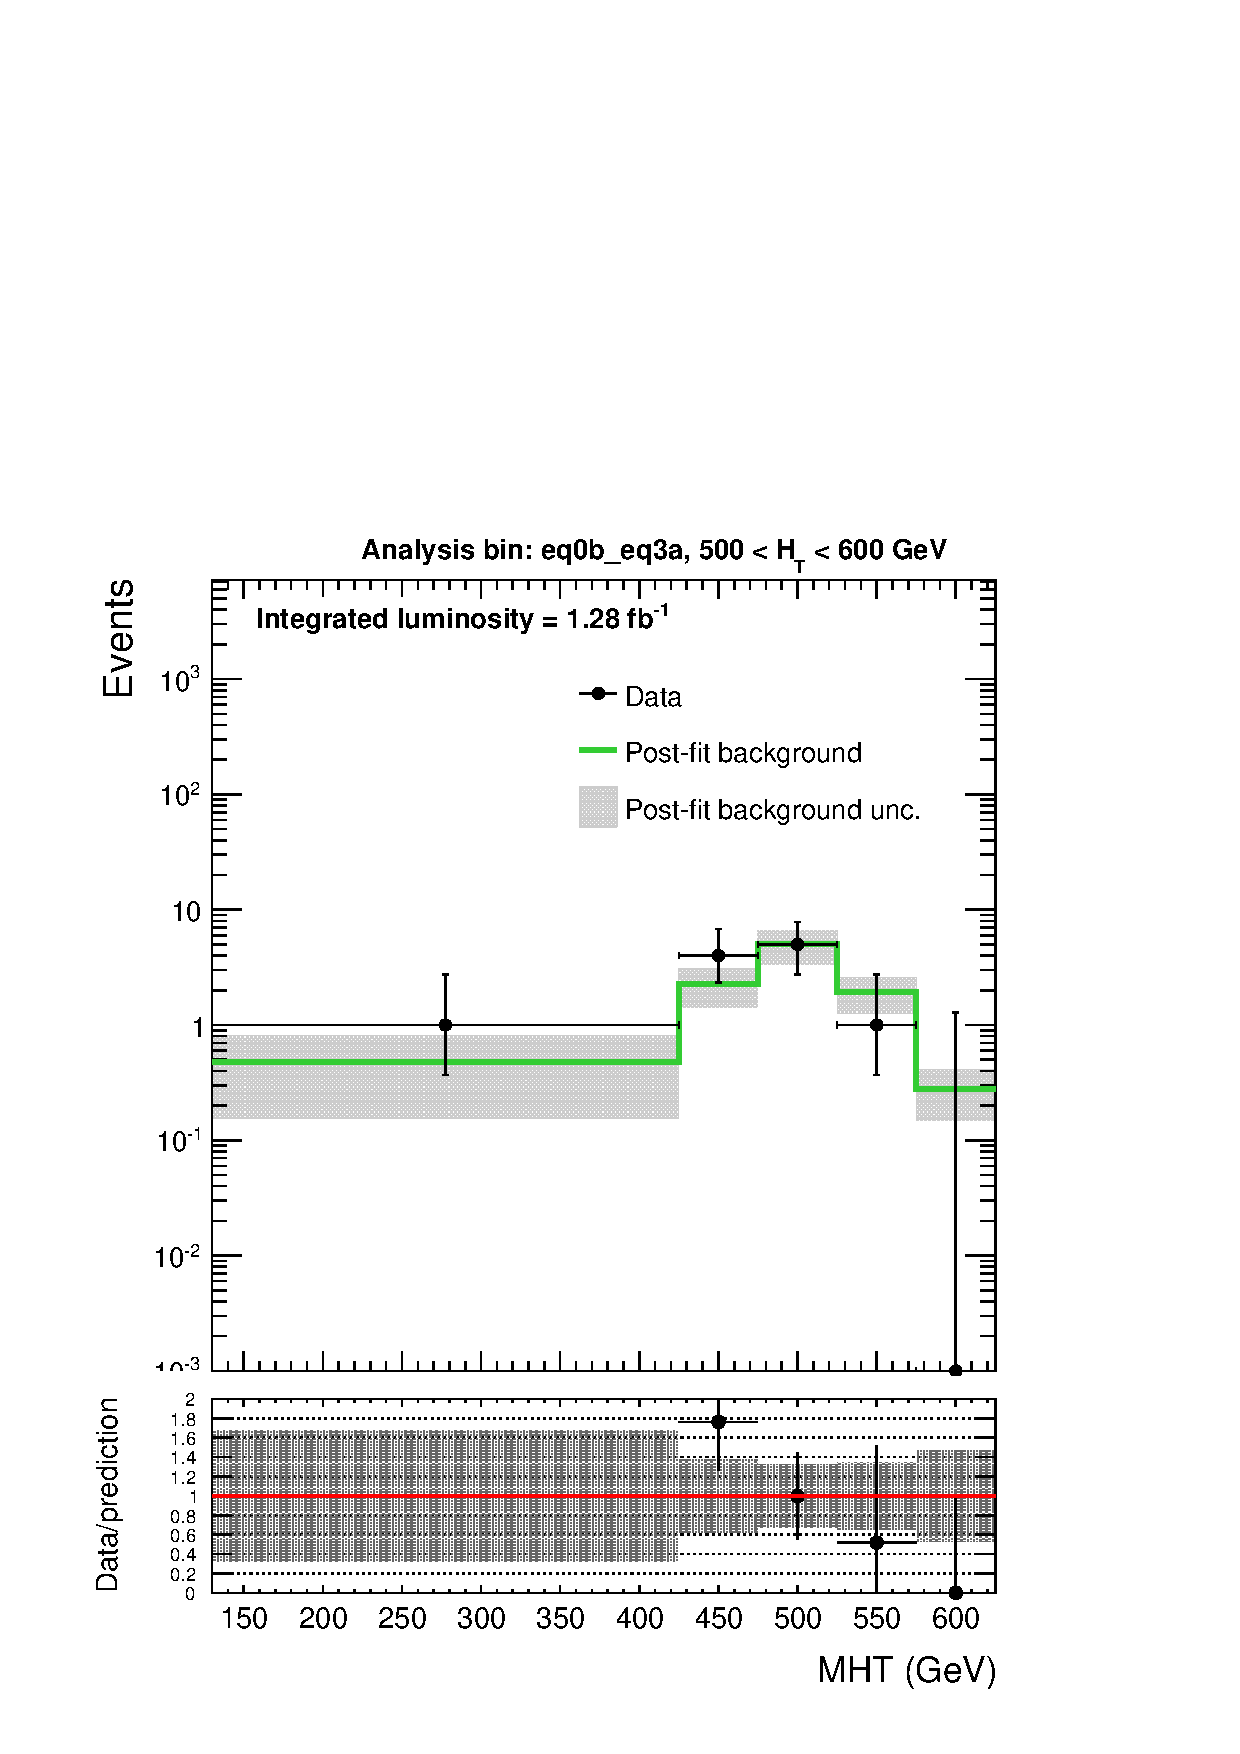
\includegraphics[width=0.25\textwidth]{figures/postFitResults/postFitShape_eq0b_eq3a_500_600.pdf} }\\
    \subfigure[$\nj^{\mathrm{asym}}=3$, $\nb=0$, $\scalht > 600 \; \mathrm{GeV}$]{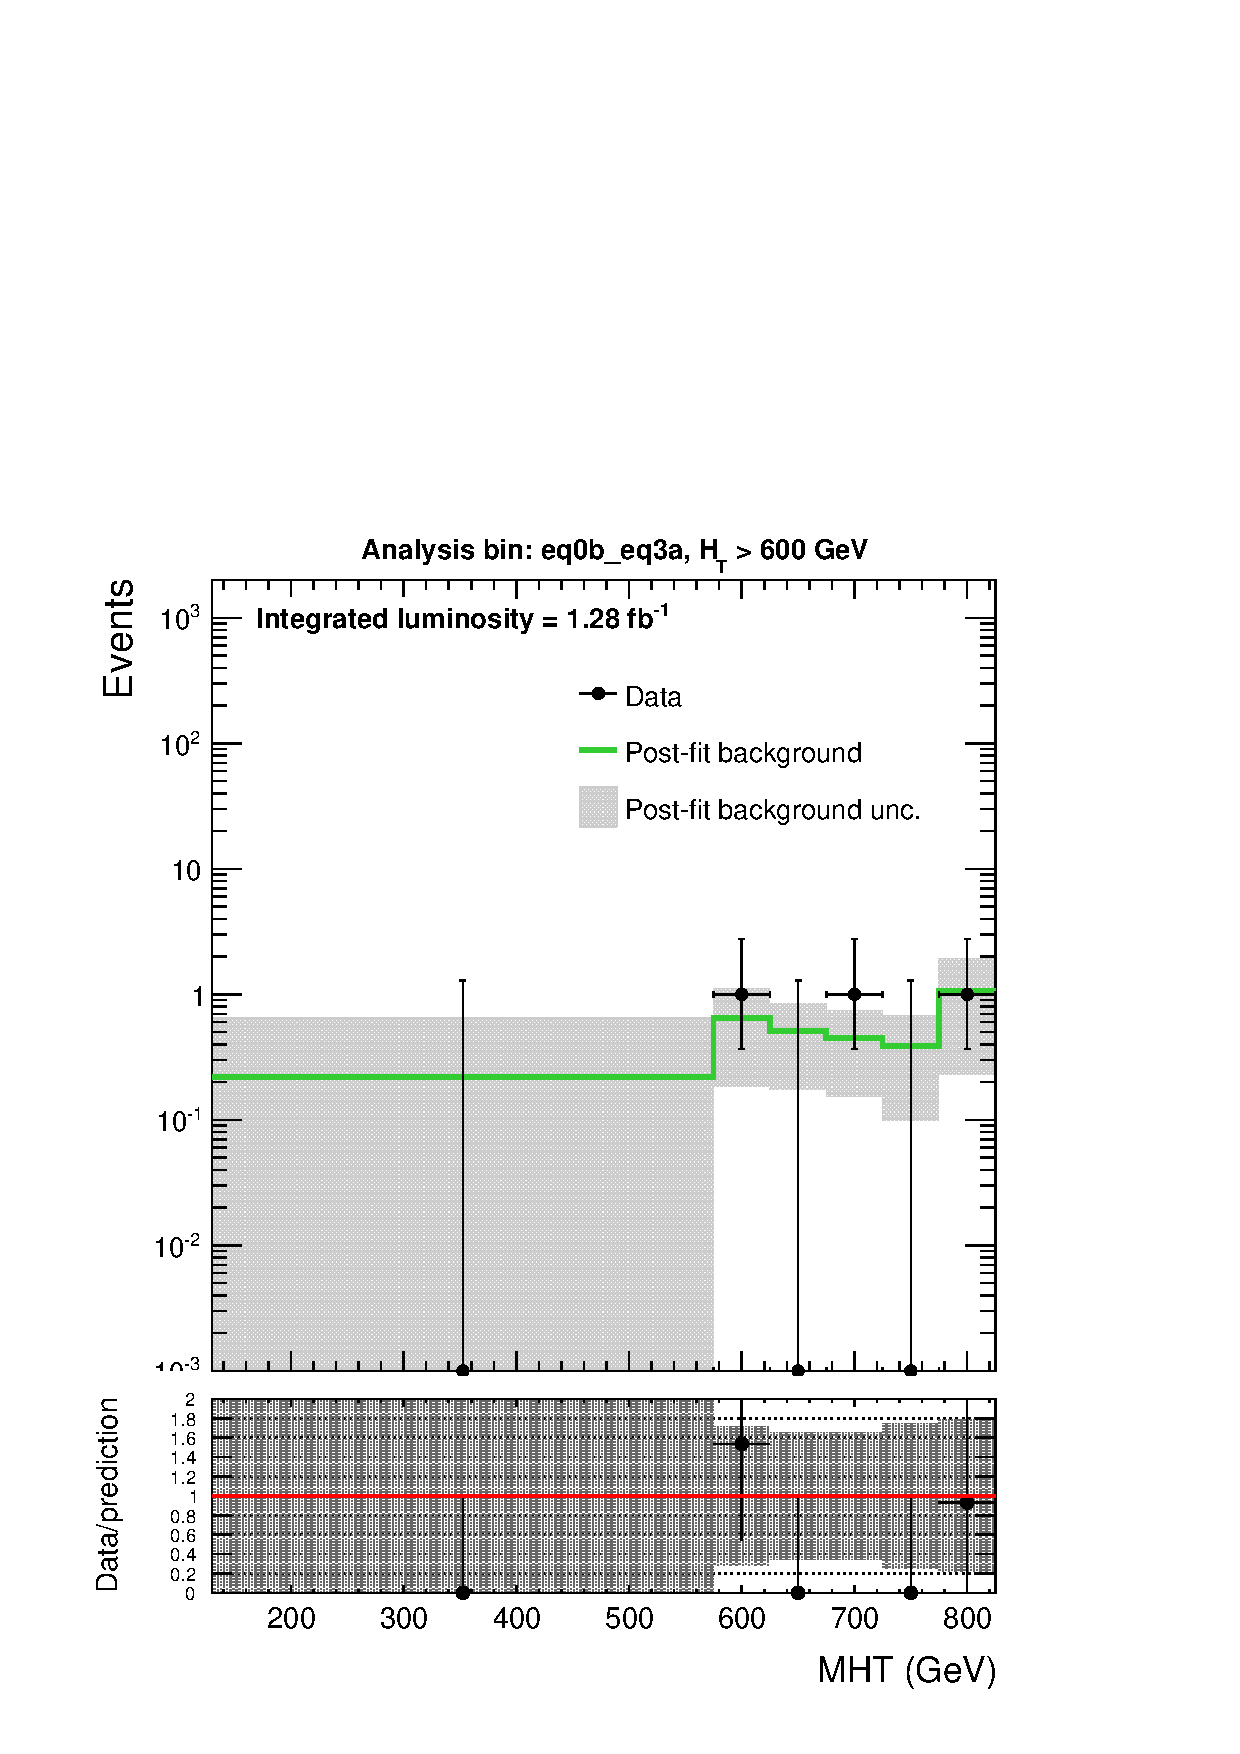
\includegraphics[width=0.25\textwidth]{figures/postFitResults/postFitShape_eq0b_eq3a_600_Inf.pdf} }\hspace{1cm}
  \end{center}
\end{figure}



\newpage
\begin{figure}[h!]
\caption{Post-fit \MHT templates for the bin $\nj^{\mathrm{sym}}=3$, $\nb=0$ \label{fig:postFitShapes_eq0b_eq3j}}.
\begin{center}

    \subfigure[$\nj^{\mathrm{sym}}=3$, $\nb=0$, $250 < \scalht < 300 \; \mathrm{GeV}$]{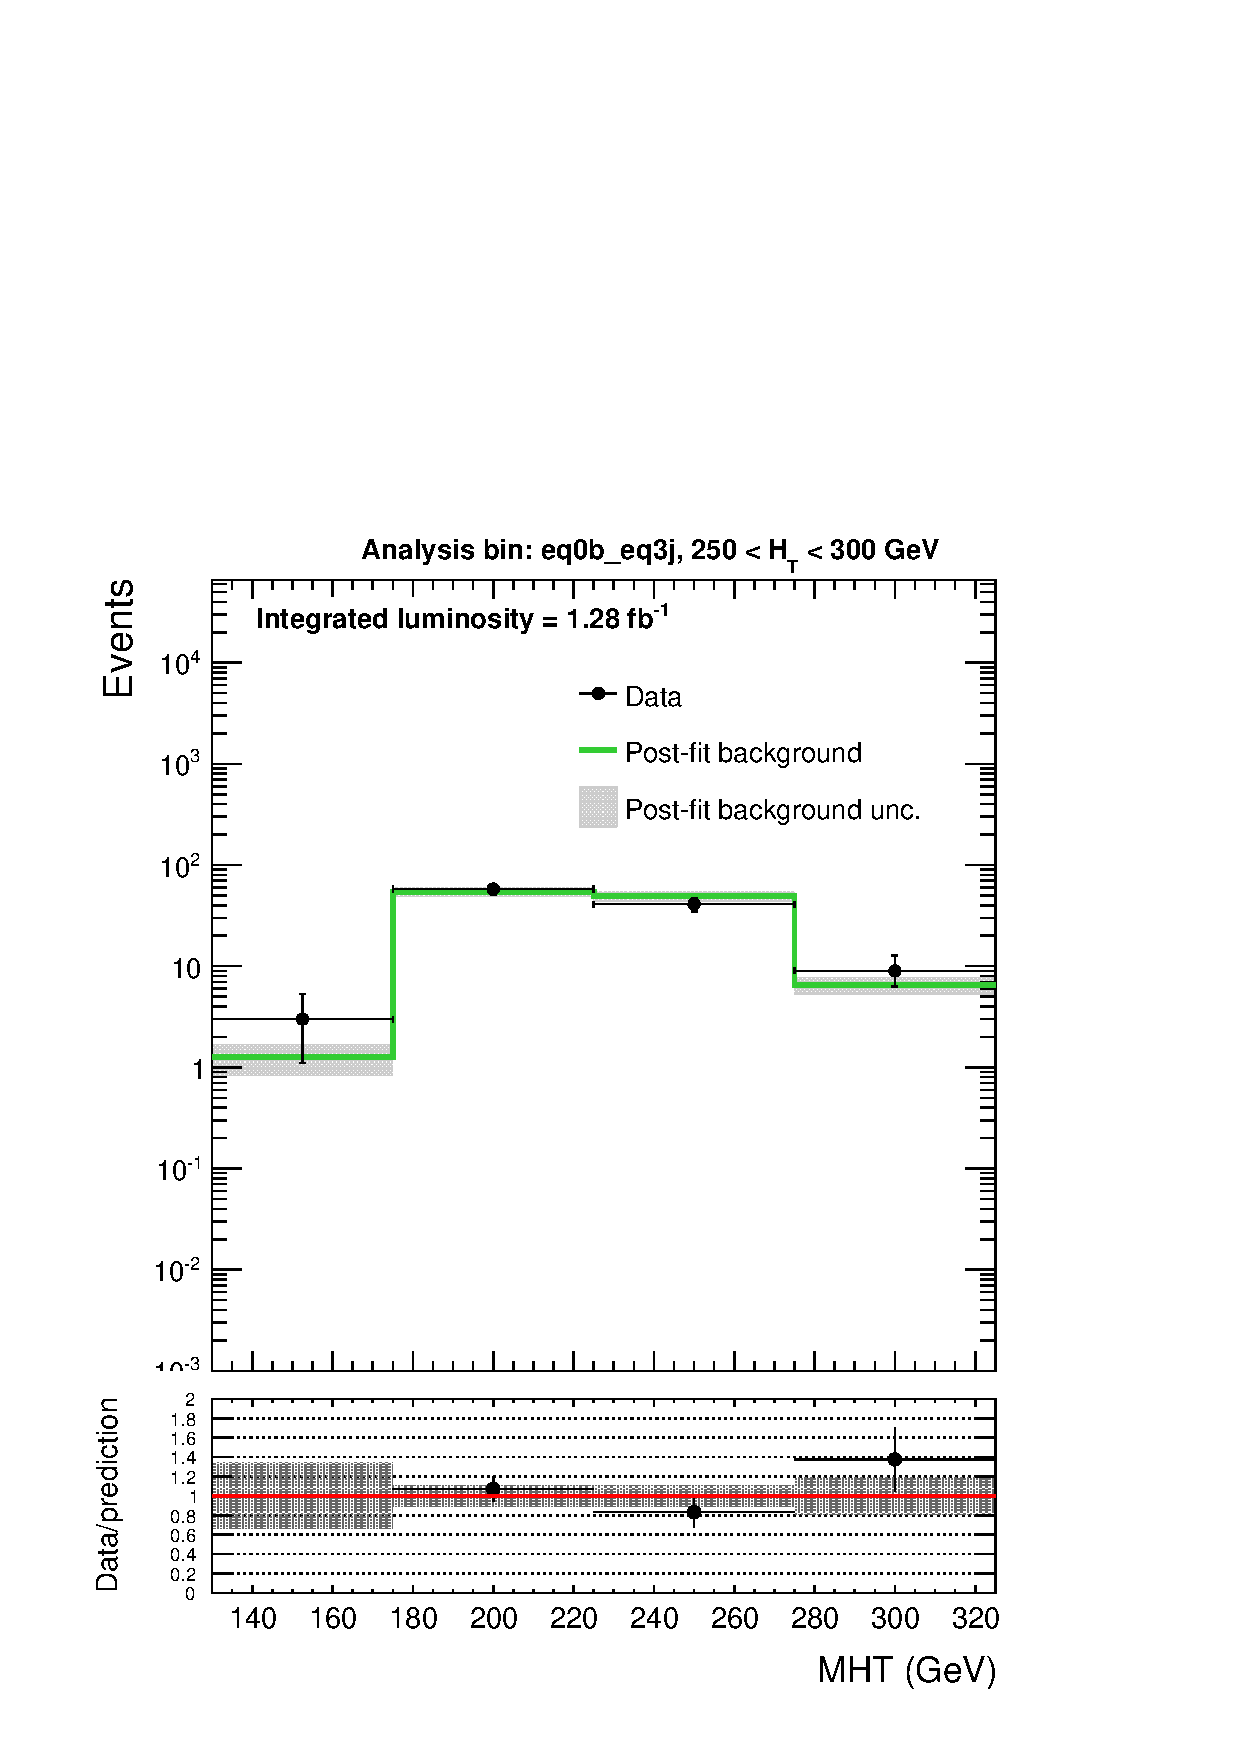
\includegraphics[width=0.25\textwidth]{figures/postFitResults/postFitShape_eq0b_eq3j_250_300.pdf} }\hspace{1cm}
    \subfigure[$\nj^{\mathrm{sym}}=3$, $\nb=0$, $300 < \scalht < 350 \; \mathrm{GeV}$]{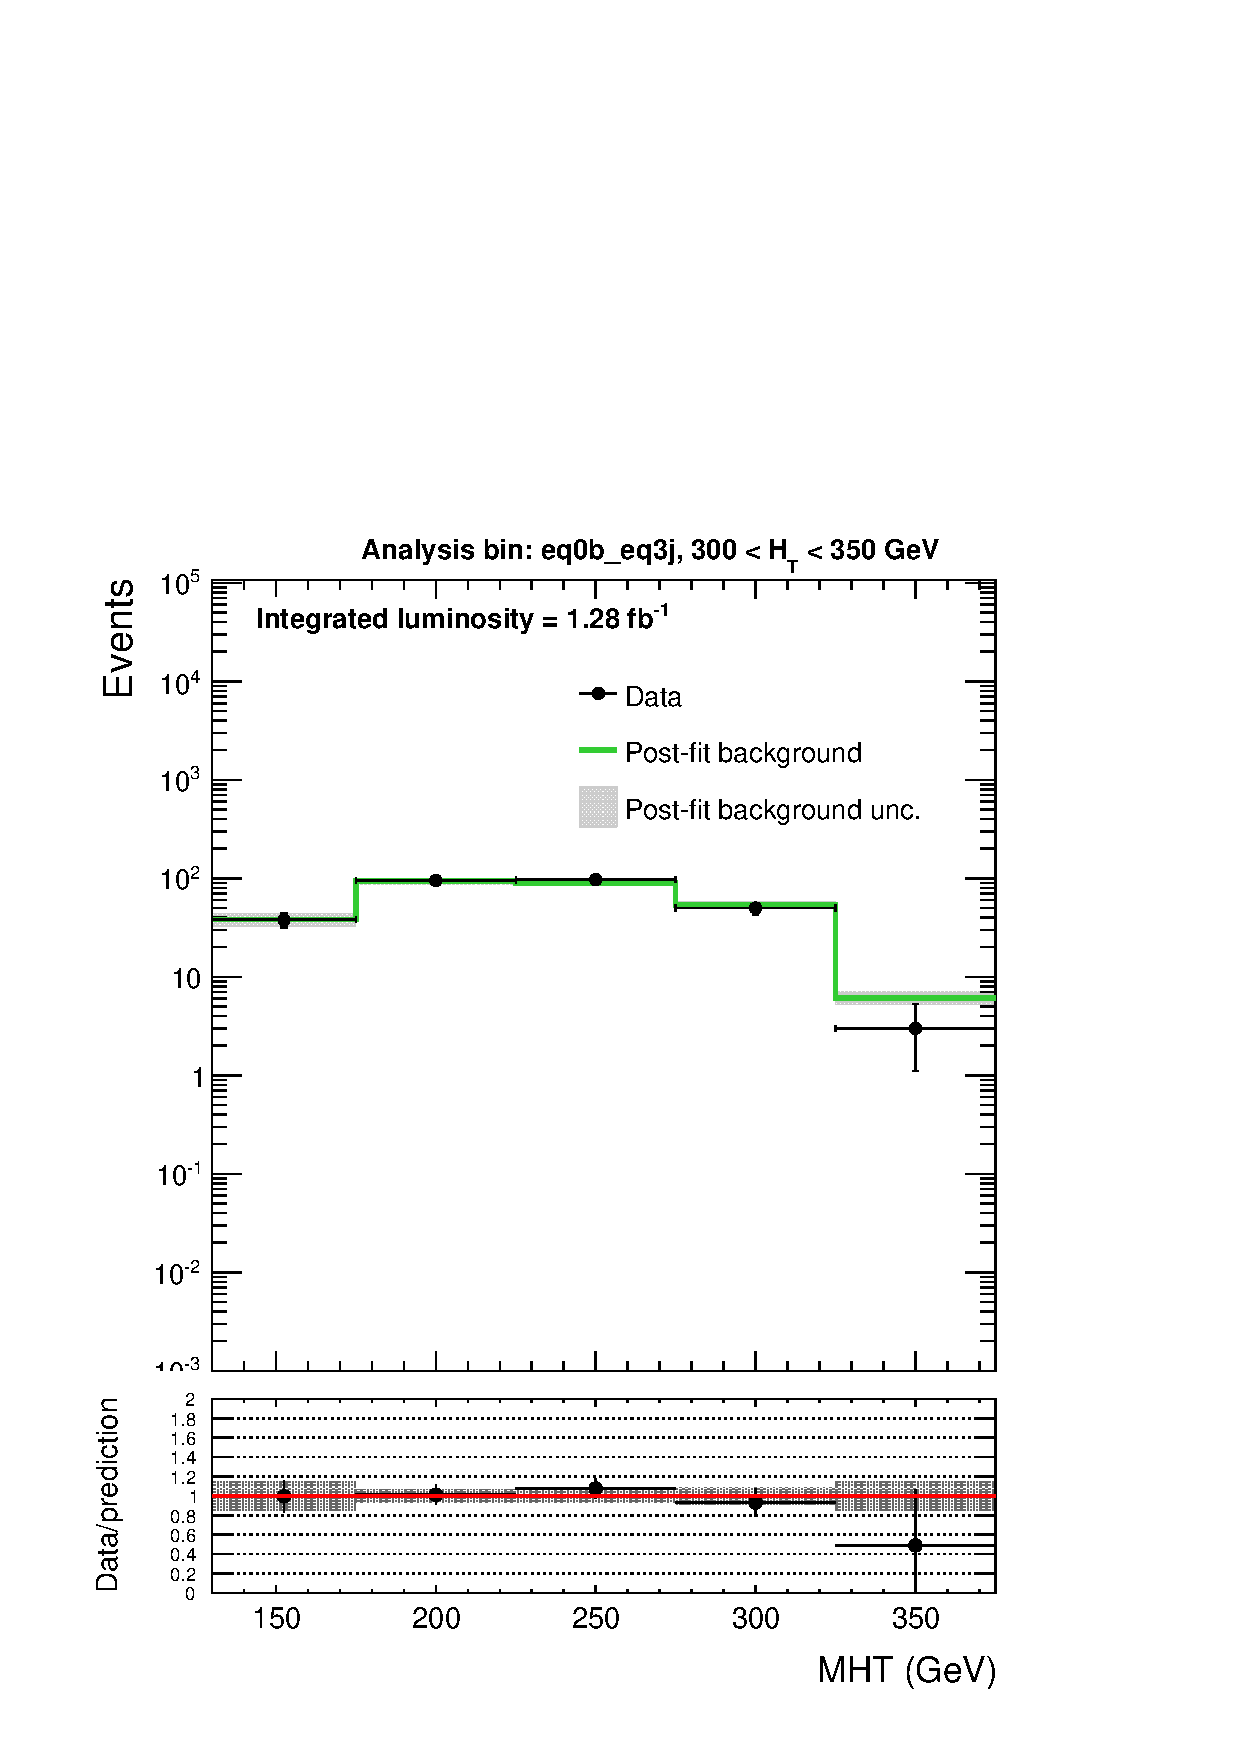
\includegraphics[width=0.25\textwidth]{figures/postFitResults/postFitShape_eq0b_eq3j_300_350.pdf} }\hspace{1cm}
    \subfigure[$\nj^{\mathrm{sym}}=3$, $\nb=0$, $350 < \scalht < 400 \; \mathrm{GeV}$]{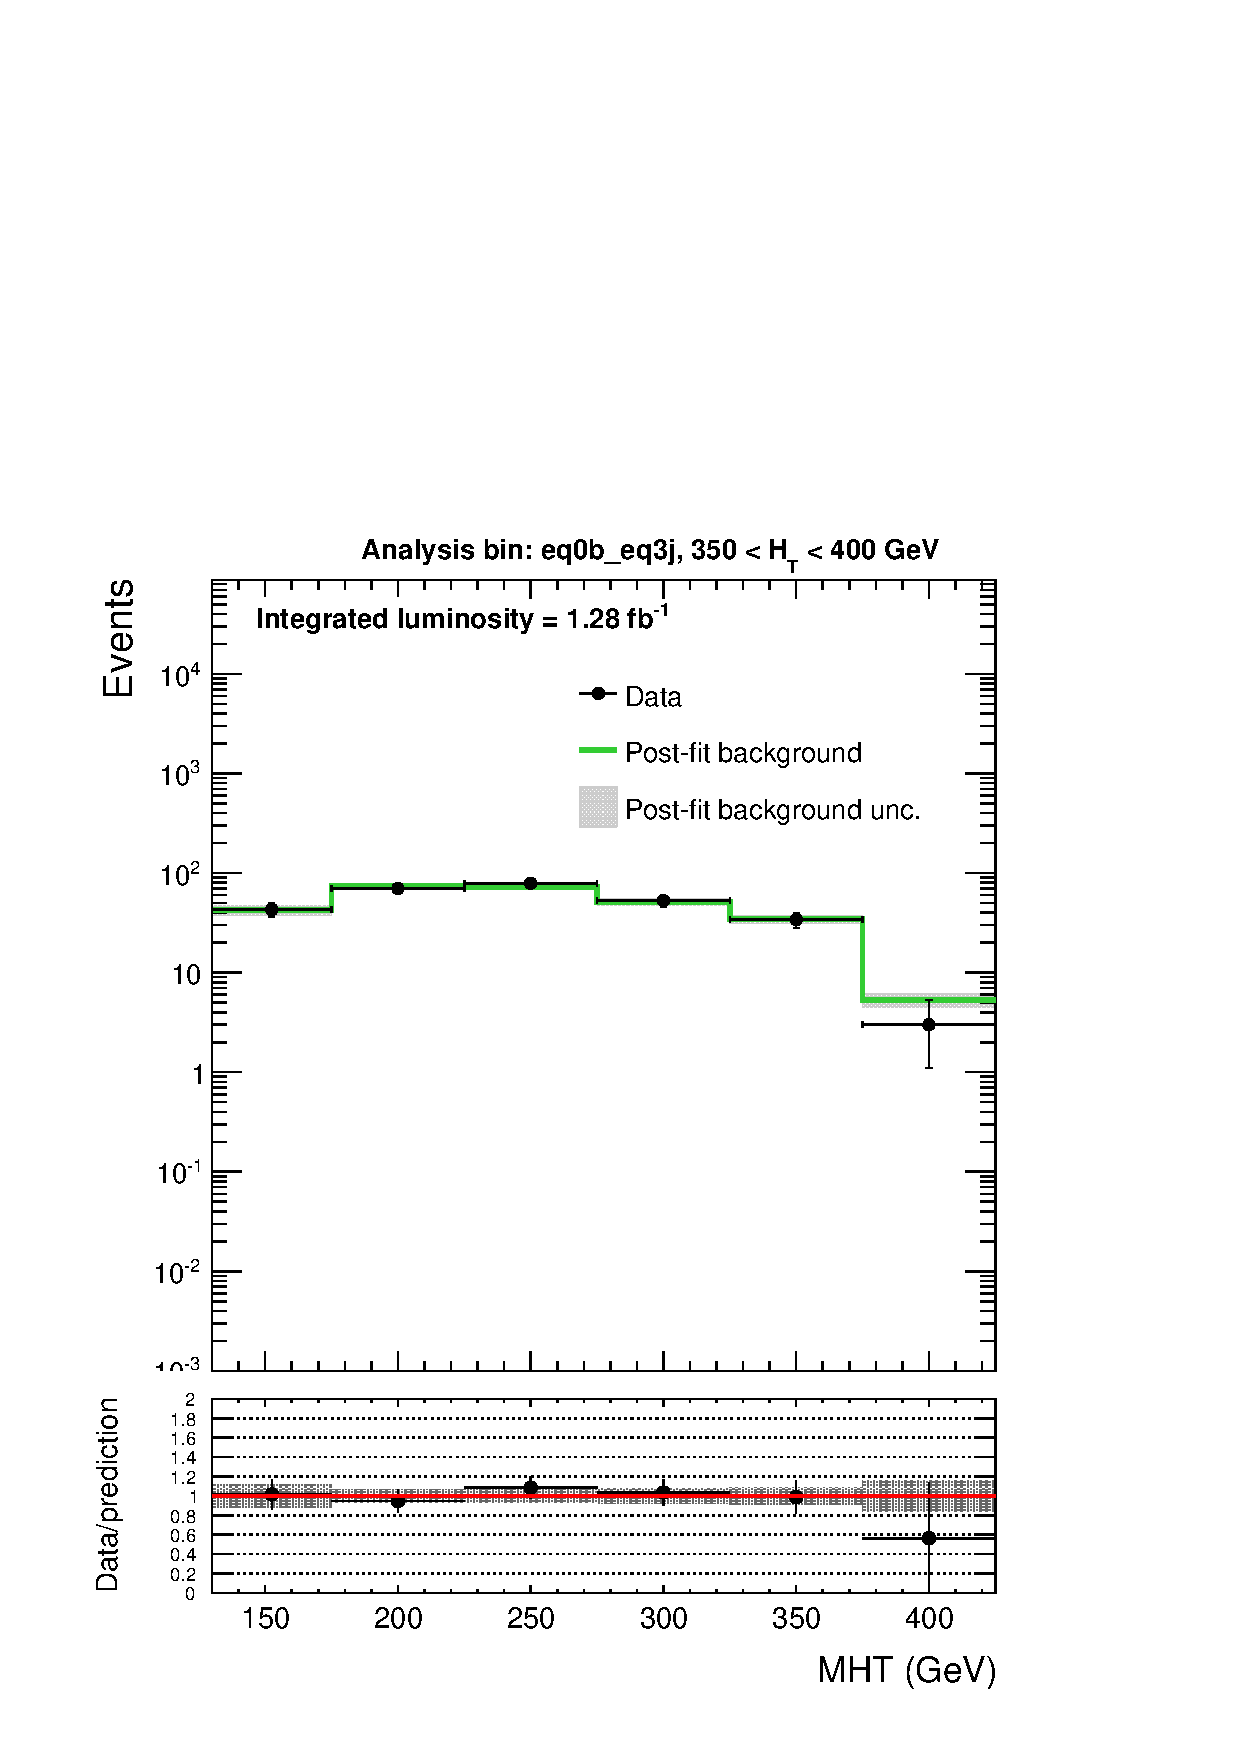
\includegraphics[width=0.25\textwidth]{figures/postFitResults/postFitShape_eq0b_eq3j_350_400.pdf} }\\
    \subfigure[$\nj^{\mathrm{sym}}=3$, $\nb=0$, $400 < \scalht < 500 \; \mathrm{GeV}$]{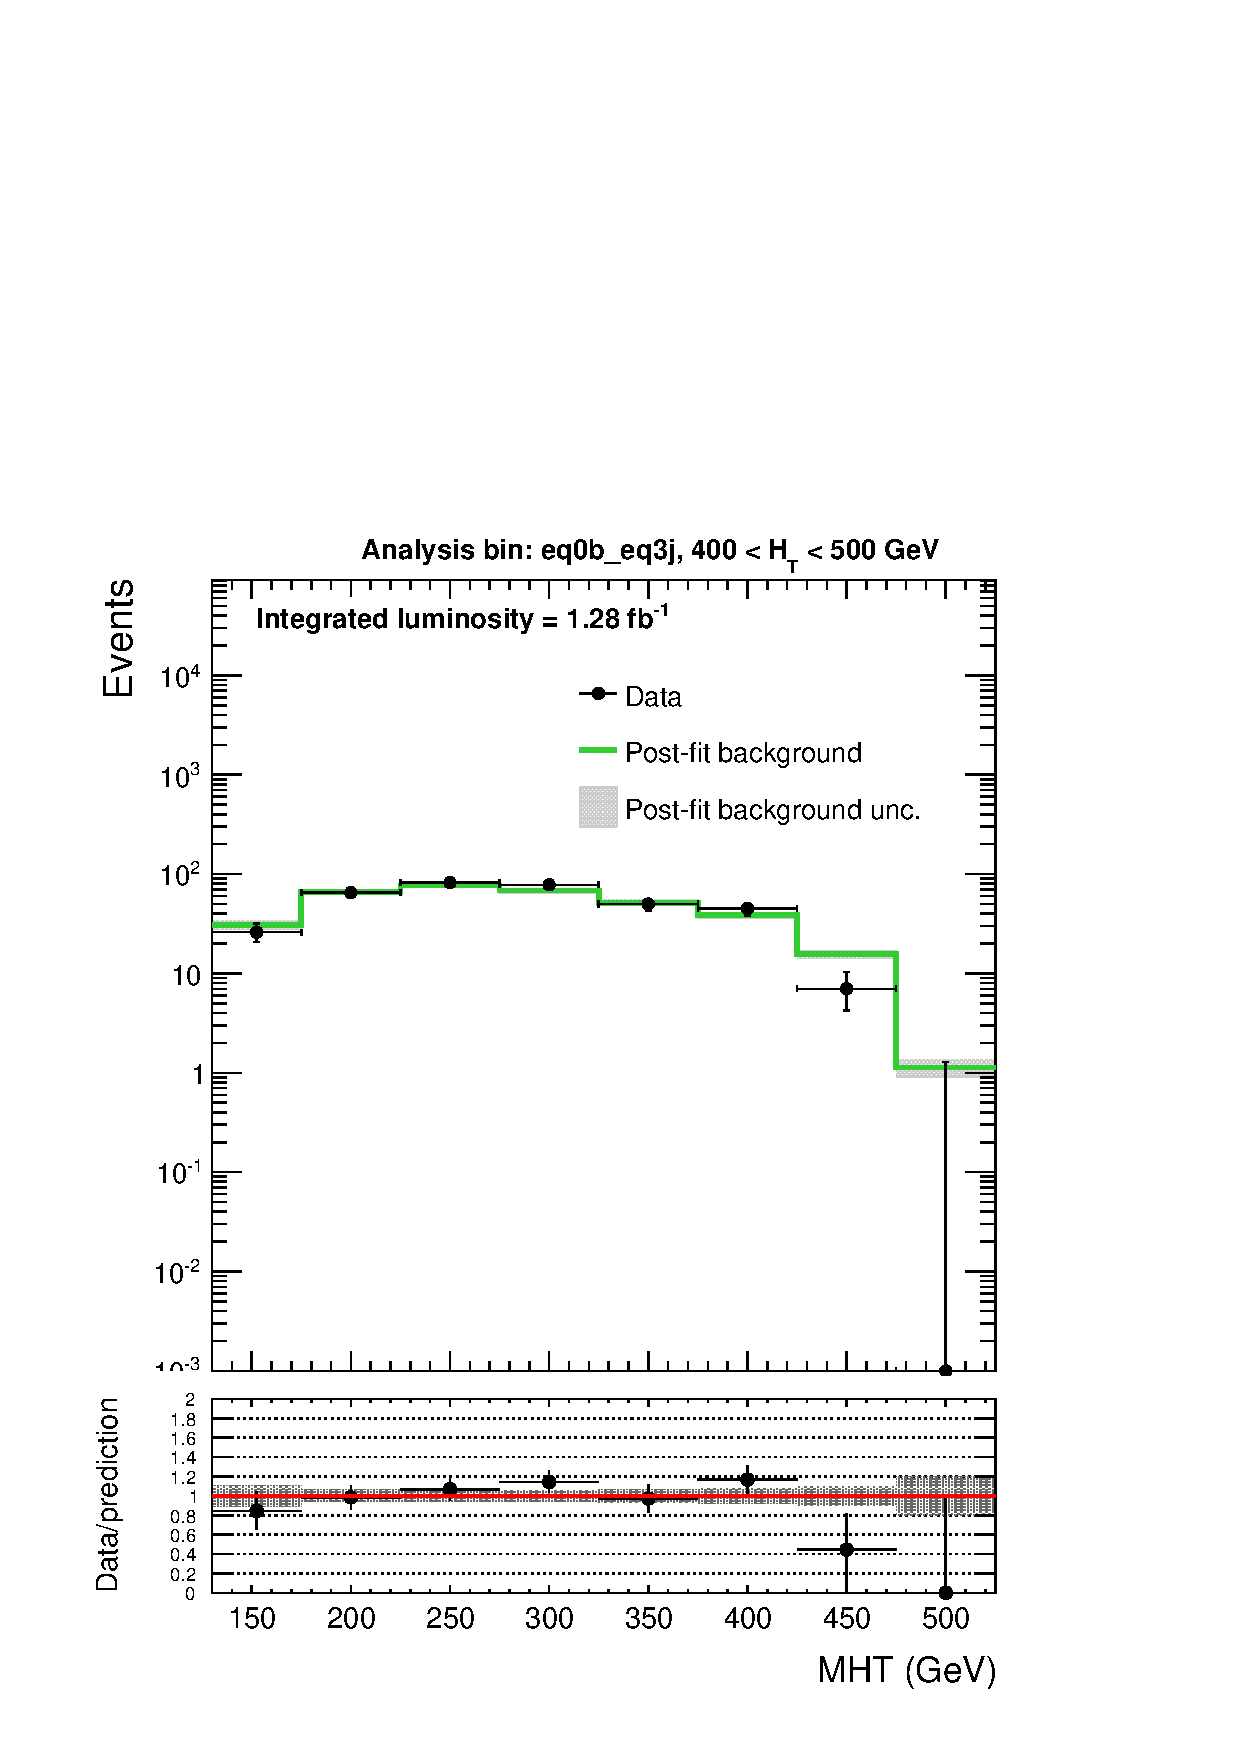
\includegraphics[width=0.25\textwidth]{figures/postFitResults/postFitShape_eq0b_eq3j_400_500.pdf} }\hspace{1cm}
    \subfigure[$\nj^{\mathrm{sym}}=3$, $\nb=0$, $500 < \scalht < 600 \; \mathrm{GeV}$]{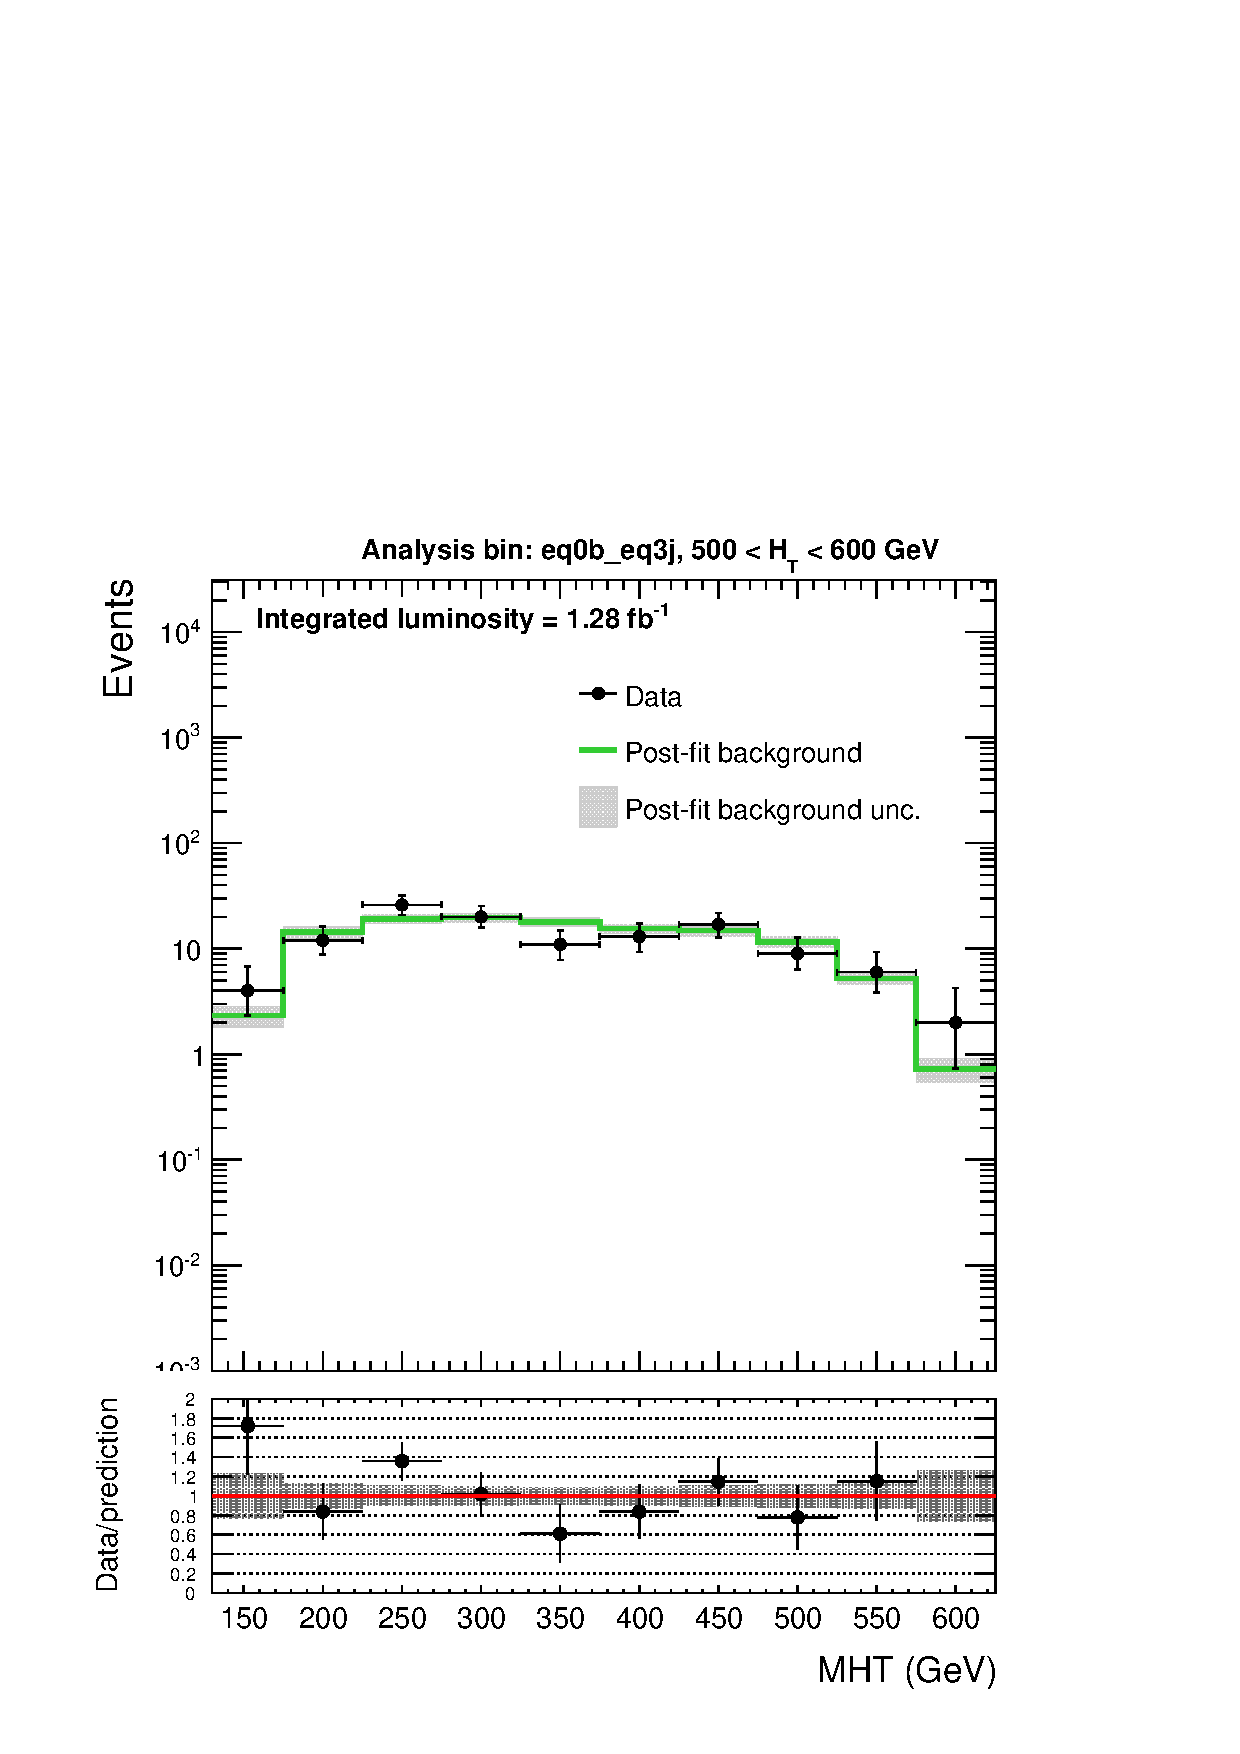
\includegraphics[width=0.25\textwidth]{figures/postFitResults/postFitShape_eq0b_eq3j_500_600.pdf} }\hspace{1cm}
    \subfigure[$\nj^{\mathrm{sym}}=3$, $\nb=0$, $600 < \scalht < 800 \; \mathrm{GeV}$]{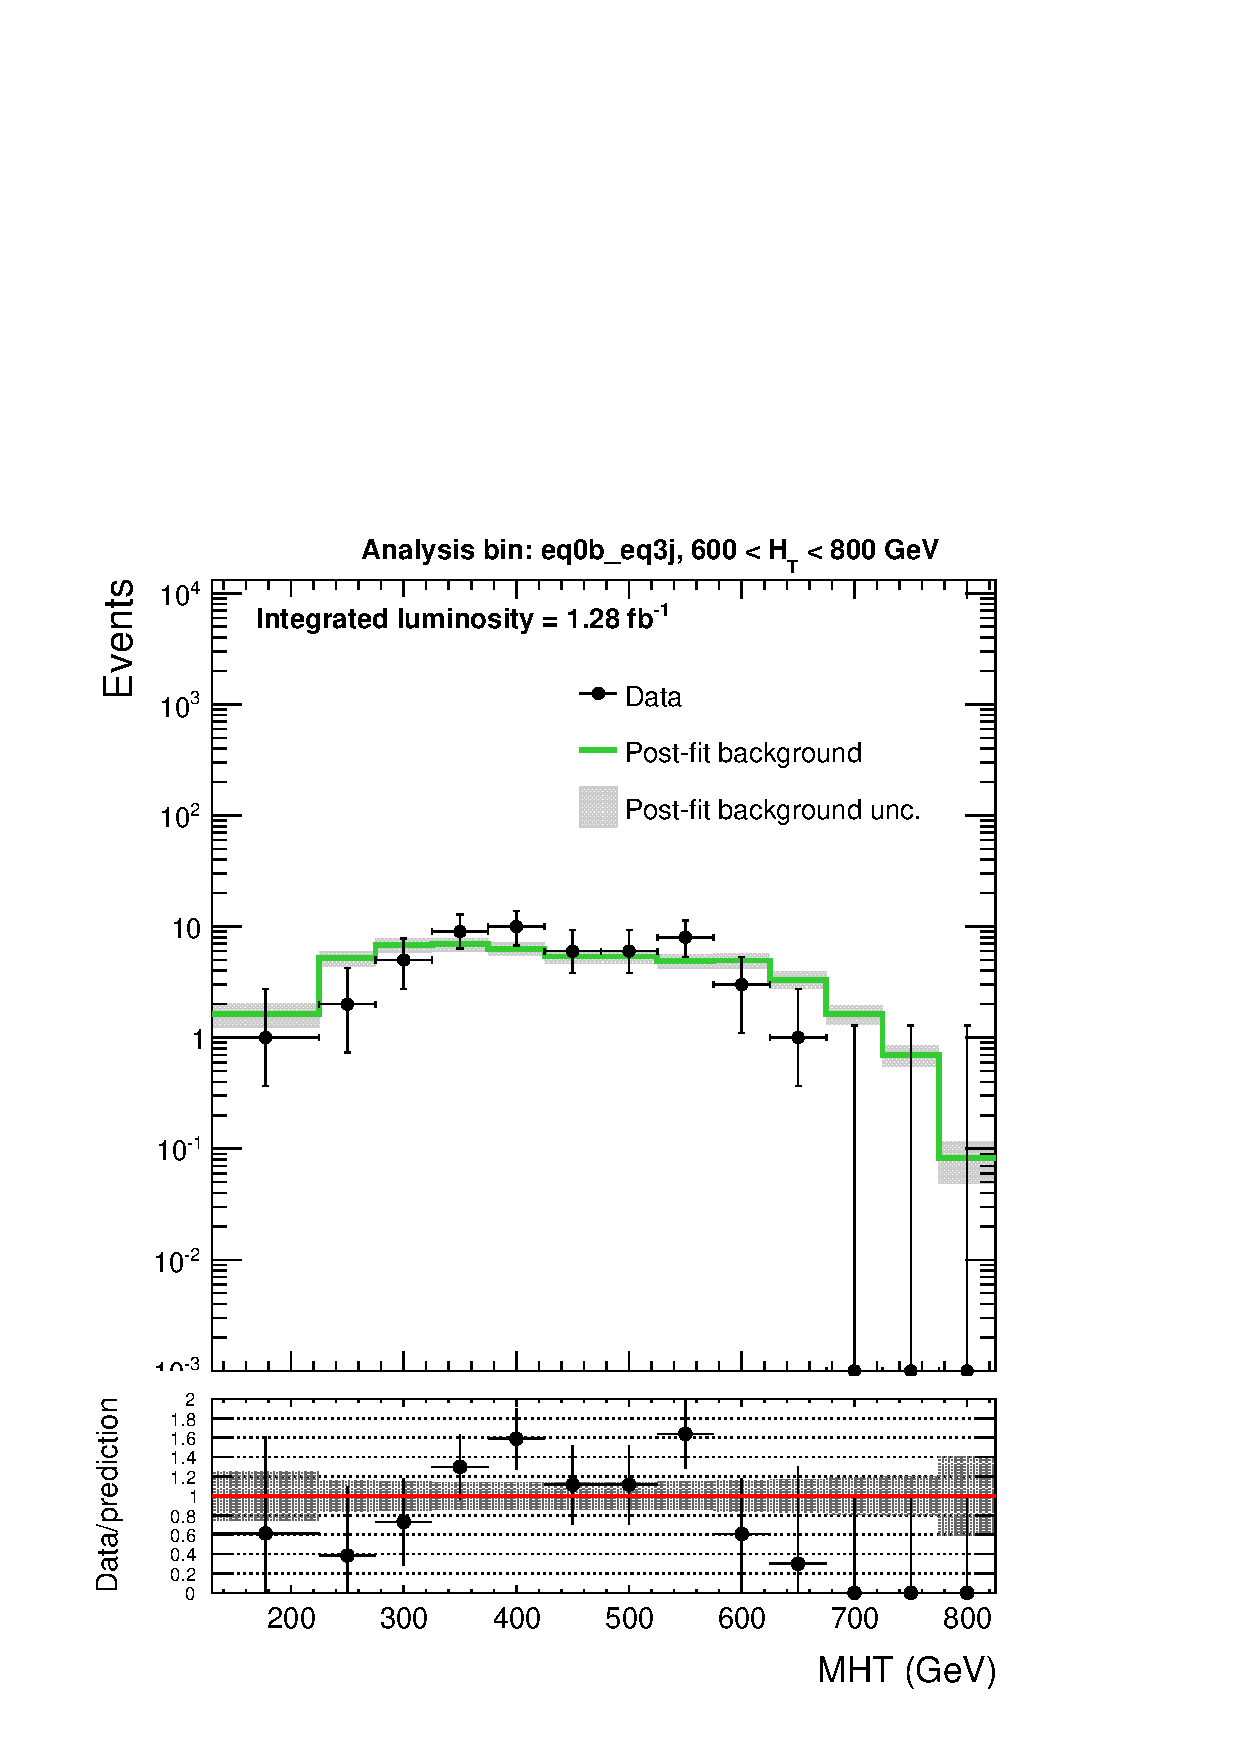
\includegraphics[width=0.25\textwidth]{figures/postFitResults/postFitShape_eq0b_eq3j_600_800.pdf} }\\
    \subfigure[$\nj^{\mathrm{sym}}=3$, $\nb=0$, $\scalht > 800 \; \mathrm{GeV}$]{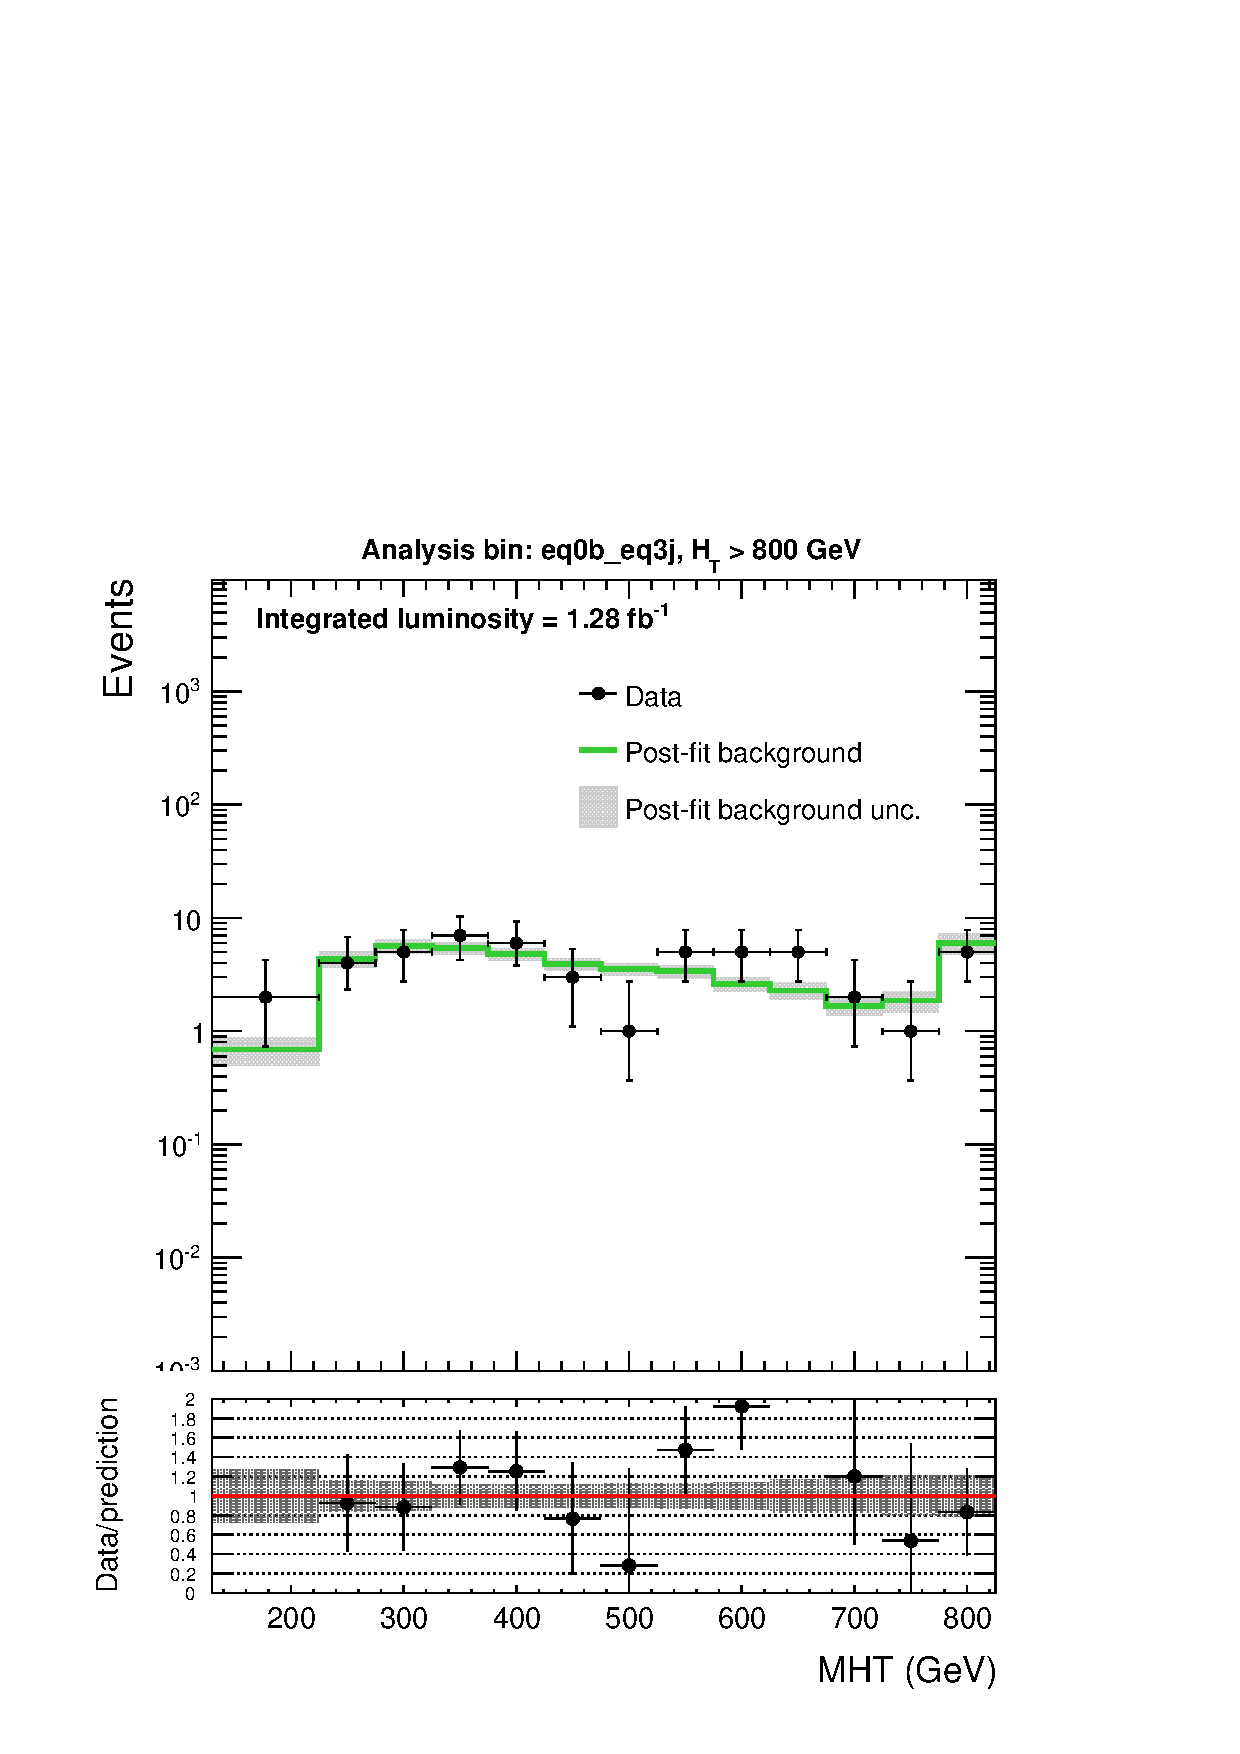
\includegraphics[width=0.25\textwidth]{figures/postFitResults/postFitShape_eq0b_eq3j_800_Inf.pdf} }\hspace{1cm}
  \end{center}
\end{figure}



\newpage
\begin{figure}[h!]
\caption{Post-fit \MHT templates for the bin $\nj^{\mathrm{asym}}=4$, $\nb=0$ \label{fig:postFitShapes_eq0b_eq4a}}.
\begin{center}

    \subfigure[$\nj^{\mathrm{asym}}=4$, $\nb=0$, $200 < \scalht < 250 \; \mathrm{GeV}$]{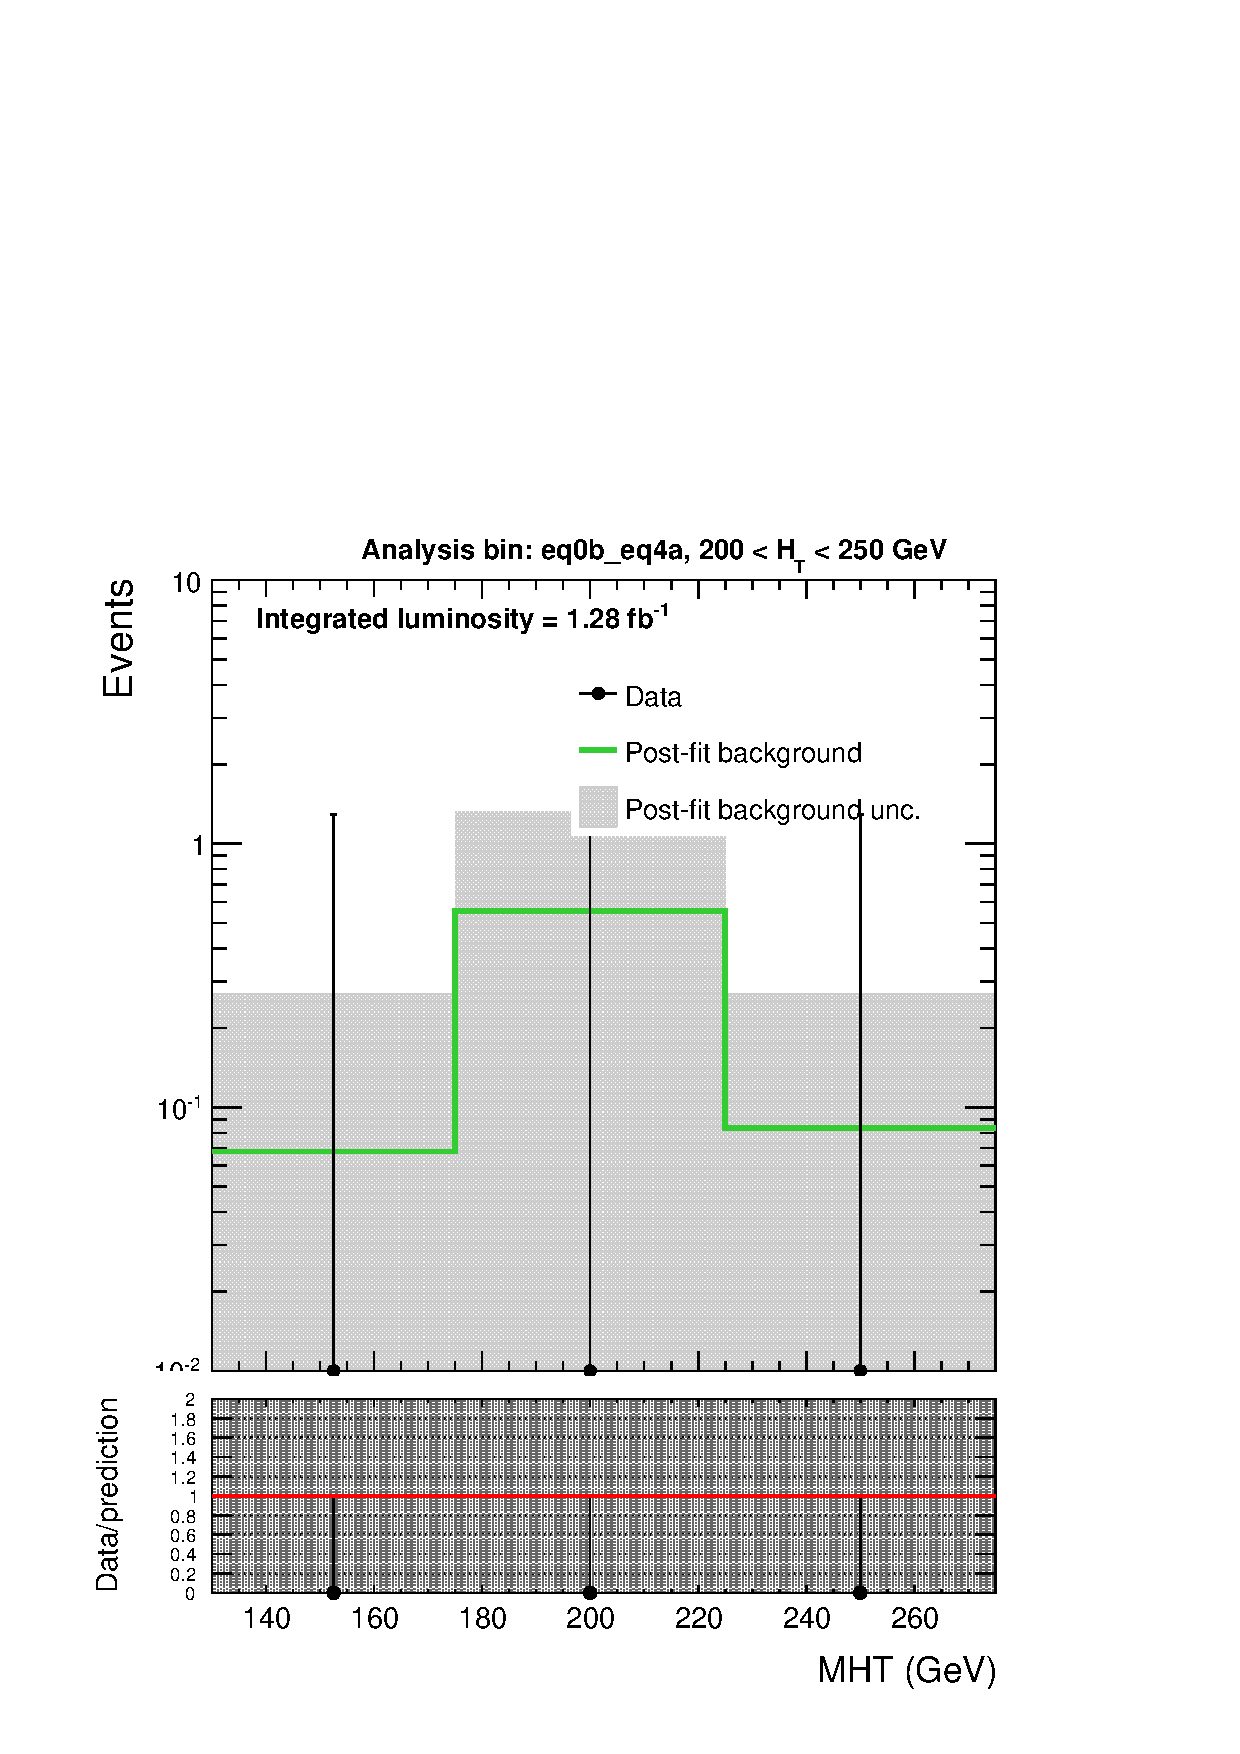
\includegraphics[width=0.25\textwidth]{figures/postFitResults/postFitShape_eq0b_eq4a_200_250.pdf} }\hspace{1cm}
    \subfigure[$\nj^{\mathrm{asym}}=4$, $\nb=0$, $250 < \scalht < 300 \; \mathrm{GeV}$]{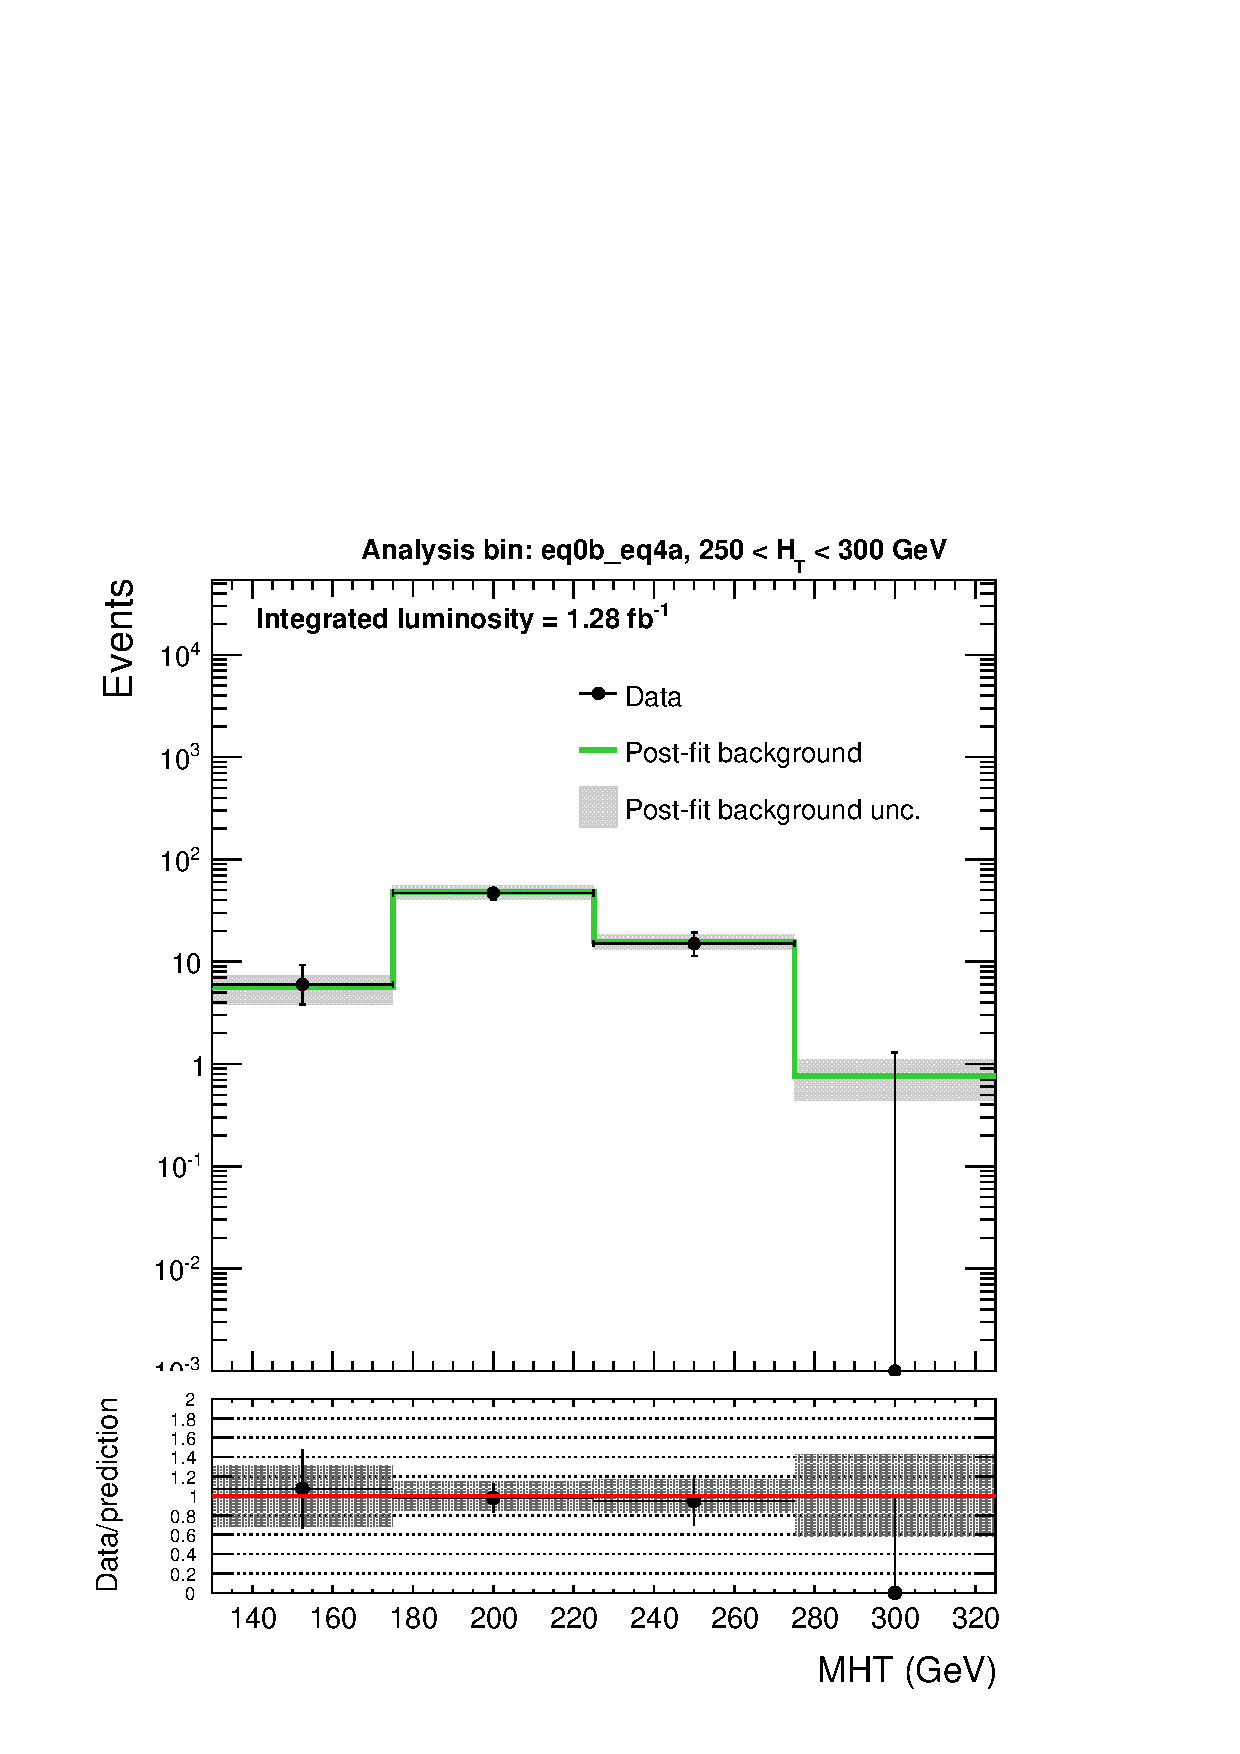
\includegraphics[width=0.25\textwidth]{figures/postFitResults/postFitShape_eq0b_eq4a_250_300.pdf} }\hspace{1cm}
    \subfigure[$\nj^{\mathrm{asym}}=4$, $\nb=0$, $300 < \scalht < 350 \; \mathrm{GeV}$]{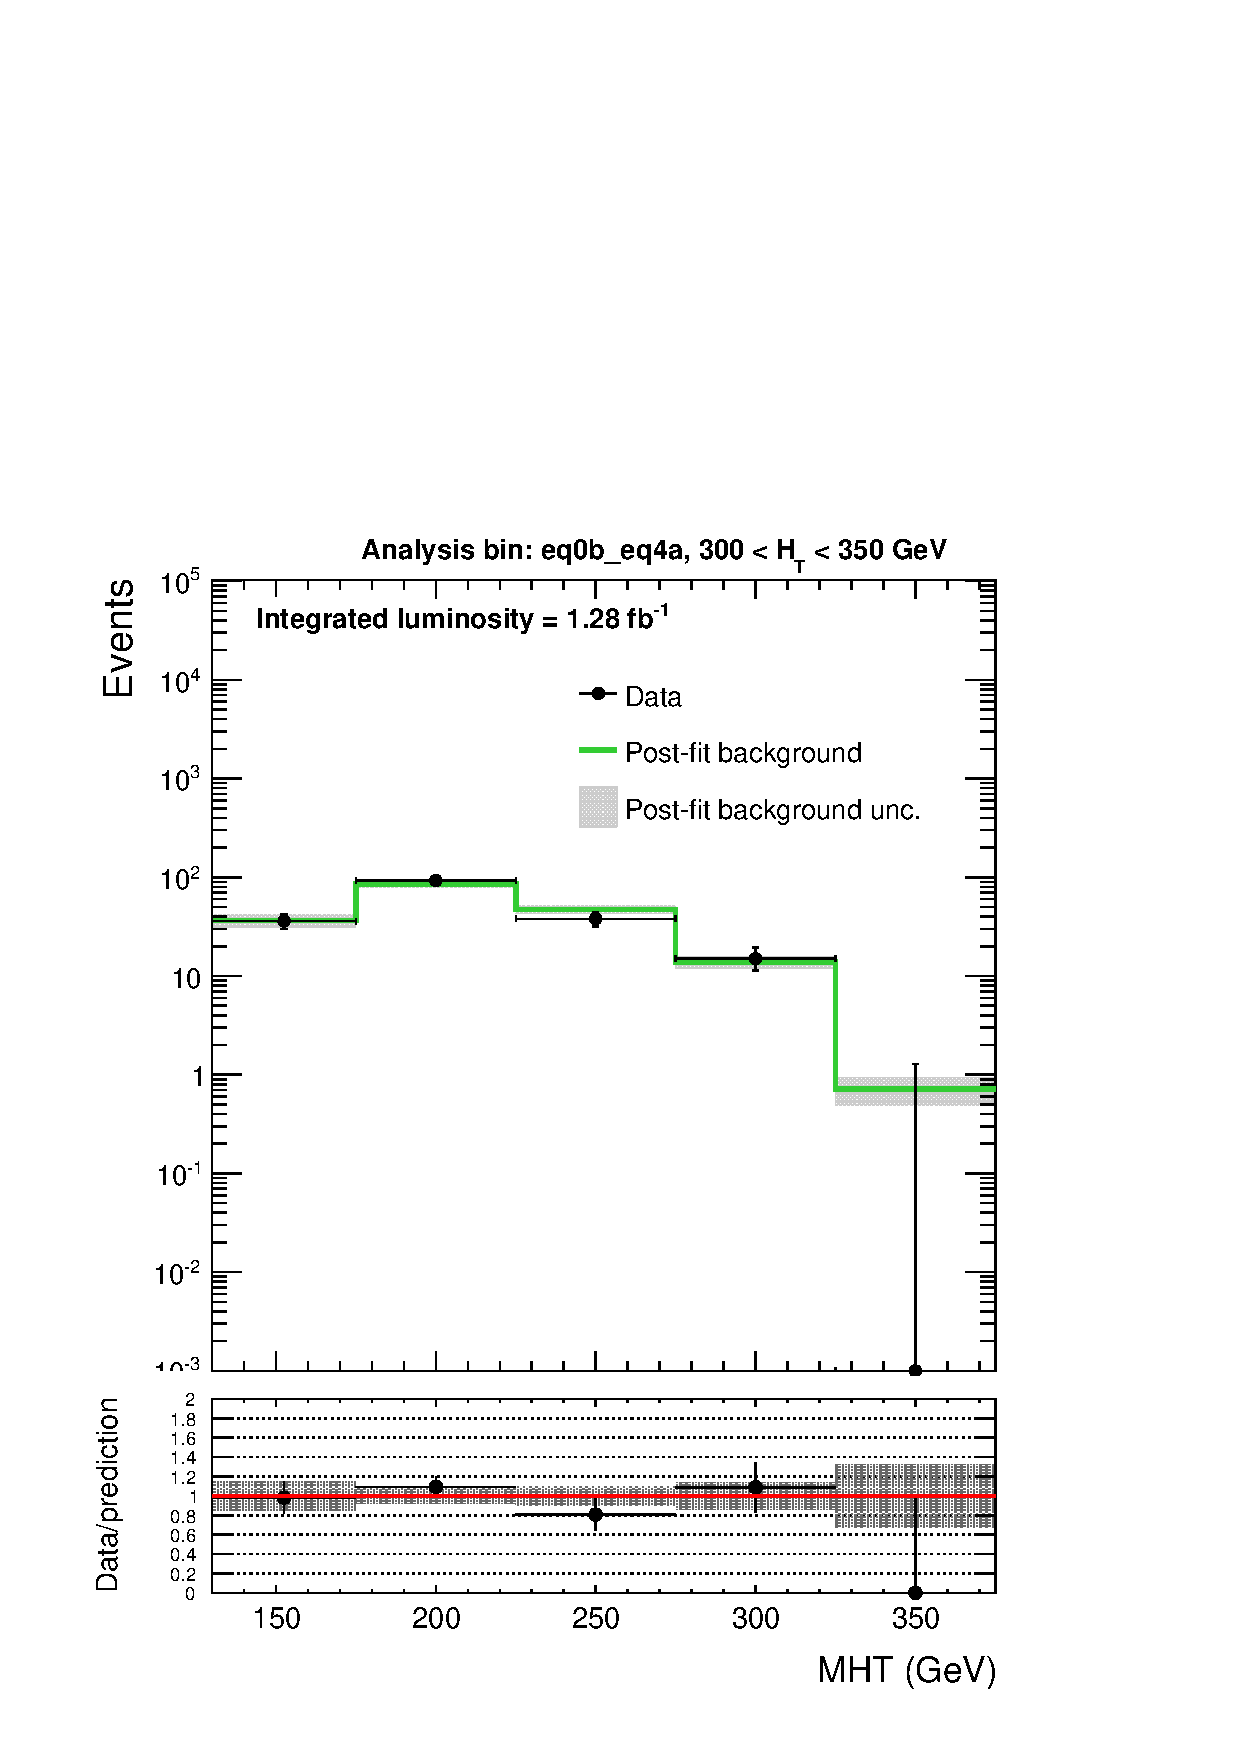
\includegraphics[width=0.25\textwidth]{figures/postFitResults/postFitShape_eq0b_eq4a_300_350.pdf} }\\
    \subfigure[$\nj^{\mathrm{asym}}=4$, $\nb=0$, $350 < \scalht < 400 \; \mathrm{GeV}$]{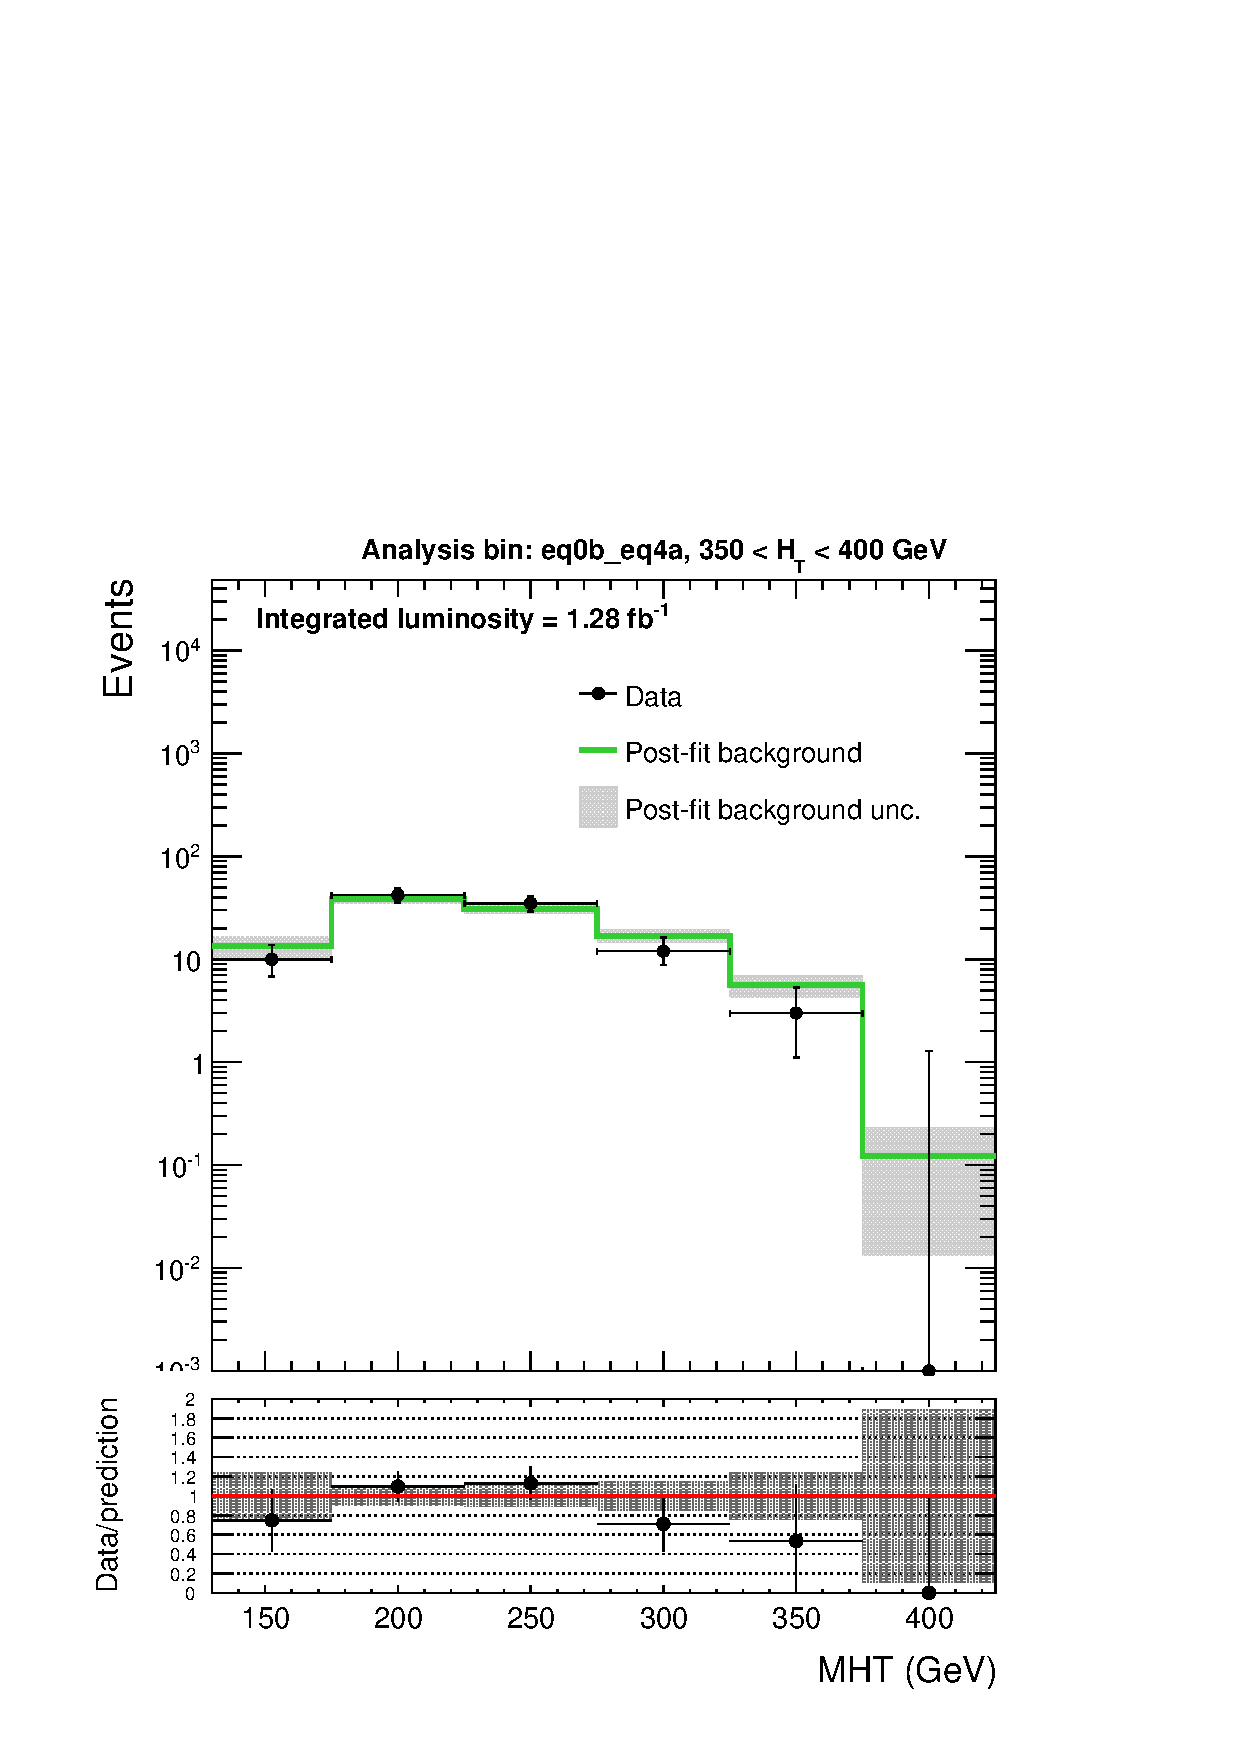
\includegraphics[width=0.25\textwidth]{figures/postFitResults/postFitShape_eq0b_eq4a_350_400.pdf} }\hspace{1cm}
    \subfigure[$\nj^{\mathrm{asym}}=4$, $\nb=0$, $400 < \scalht < 500 \; \mathrm{GeV}$]{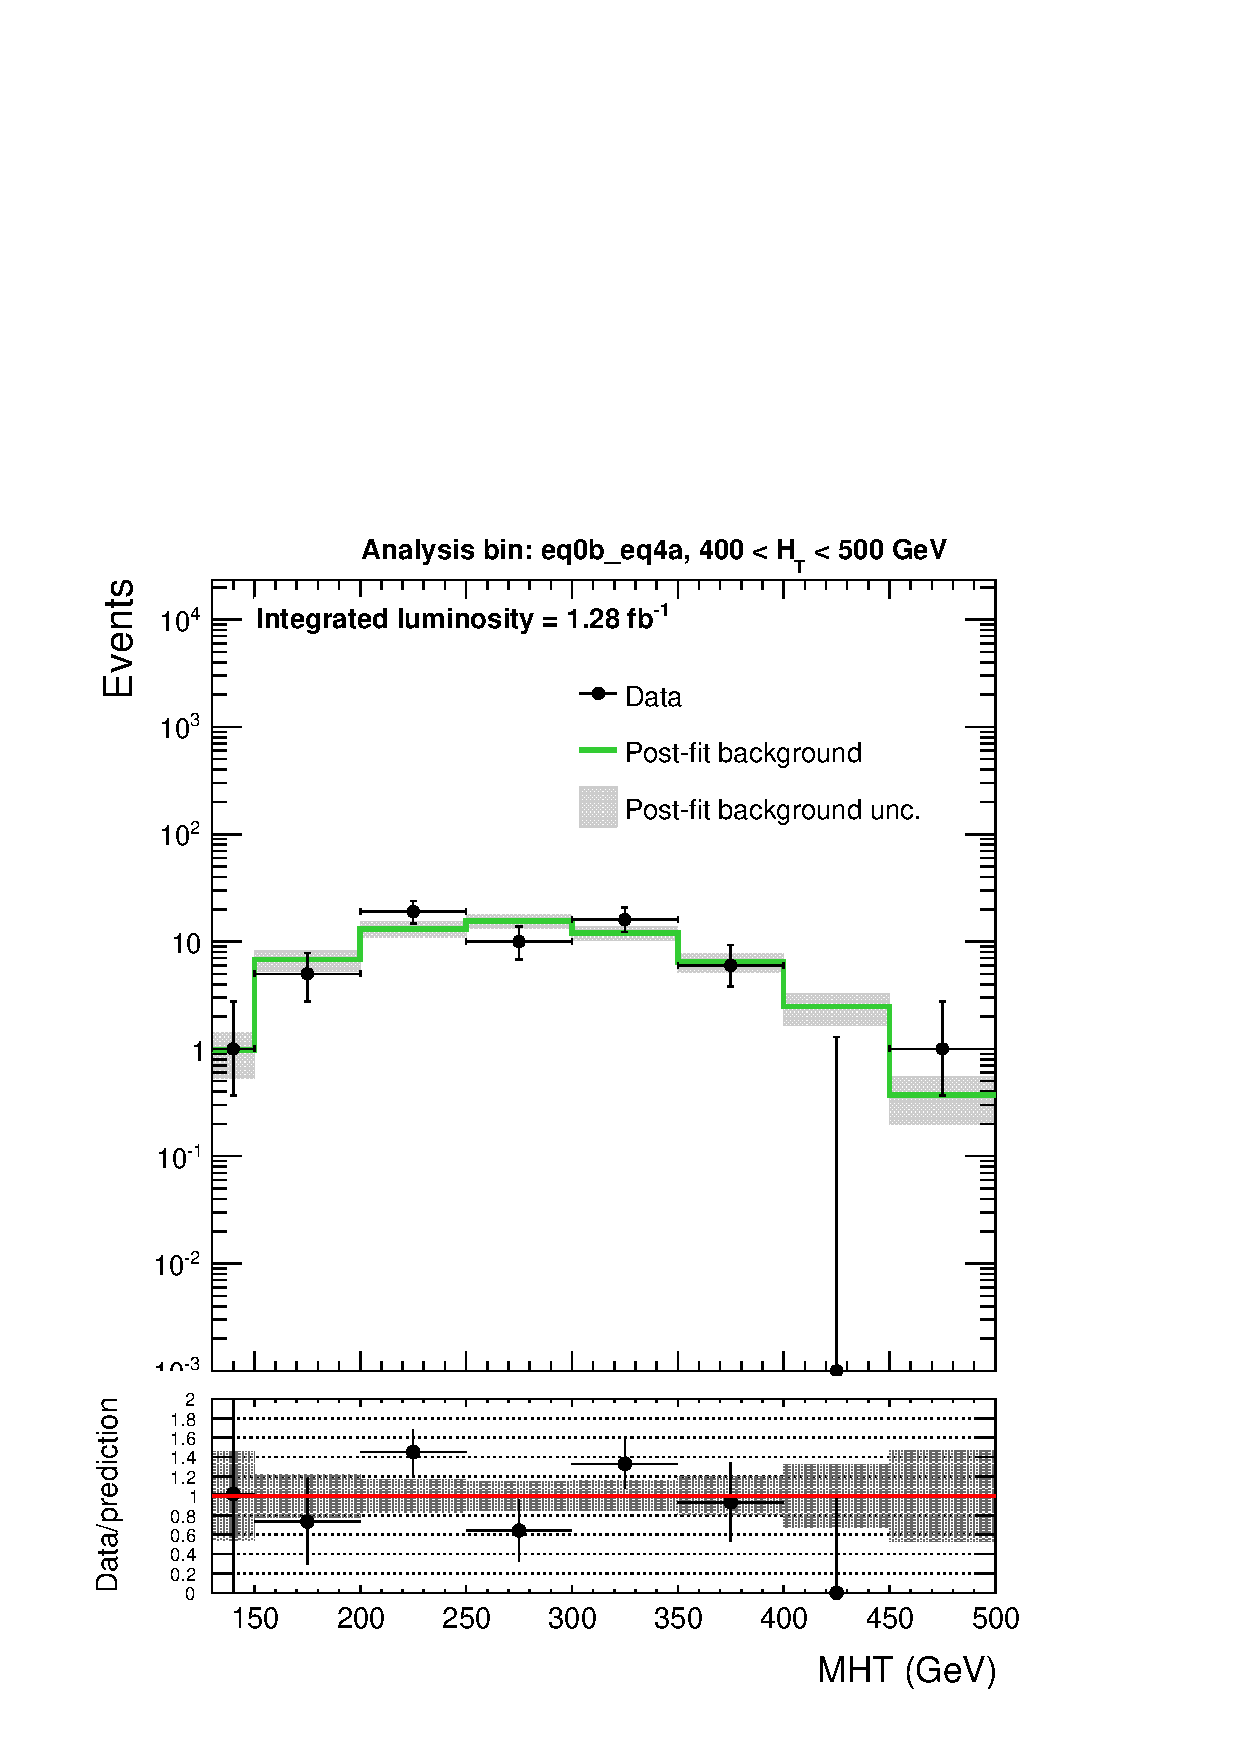
\includegraphics[width=0.25\textwidth]{figures/postFitResults/postFitShape_eq0b_eq4a_400_500.pdf} }\hspace{1cm}
    \subfigure[$\nj^{\mathrm{asym}}=4$, $\nb=0$, $500 < \scalht < 600 \; \mathrm{GeV}$]{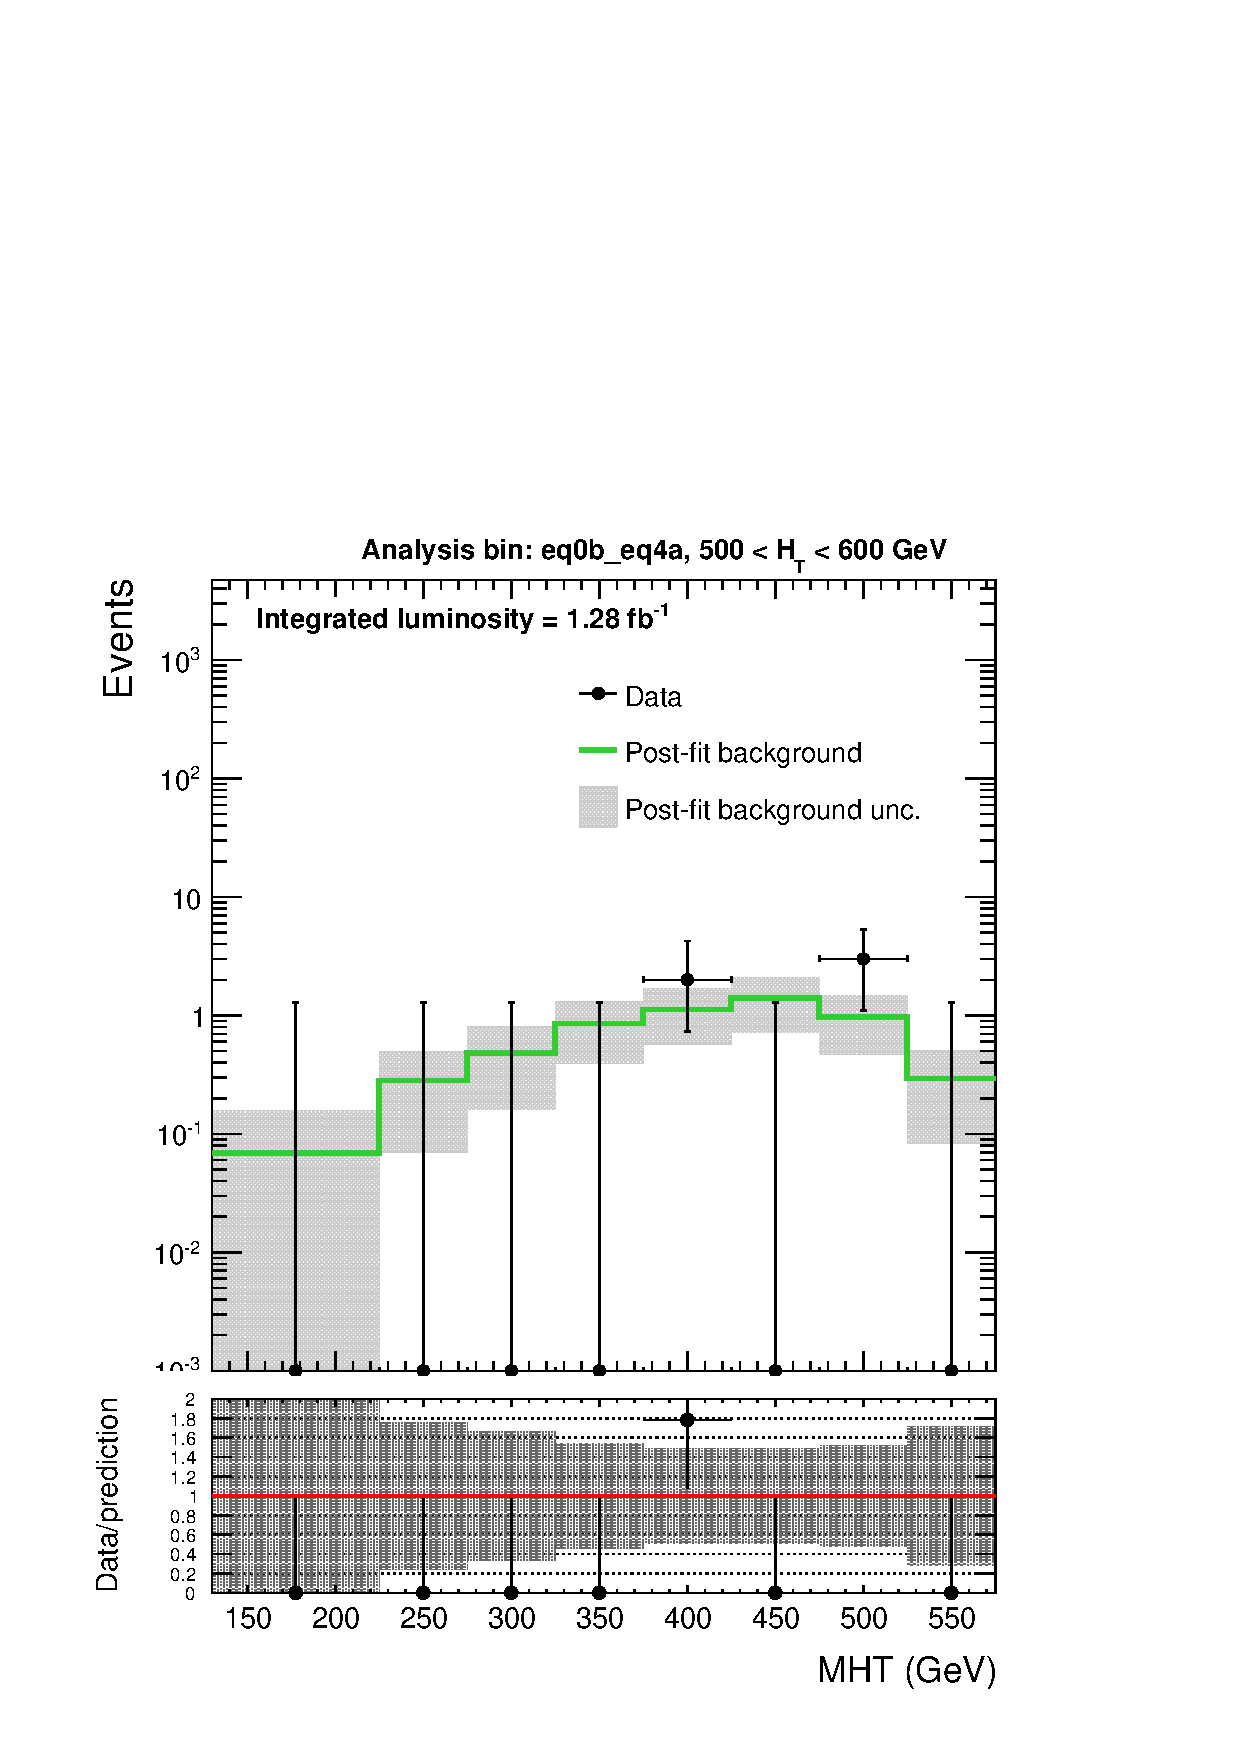
\includegraphics[width=0.25\textwidth]{figures/postFitResults/postFitShape_eq0b_eq4a_500_600.pdf} }\\
    \subfigure[$\nj^{\mathrm{asym}}=4$, $\nb=0$, $\scalht > 600 \; \mathrm{GeV}$]{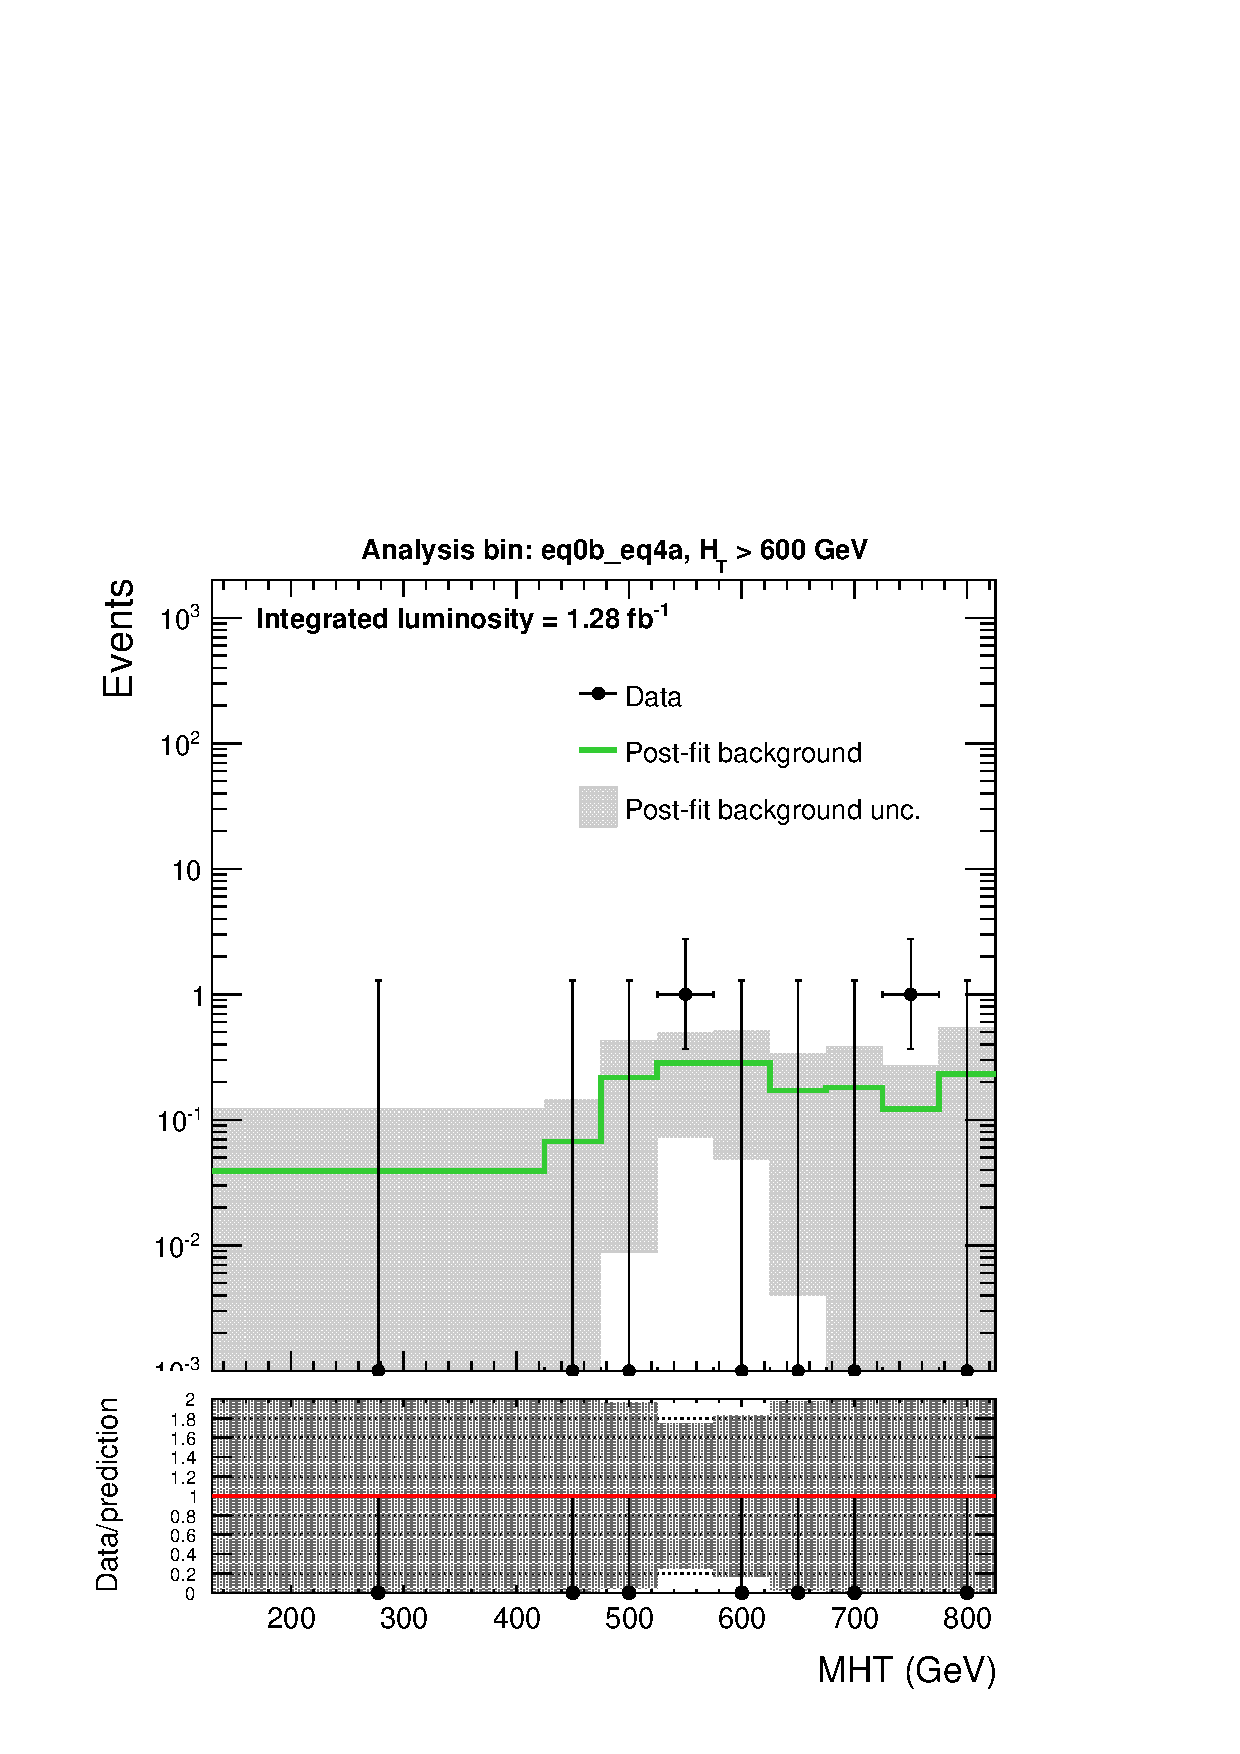
\includegraphics[width=0.25\textwidth]{figures/postFitResults/postFitShape_eq0b_eq4a_600_Inf.pdf} }\hspace{1cm}
  \end{center}
\end{figure}



\newpage
\begin{figure}[h!]
\caption{Post-fit \MHT templates for the bin $\nj^{\mathrm{sym}}=4$, $\nb=0$ \label{fig:postFitShapes_eq0b_eq4j}}.
\begin{center}

    \subfigure[$\nj^{\mathrm{sym}}=4$, $\nb=0$, $300 < \scalht < 350 \; \mathrm{GeV}$]{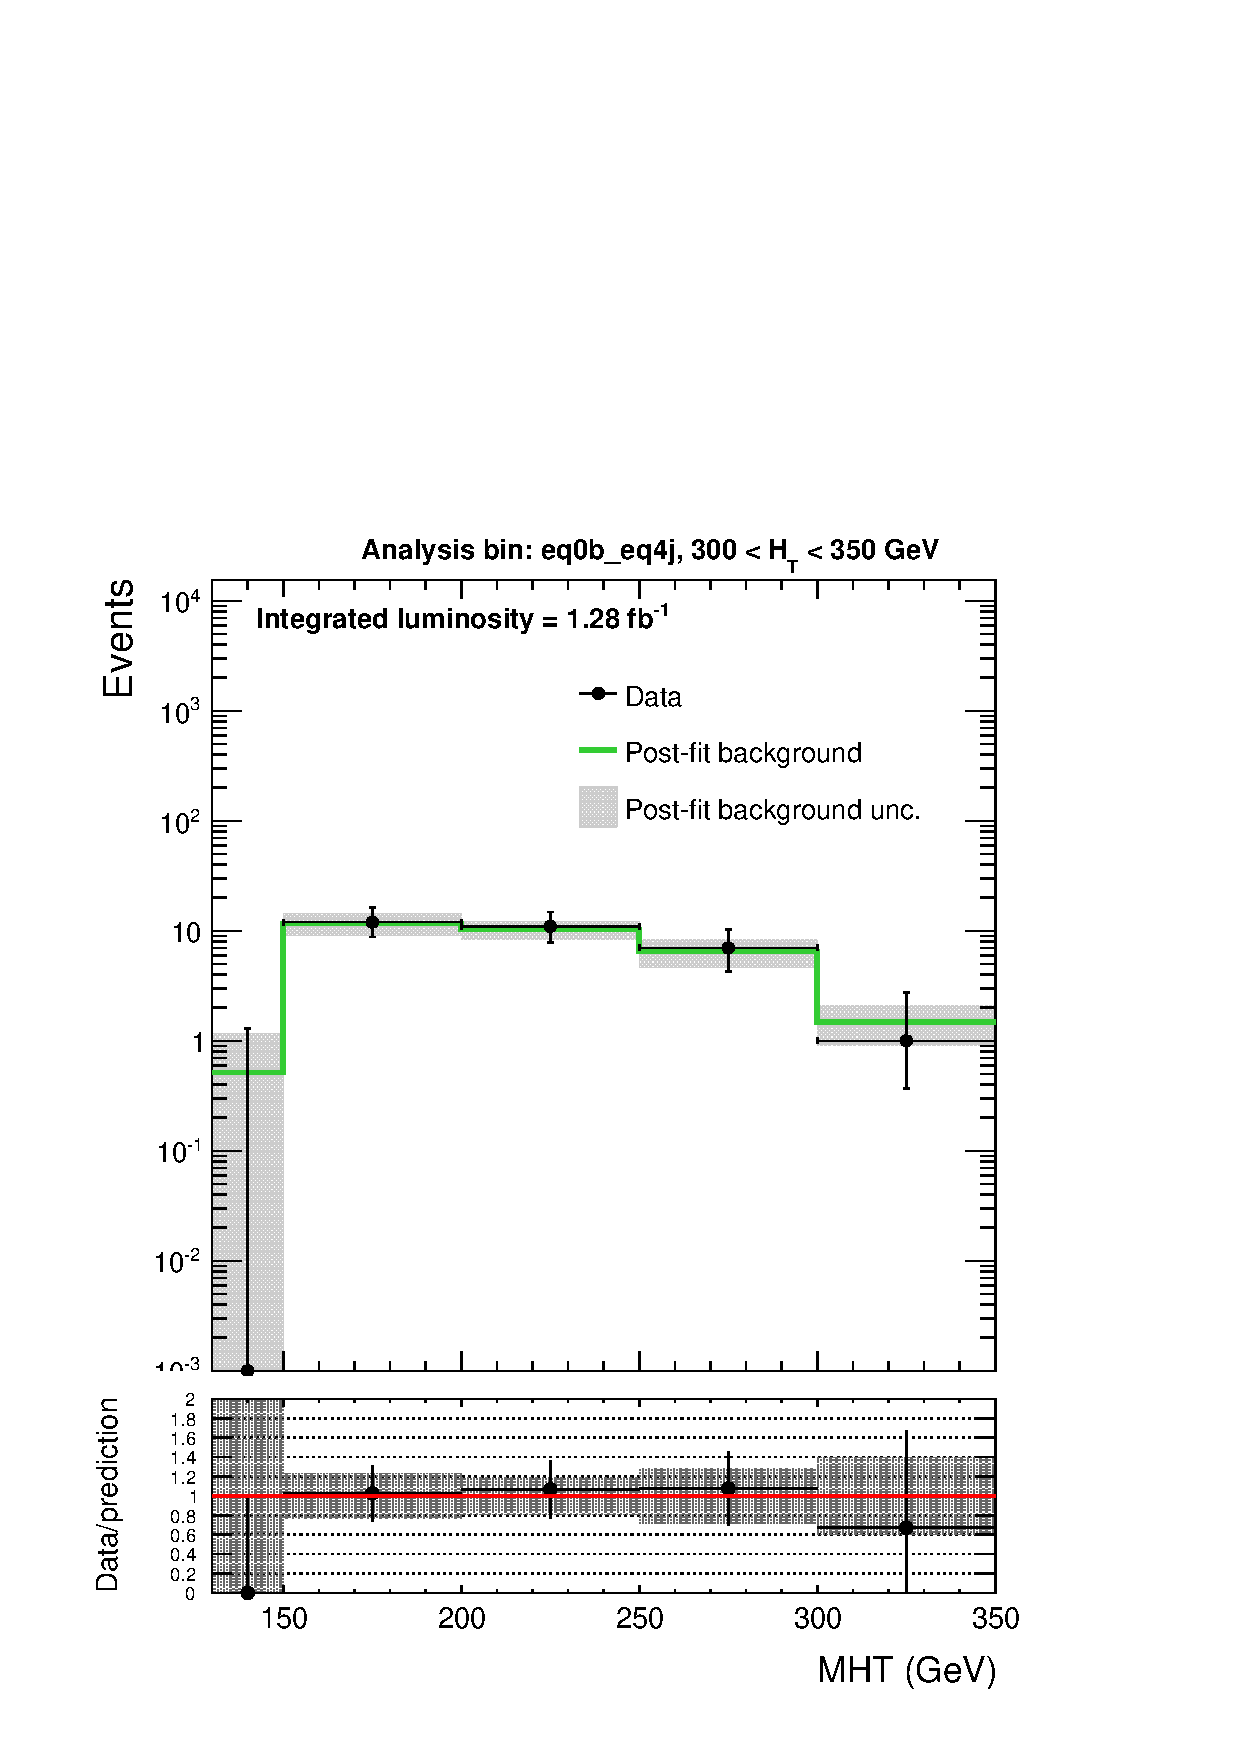
\includegraphics[width=0.25\textwidth]{figures/postFitResults/postFitShape_eq0b_eq4j_300_350.pdf} }\hspace{1cm}
    \subfigure[$\nj^{\mathrm{sym}}=4$, $\nb=0$, $350 < \scalht < 400 \; \mathrm{GeV}$]{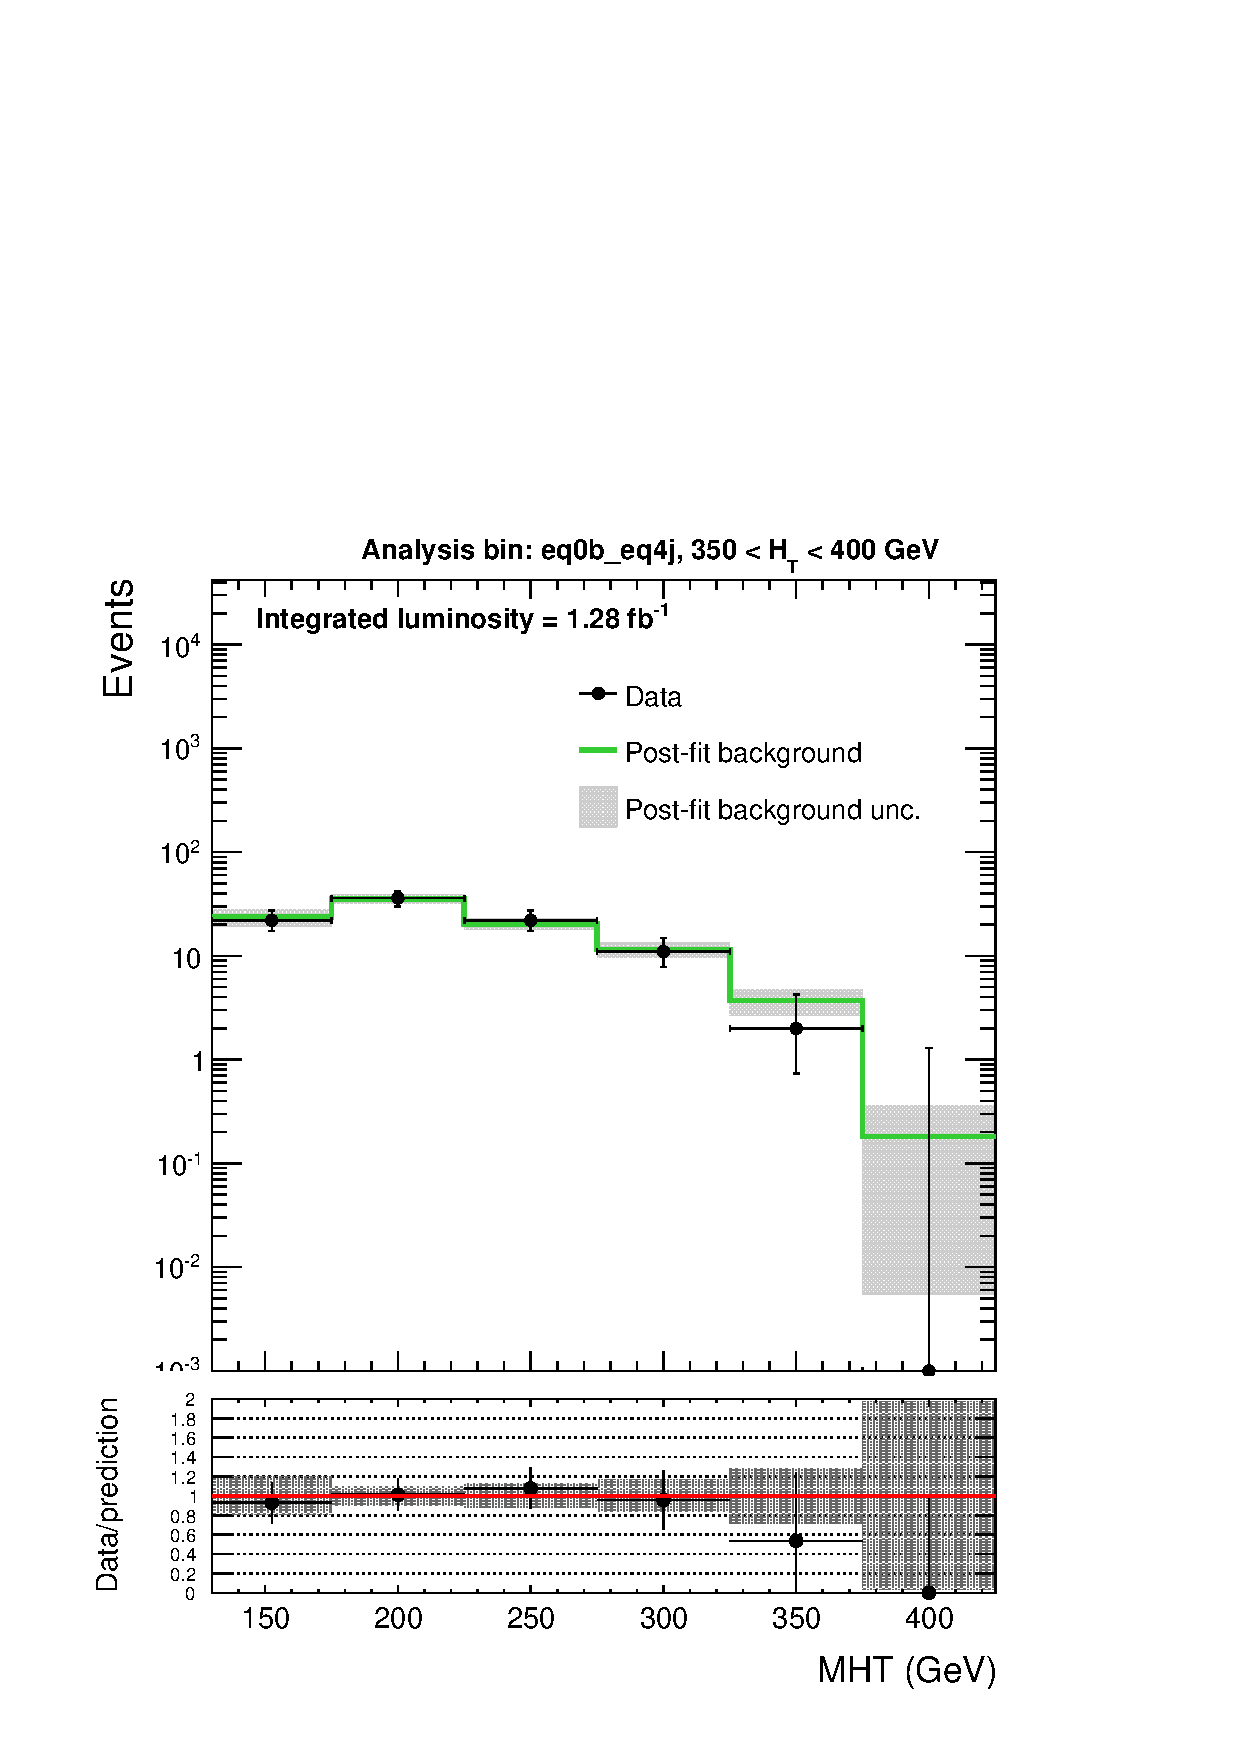
\includegraphics[width=0.25\textwidth]{figures/postFitResults/postFitShape_eq0b_eq4j_350_400.pdf} }\hspace{1cm}
    \subfigure[$\nj^{\mathrm{sym}}=4$, $\nb=0$, $400 < \scalht < 500 \; \mathrm{GeV}$]{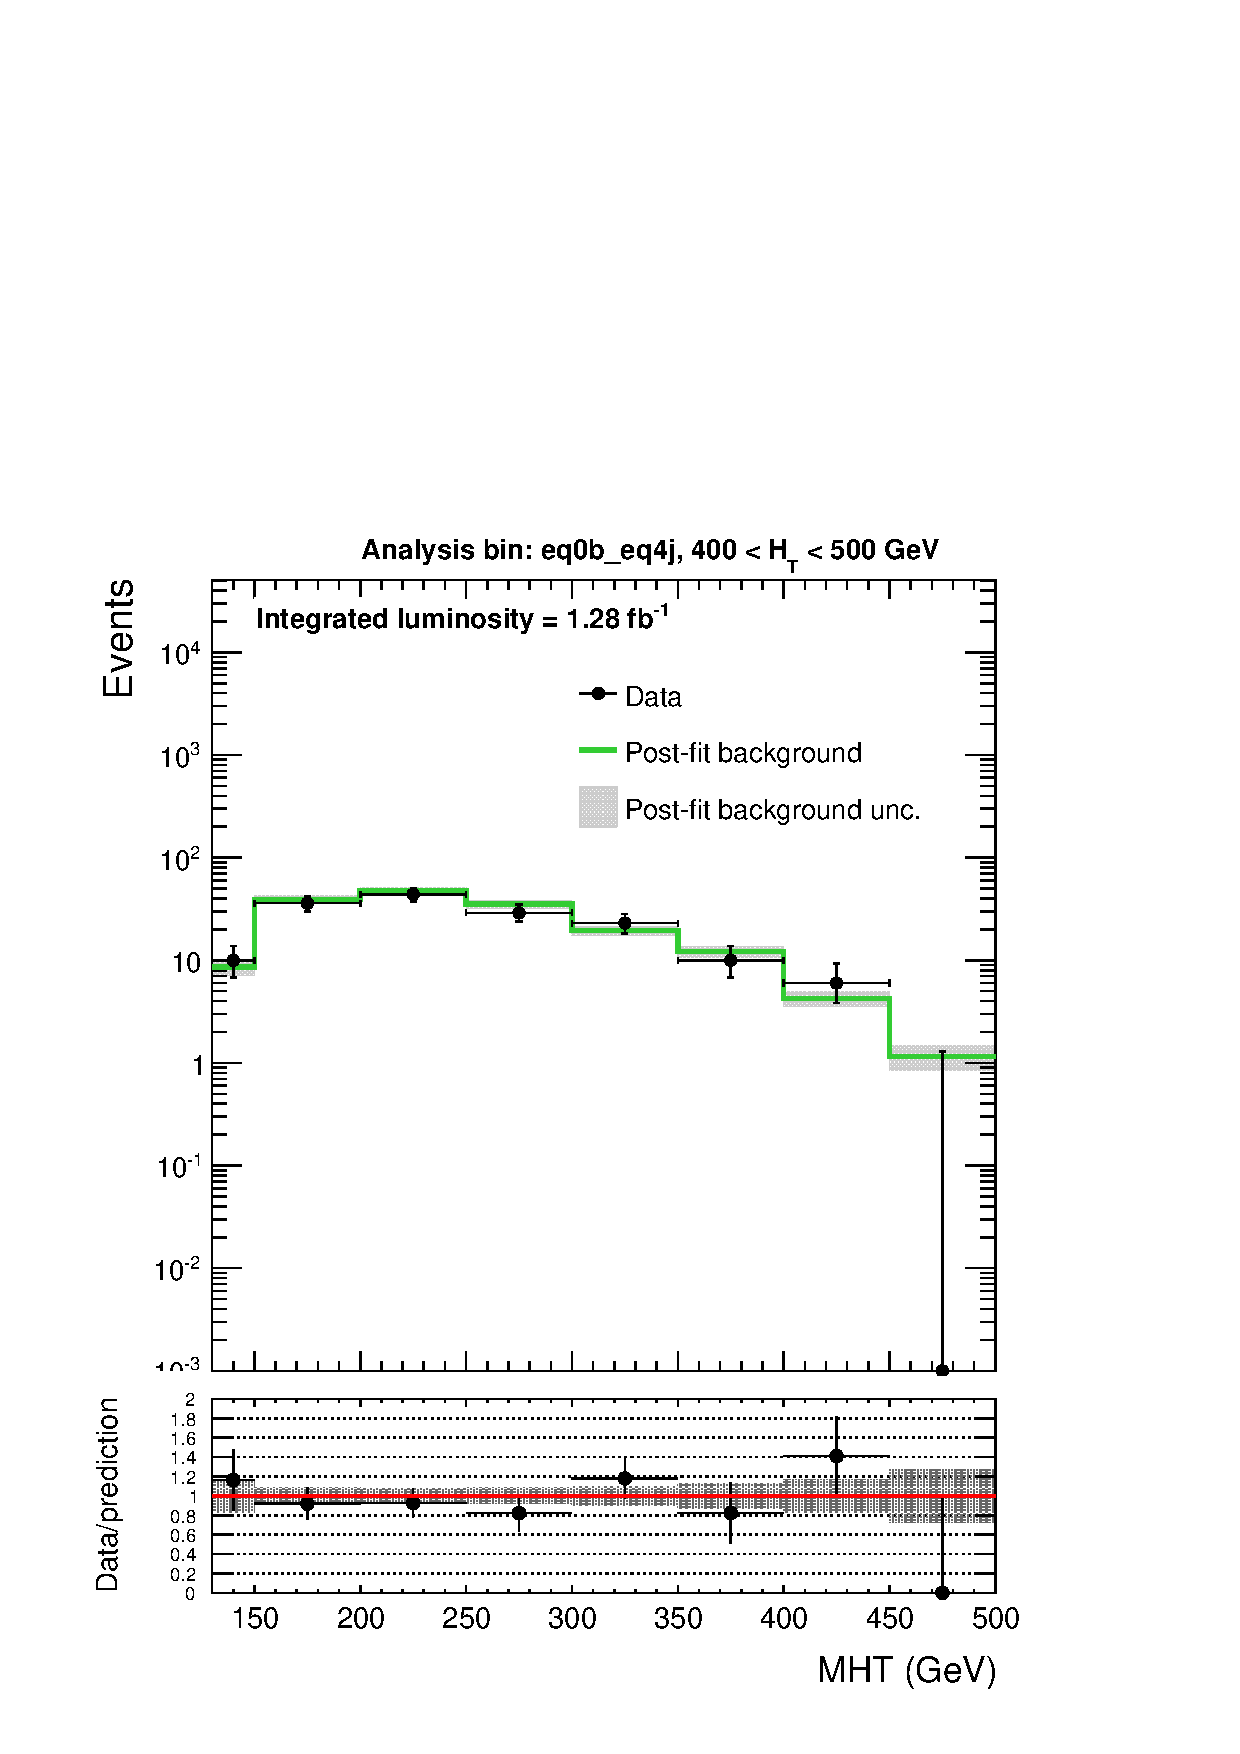
\includegraphics[width=0.25\textwidth]{figures/postFitResults/postFitShape_eq0b_eq4j_400_500.pdf} }\\
    \subfigure[$\nj^{\mathrm{sym}}=4$, $\nb=0$, $500 < \scalht < 600 \; \mathrm{GeV}$]{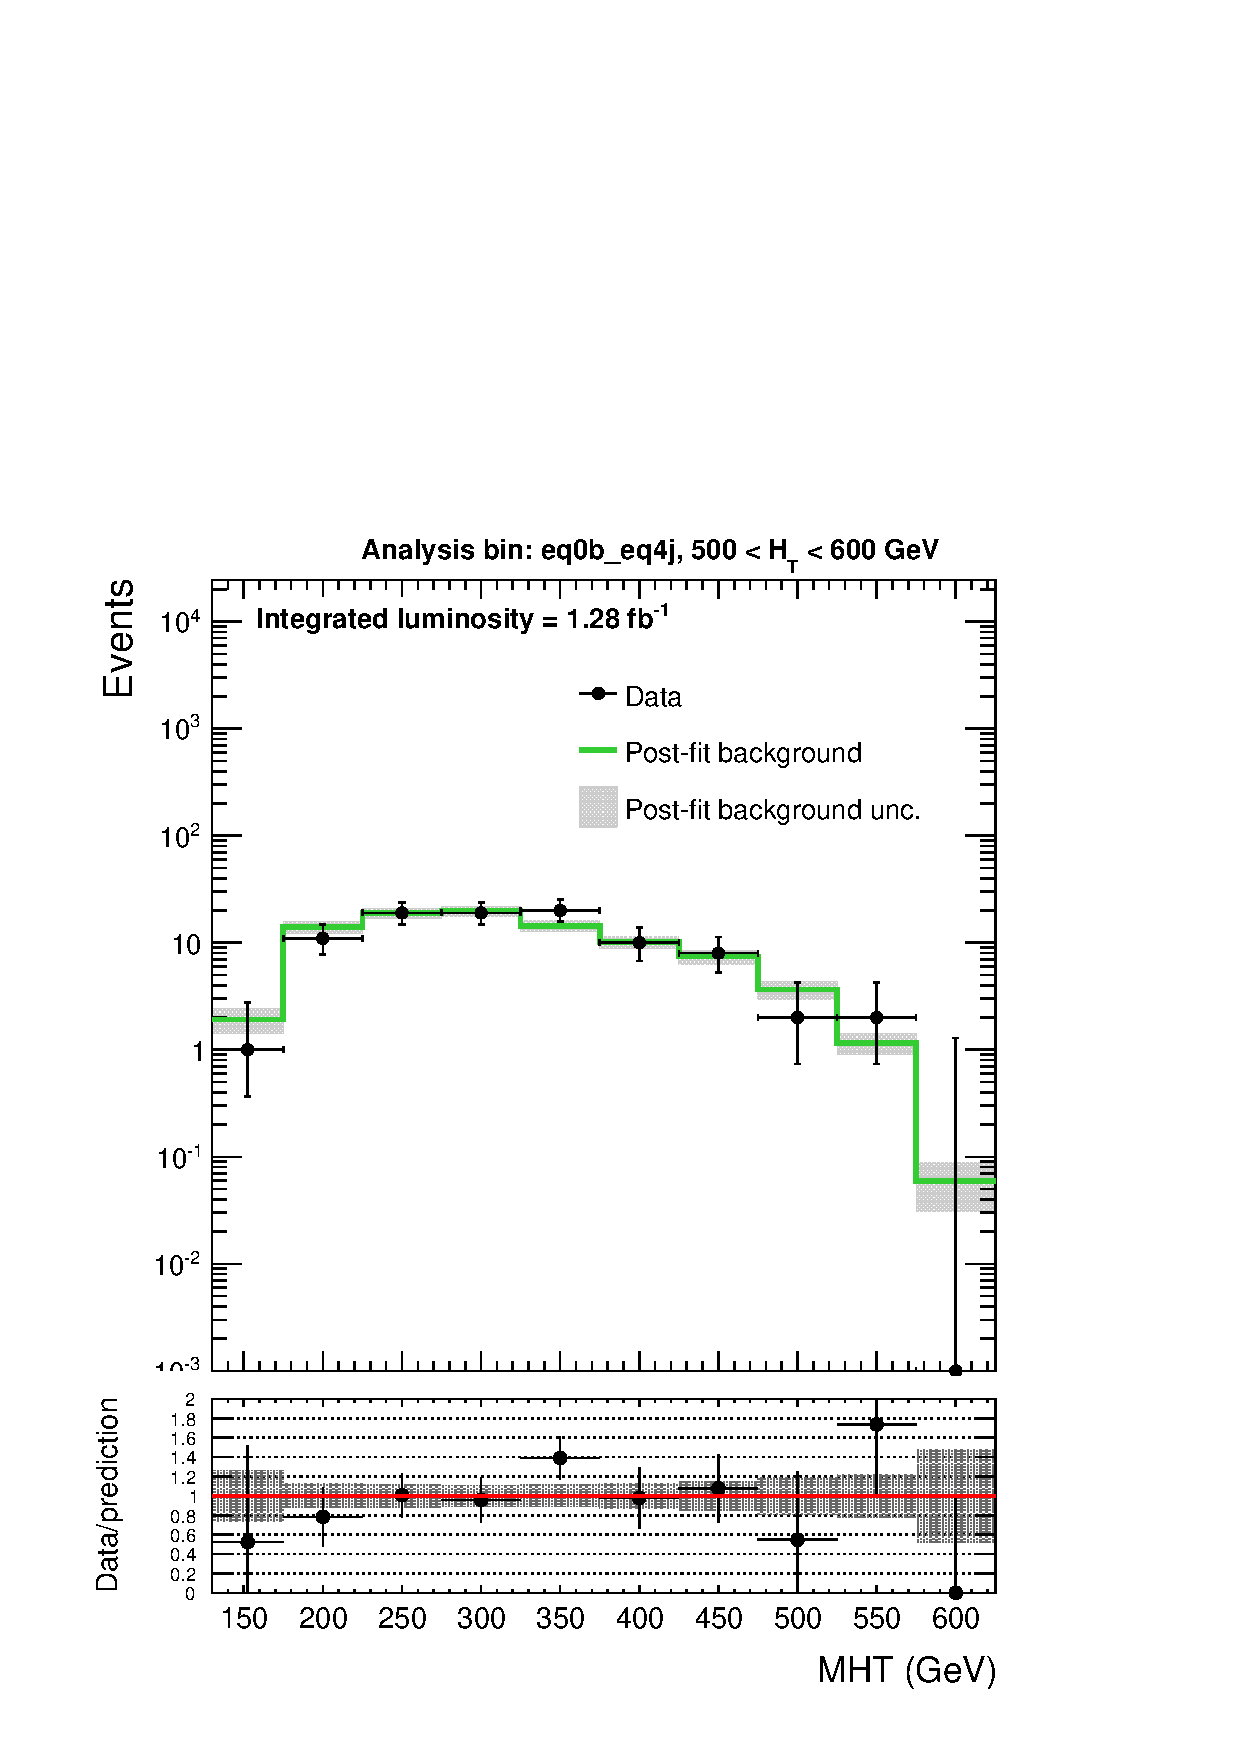
\includegraphics[width=0.25\textwidth]{figures/postFitResults/postFitShape_eq0b_eq4j_500_600.pdf} }\hspace{1cm}
    \subfigure[$\nj^{\mathrm{sym}}=4$, $\nb=0$, $600 < \scalht < 800 \; \mathrm{GeV}$]{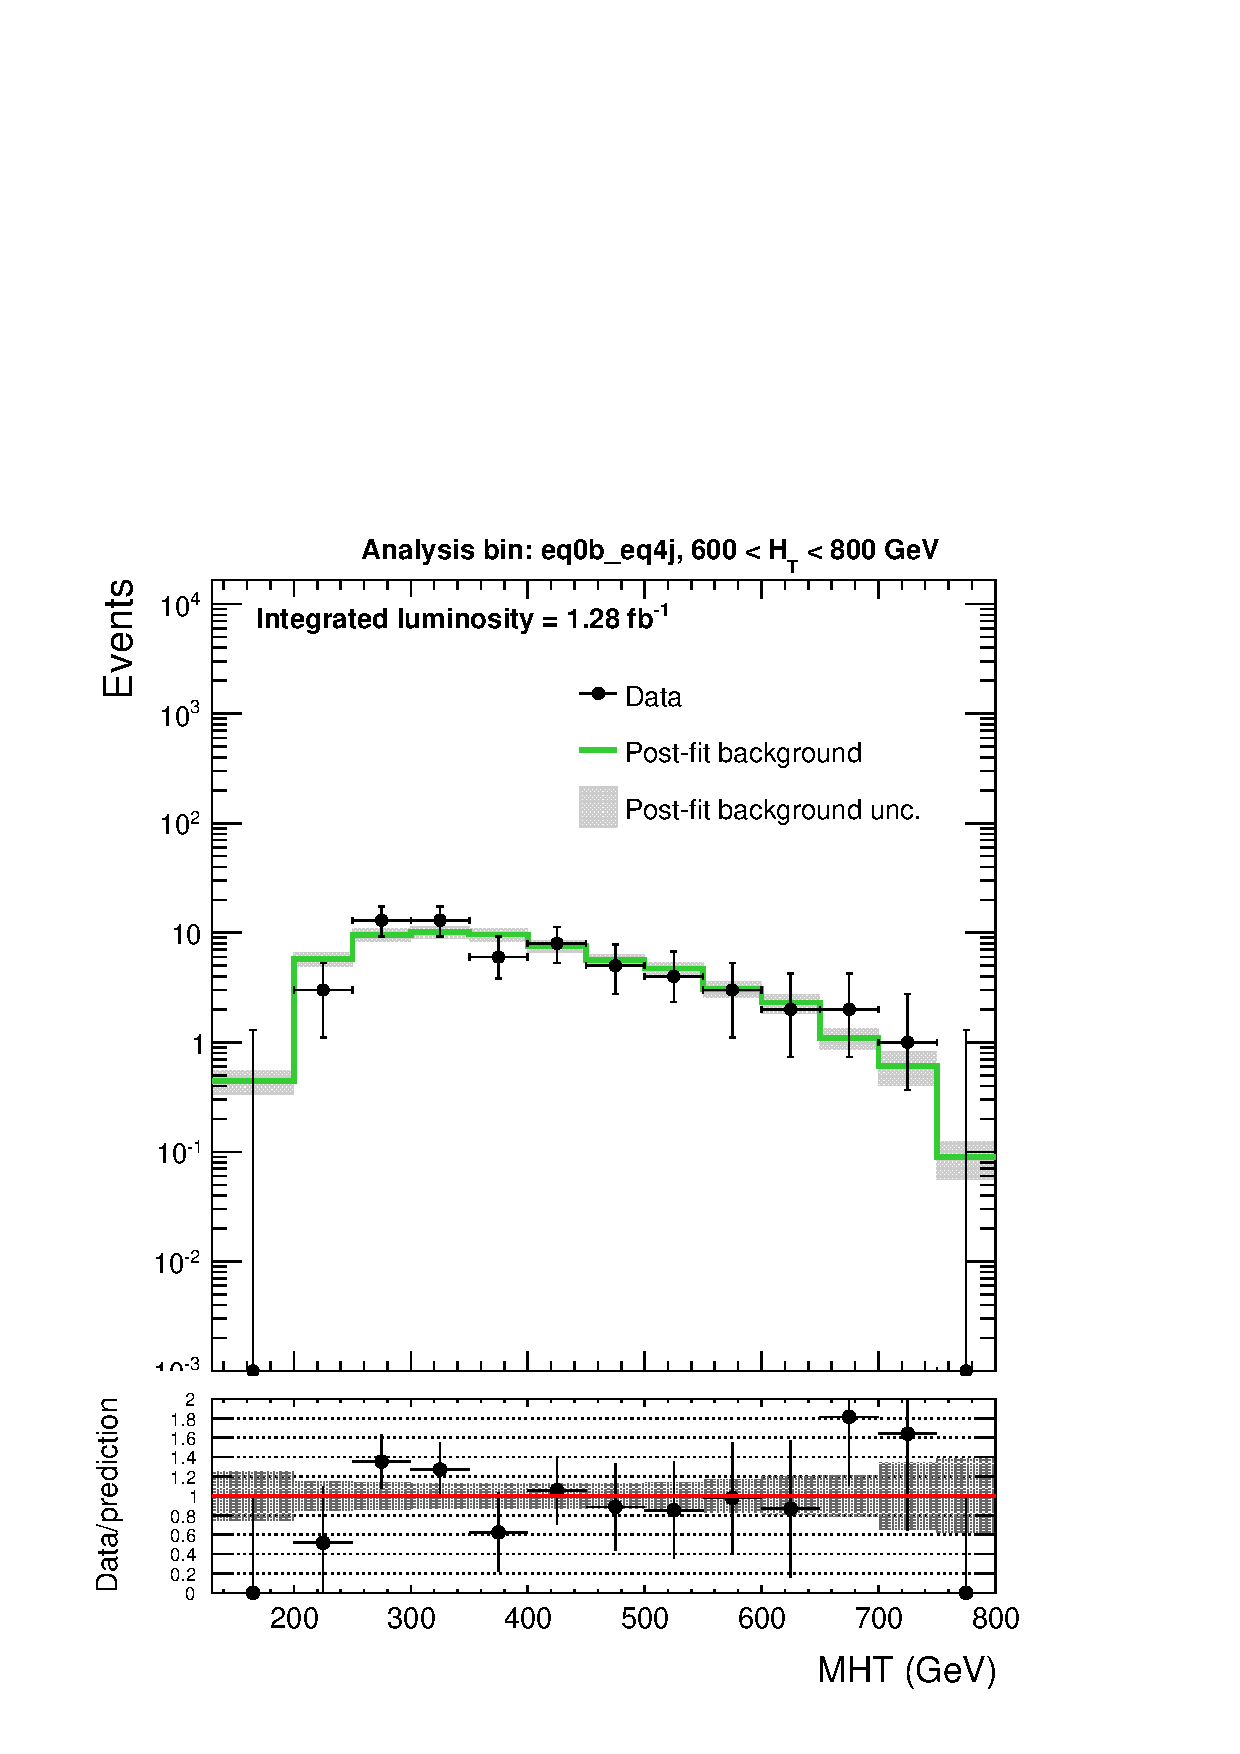
\includegraphics[width=0.25\textwidth]{figures/postFitResults/postFitShape_eq0b_eq4j_600_800.pdf} }\hspace{1cm}
    \subfigure[$\nj^{\mathrm{sym}}=4$, $\nb=0$, $\scalht > 800 \; \mathrm{GeV}$]{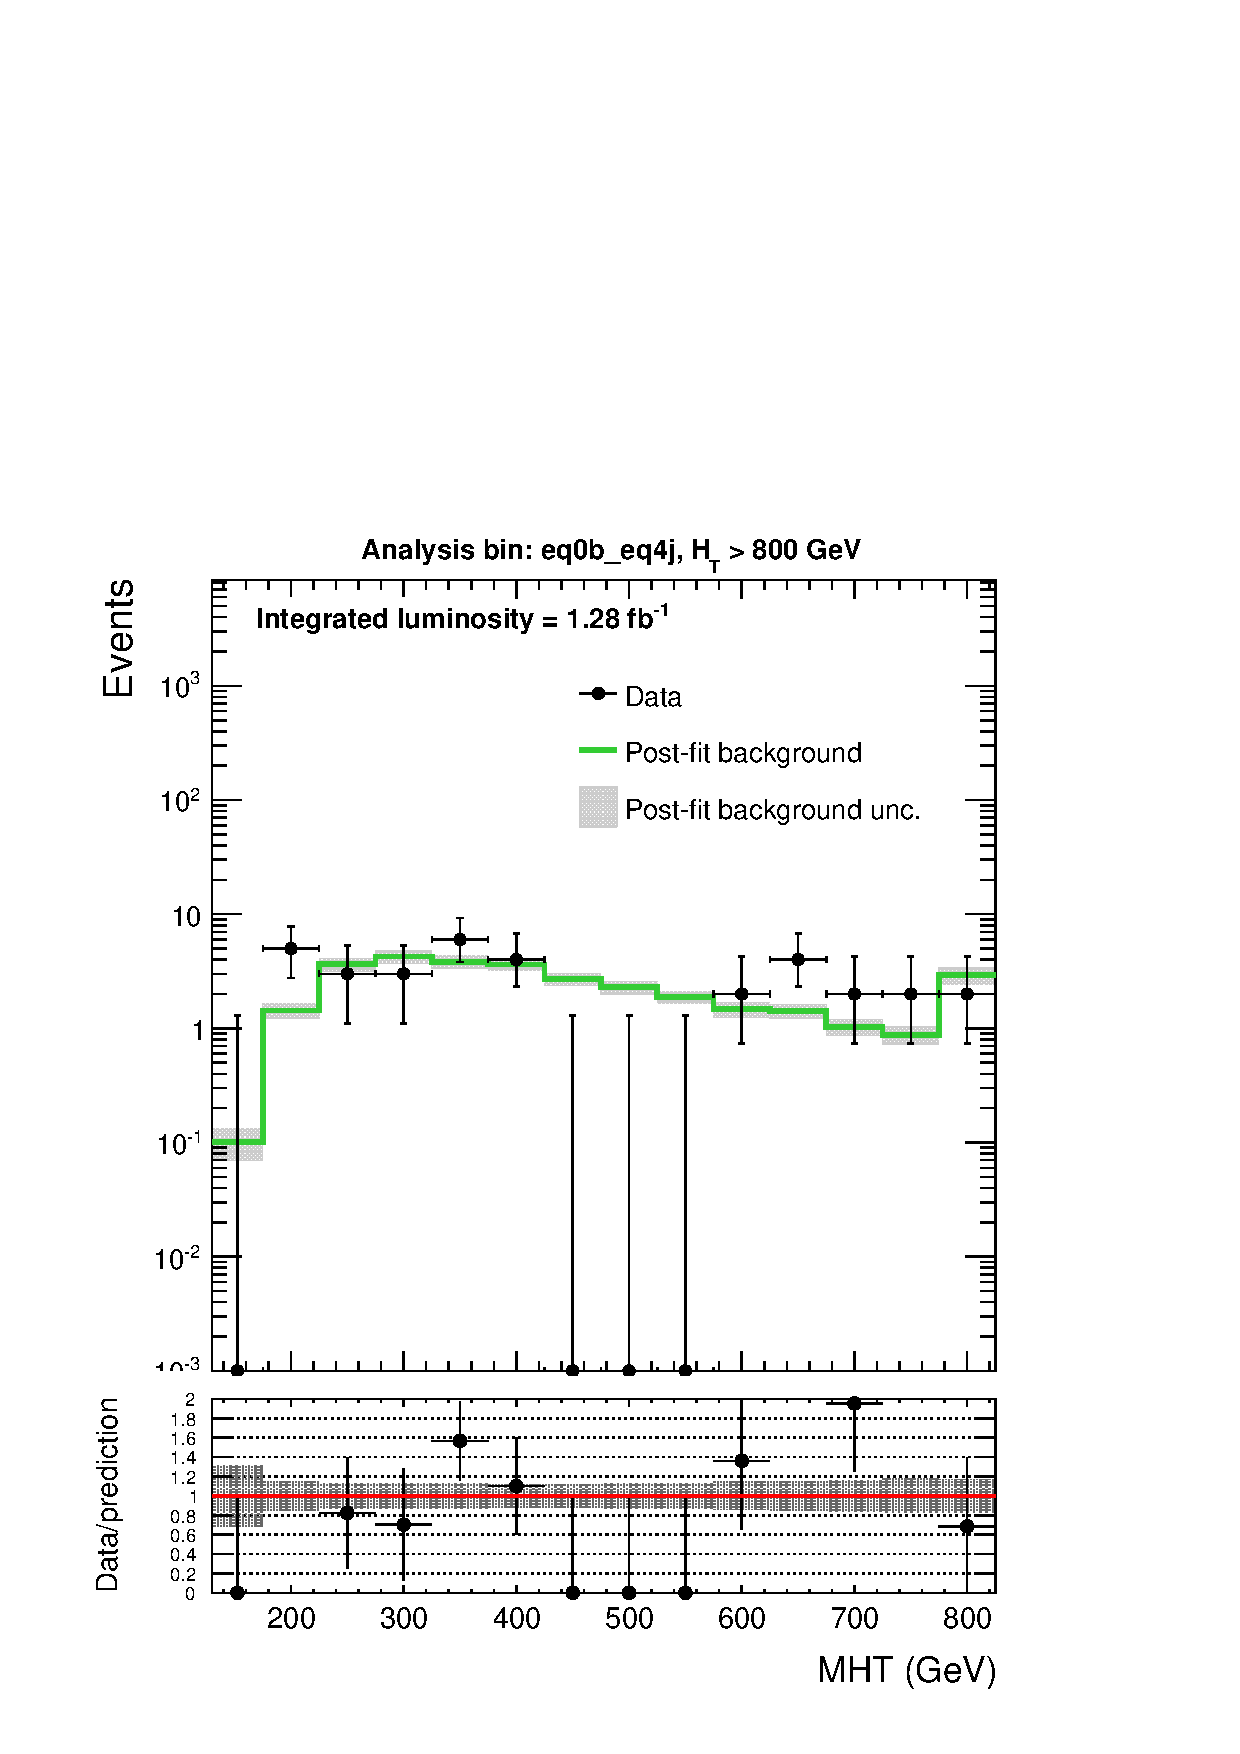
\includegraphics[width=0.25\textwidth]{figures/postFitResults/postFitShape_eq0b_eq4j_800_Inf.pdf} }\\
  \end{center}
\end{figure}



\newpage
\begin{figure}[h!]
\caption{Post-fit \MHT templates for the bin $\nj^{\mathrm{asym}}=5$, $\nb=0$ \label{fig:postFitShapes_eq0b_ge5a}}.
\begin{center}

    \subfigure[$\nj^{\mathrm{asym}}=5$, $\nb=0$, $300 < \scalht < 350 \; \mathrm{GeV}$]{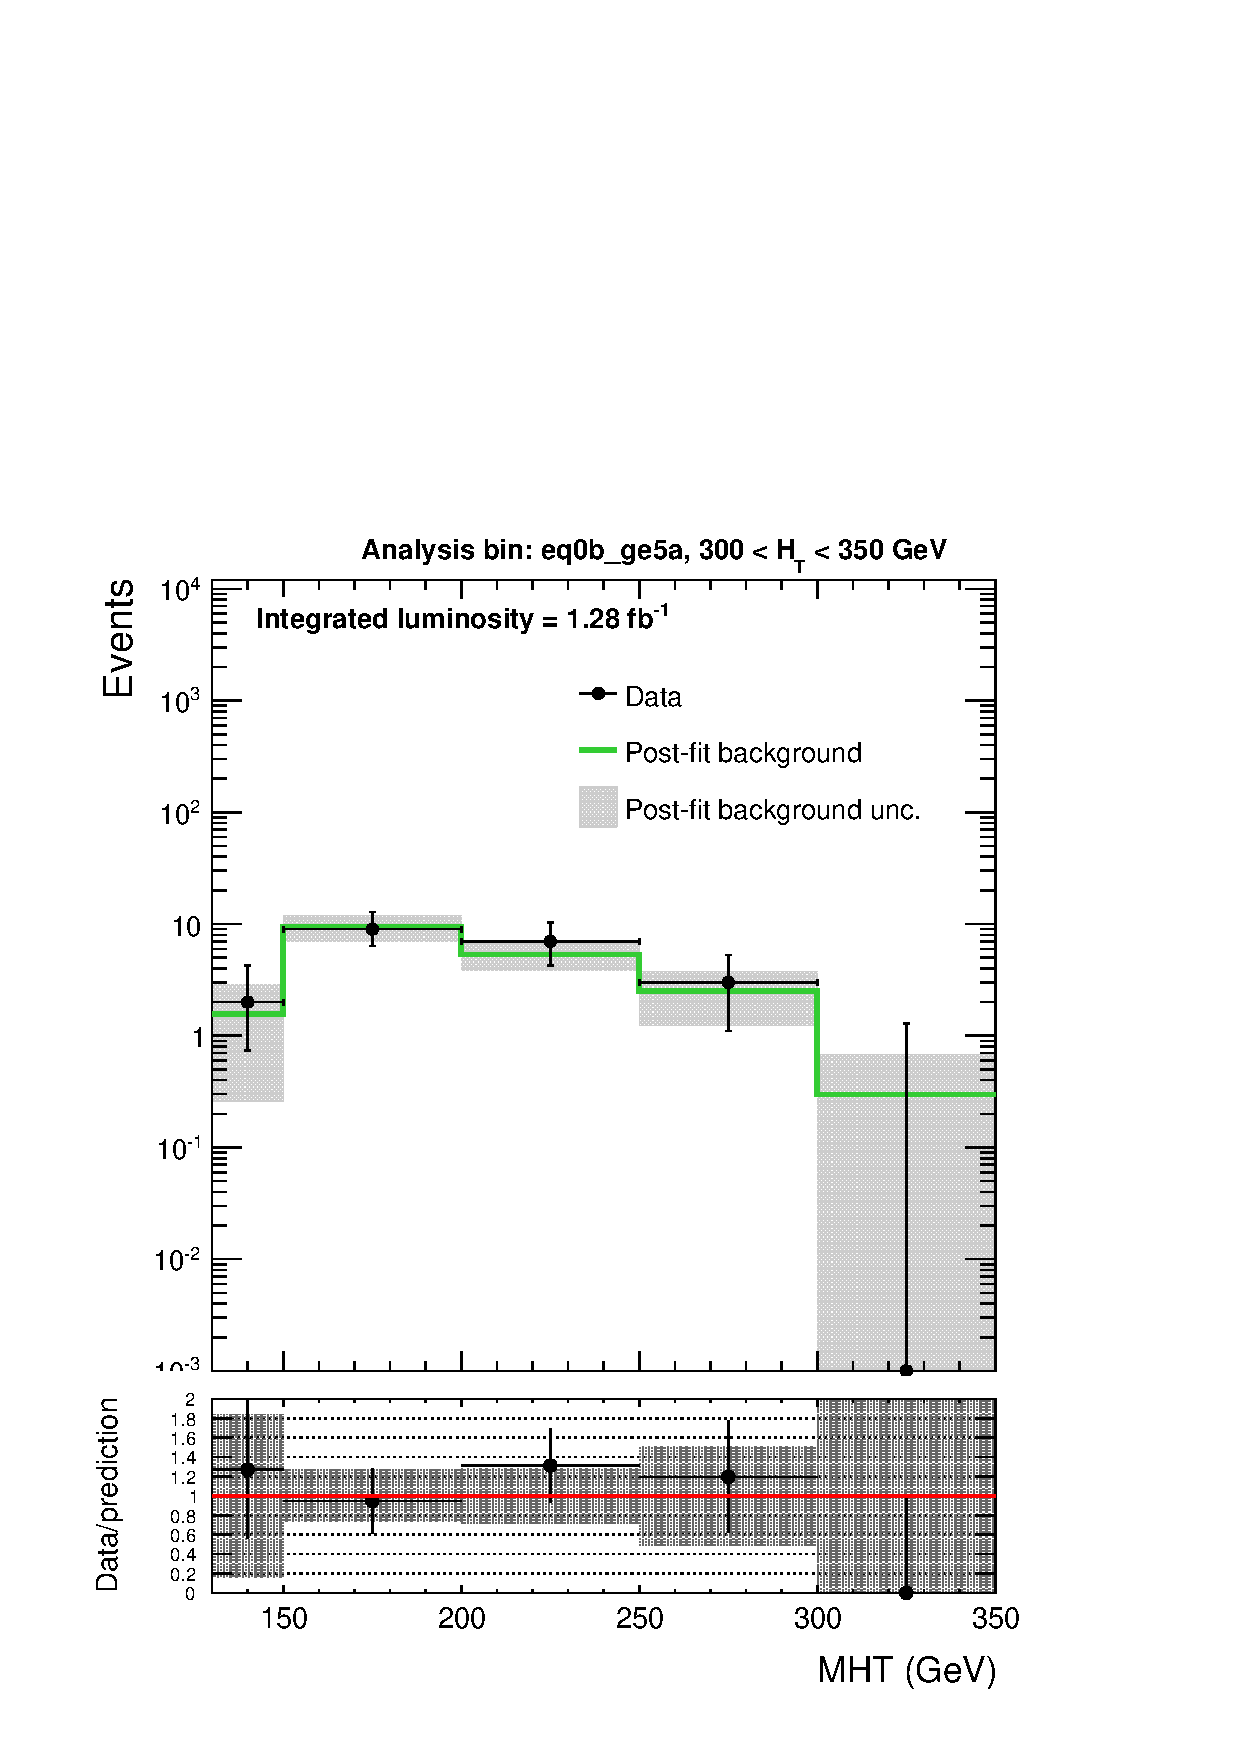
\includegraphics[width=0.25\textwidth]{figures/postFitResults/postFitShape_eq0b_ge5a_300_350.pdf} }\hspace{1cm}
    \subfigure[$\nj^{\mathrm{asym}}=5$, $\nb=0$, $350 < \scalht < 400 \; \mathrm{GeV}$]{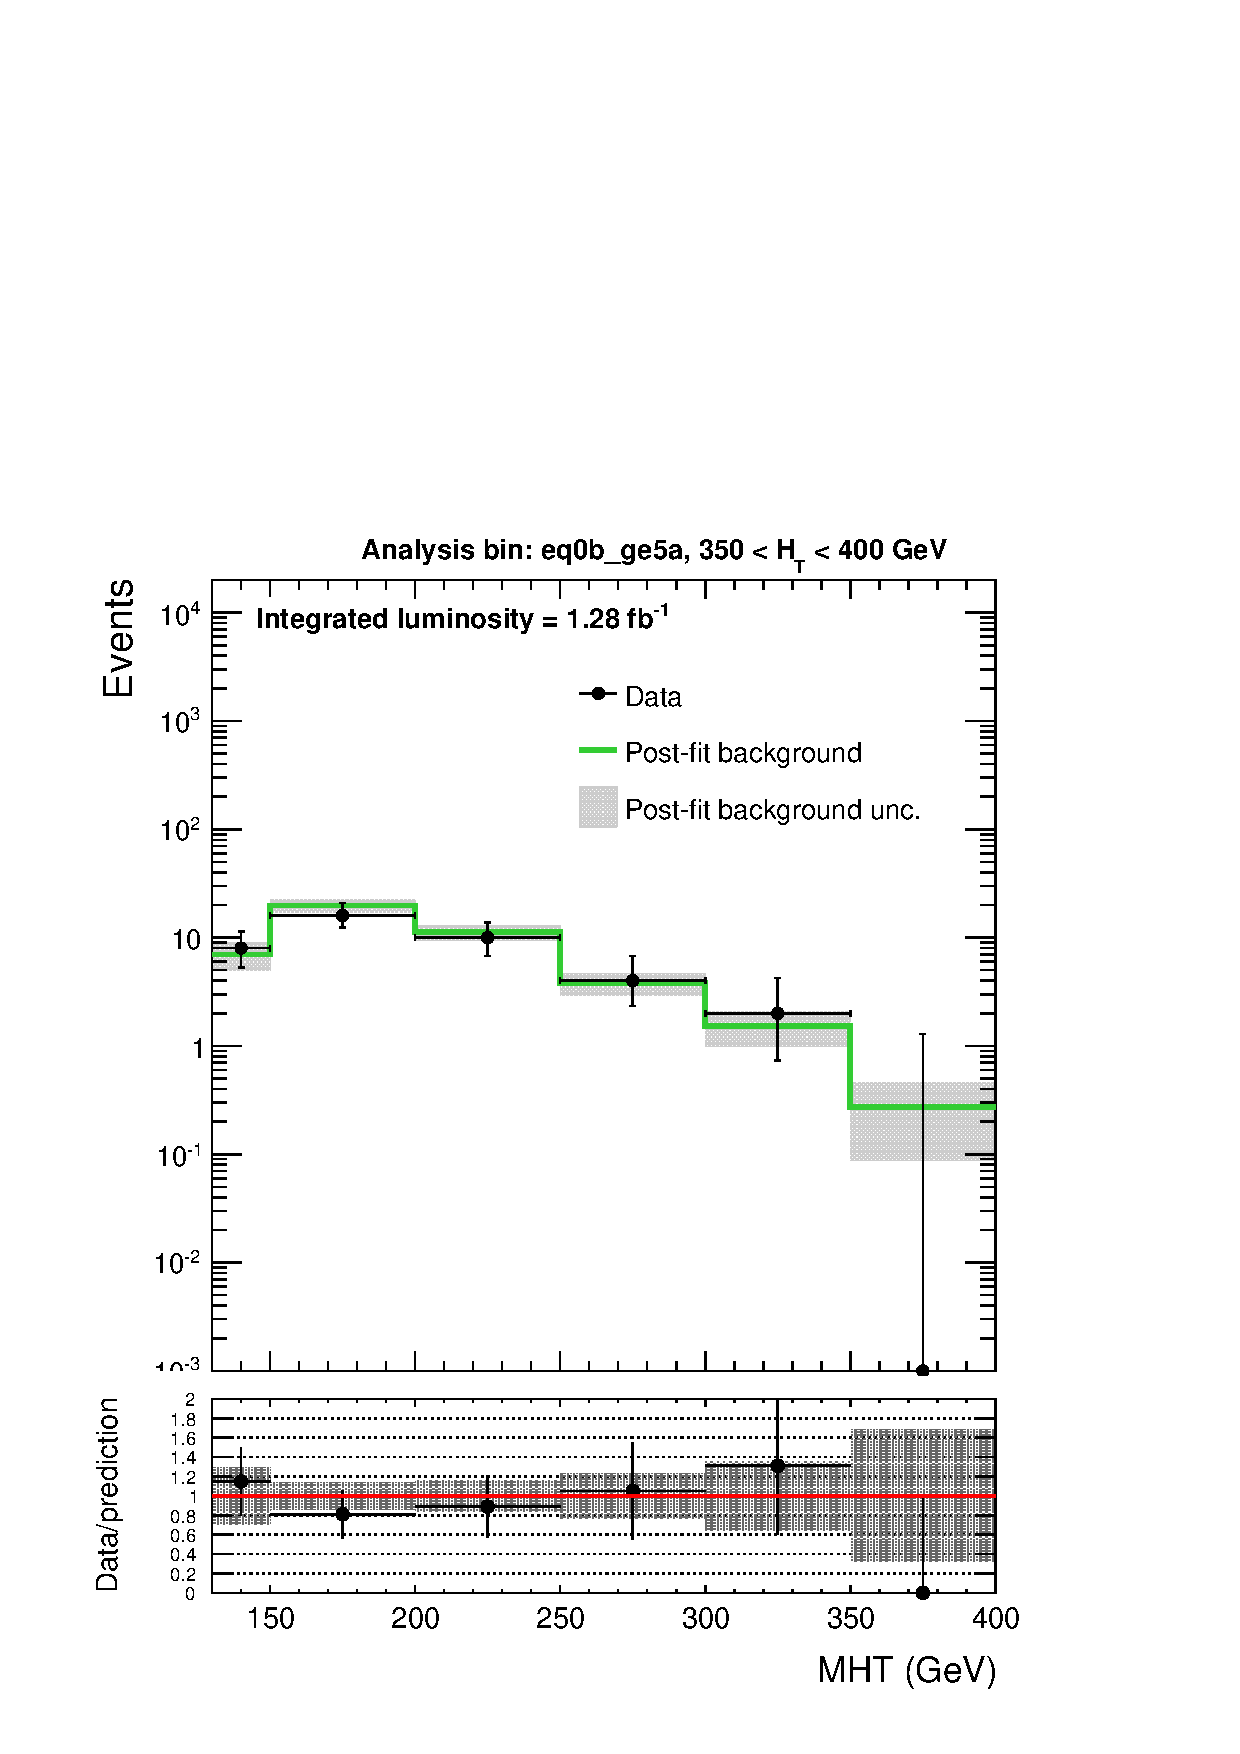
\includegraphics[width=0.25\textwidth]{figures/postFitResults/postFitShape_eq0b_ge5a_350_400.pdf} }\hspace{1cm}
    \subfigure[$\nj^{\mathrm{asym}}=5$, $\nb=0$, $400 < \scalht < 500 \; \mathrm{GeV}$]{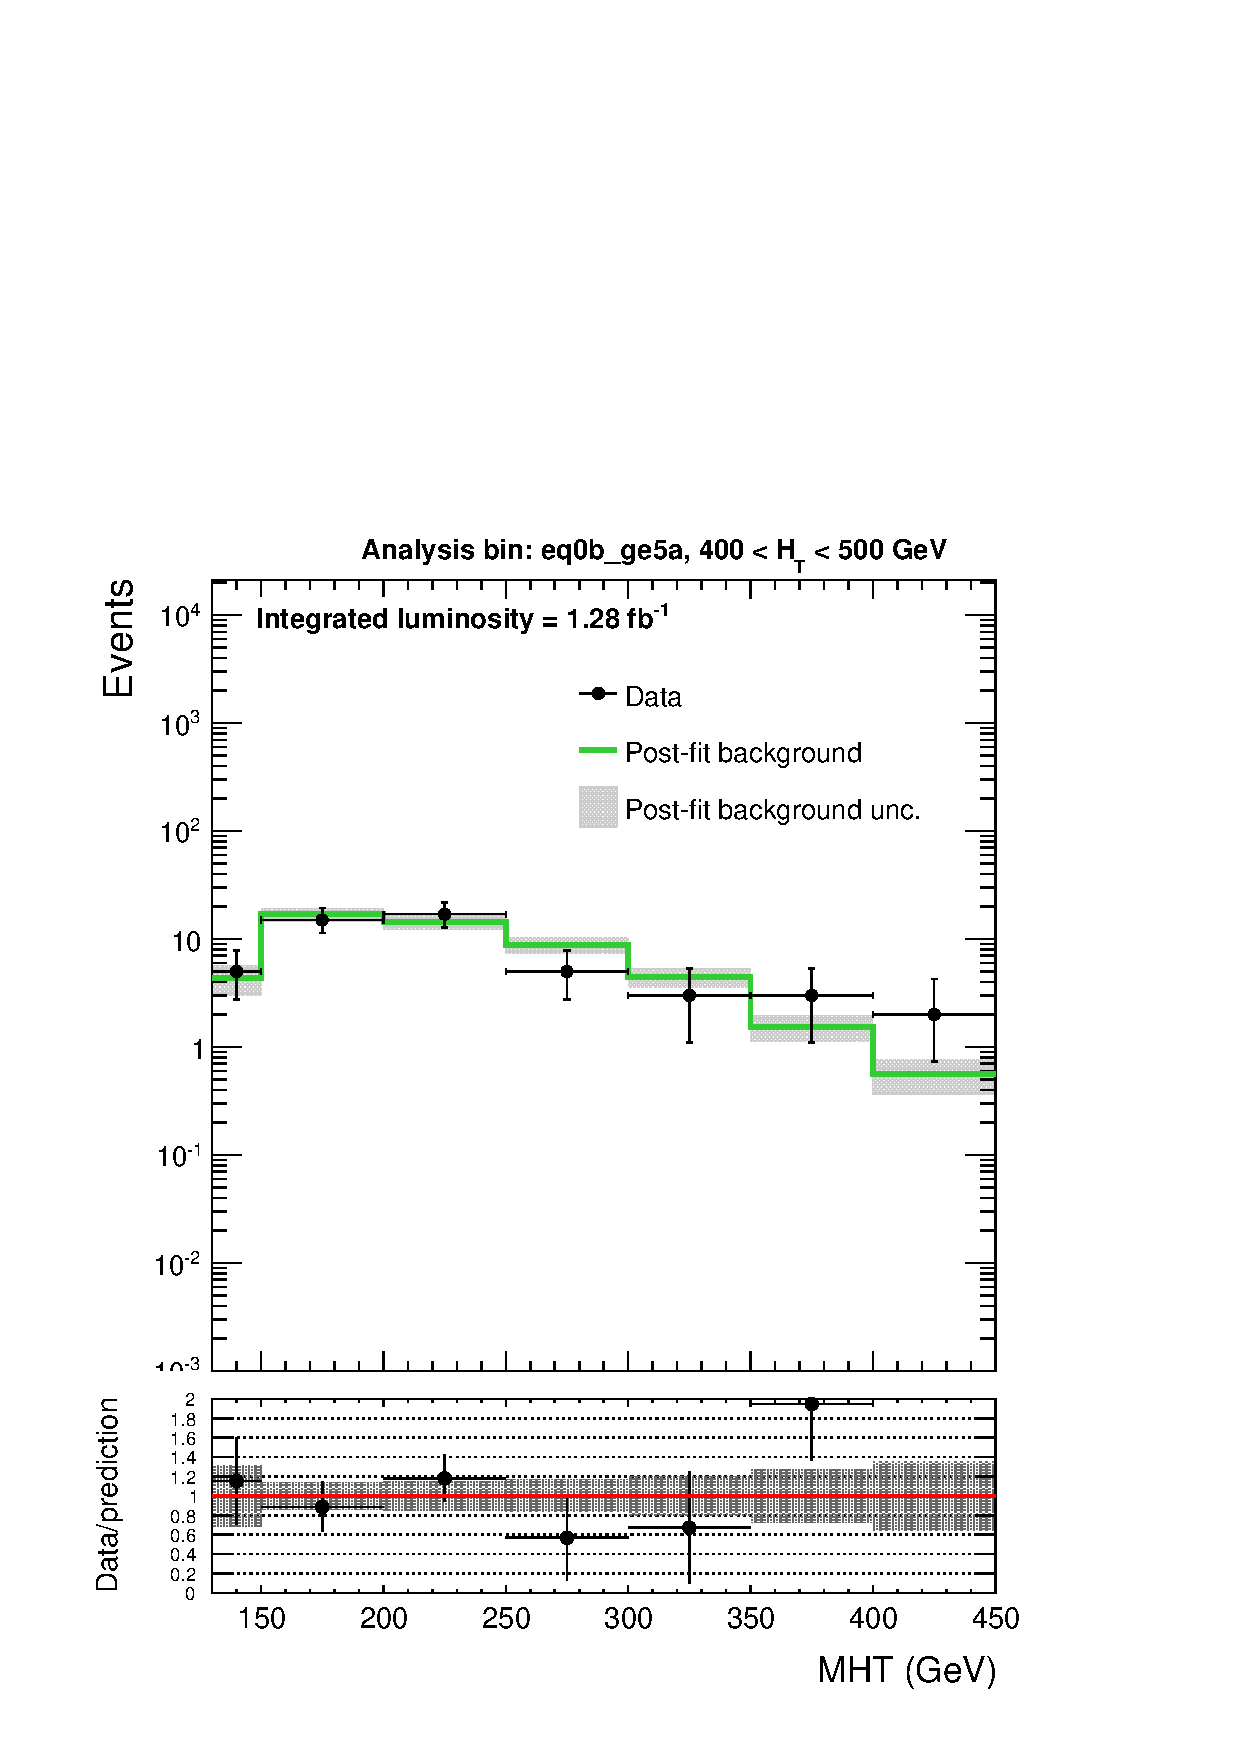
\includegraphics[width=0.25\textwidth]{figures/postFitResults/postFitShape_eq0b_ge5a_400_500.pdf} }\\
    \subfigure[$\nj^{\mathrm{asym}}=5$, $\nb=0$, $500 < \scalht < 600 \; \mathrm{GeV}$]{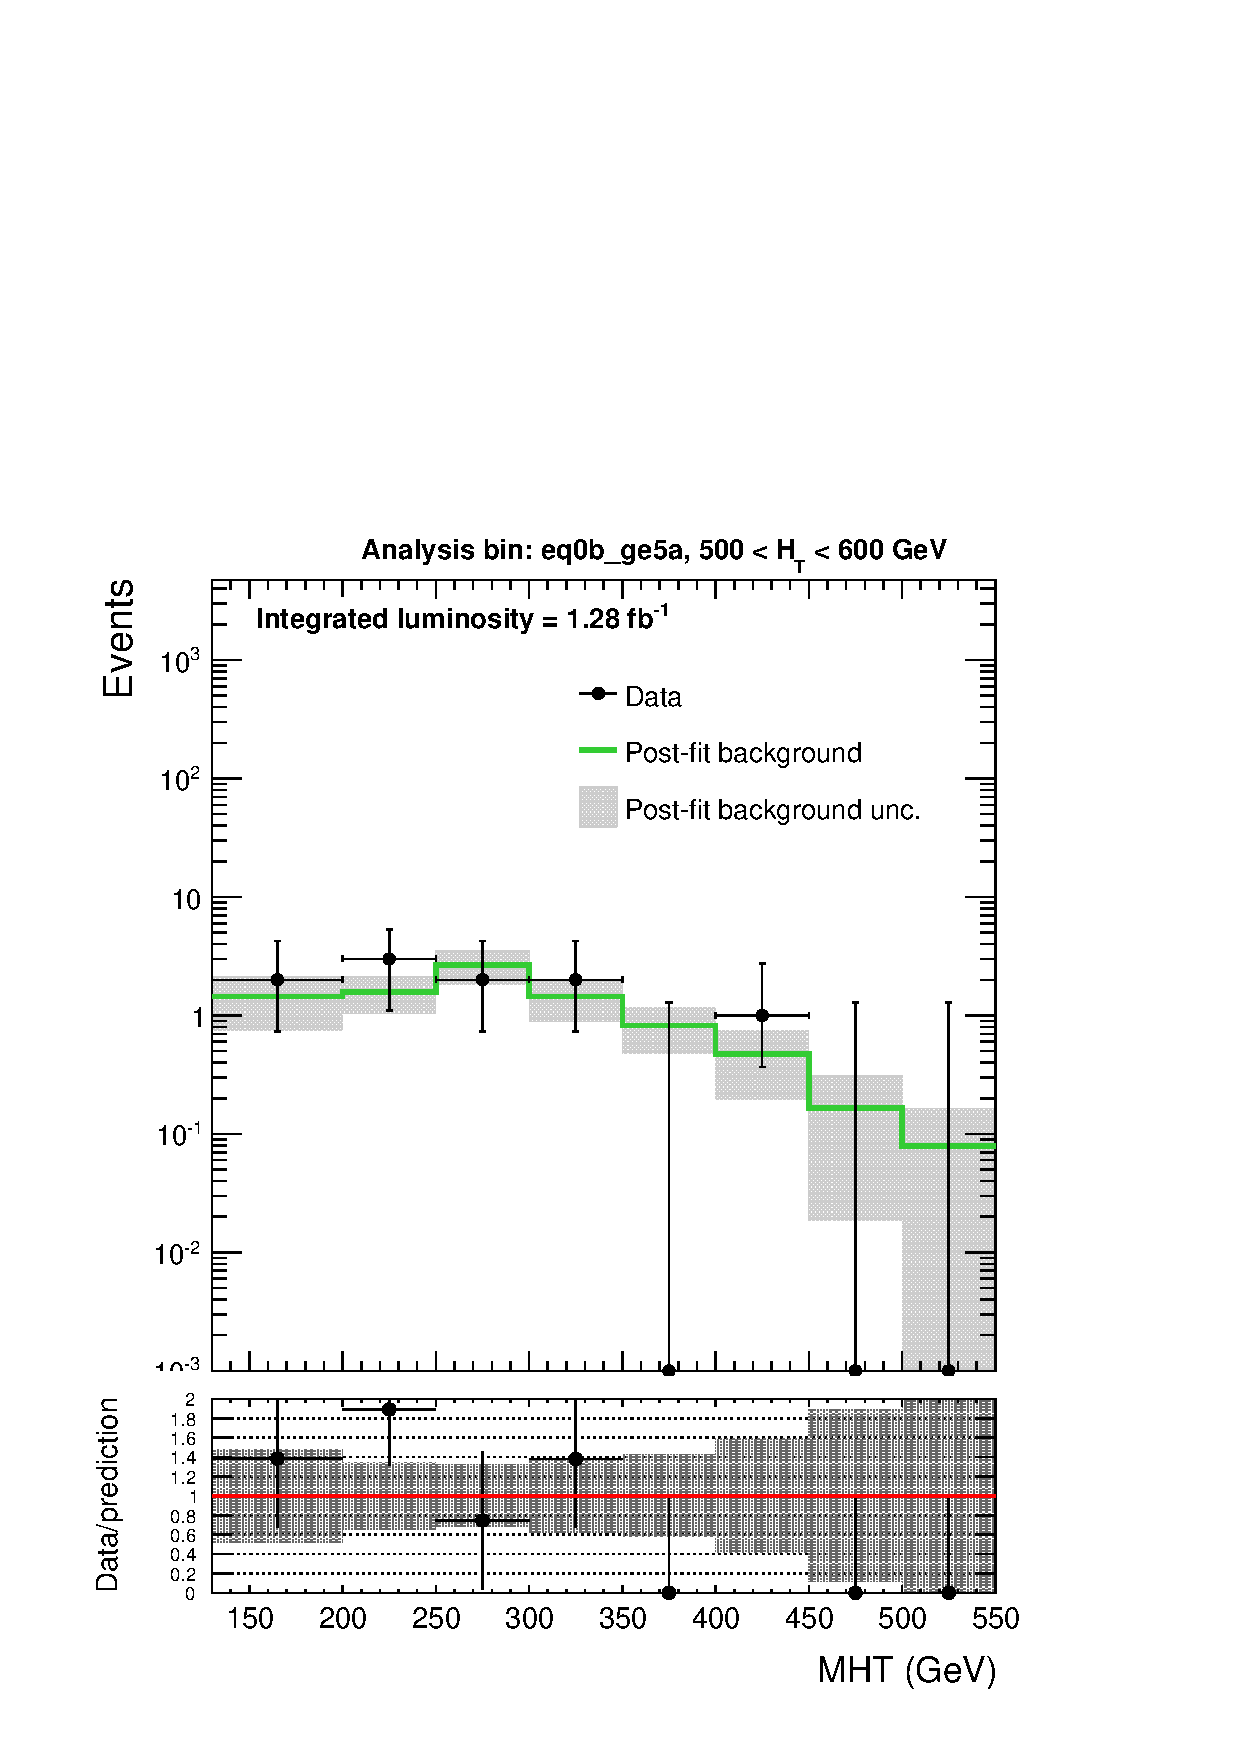
\includegraphics[width=0.25\textwidth]{figures/postFitResults/postFitShape_eq0b_ge5a_500_600.pdf} }\hspace{1cm}
  \end{center}
\end{figure}



\newpage
\begin{figure}[h!]
\caption{Post-fit \MHT templates for the bin $\nj^{\mathrm{sym}}=5$, $\nb=0$ \label{fig:postFitShapes_eq0b_ge5j}}.
\begin{center}

    \subfigure[$\nj^{\mathrm{sym}}=5$, $\nb=0$, $350 < \scalht < 400 \; \mathrm{GeV}$]{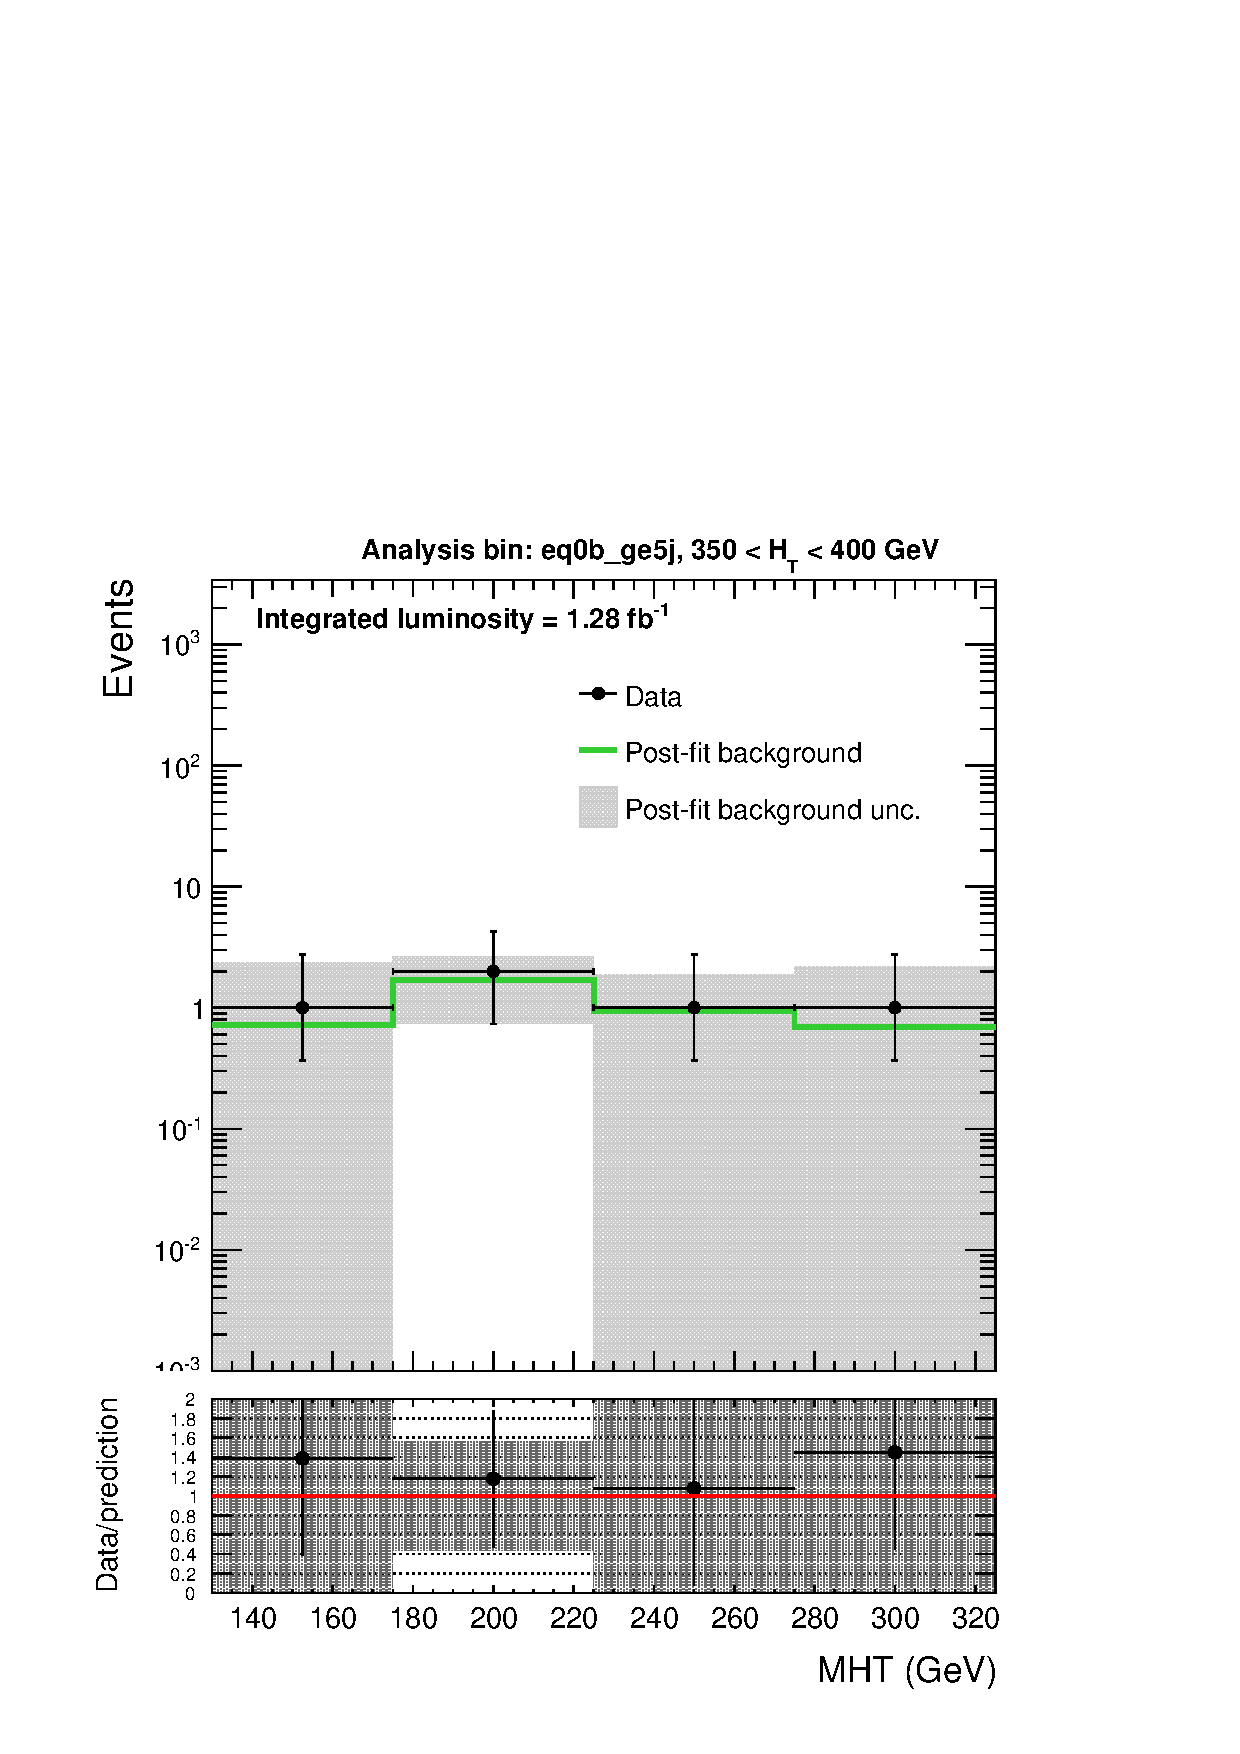
\includegraphics[width=0.25\textwidth]{figures/postFitResults/postFitShape_eq0b_ge5j_350_400.pdf} }\hspace{1cm}
    \subfigure[$\nj^{\mathrm{sym}}=5$, $\nb=0$, $400 < \scalht < 500 \; \mathrm{GeV}$]{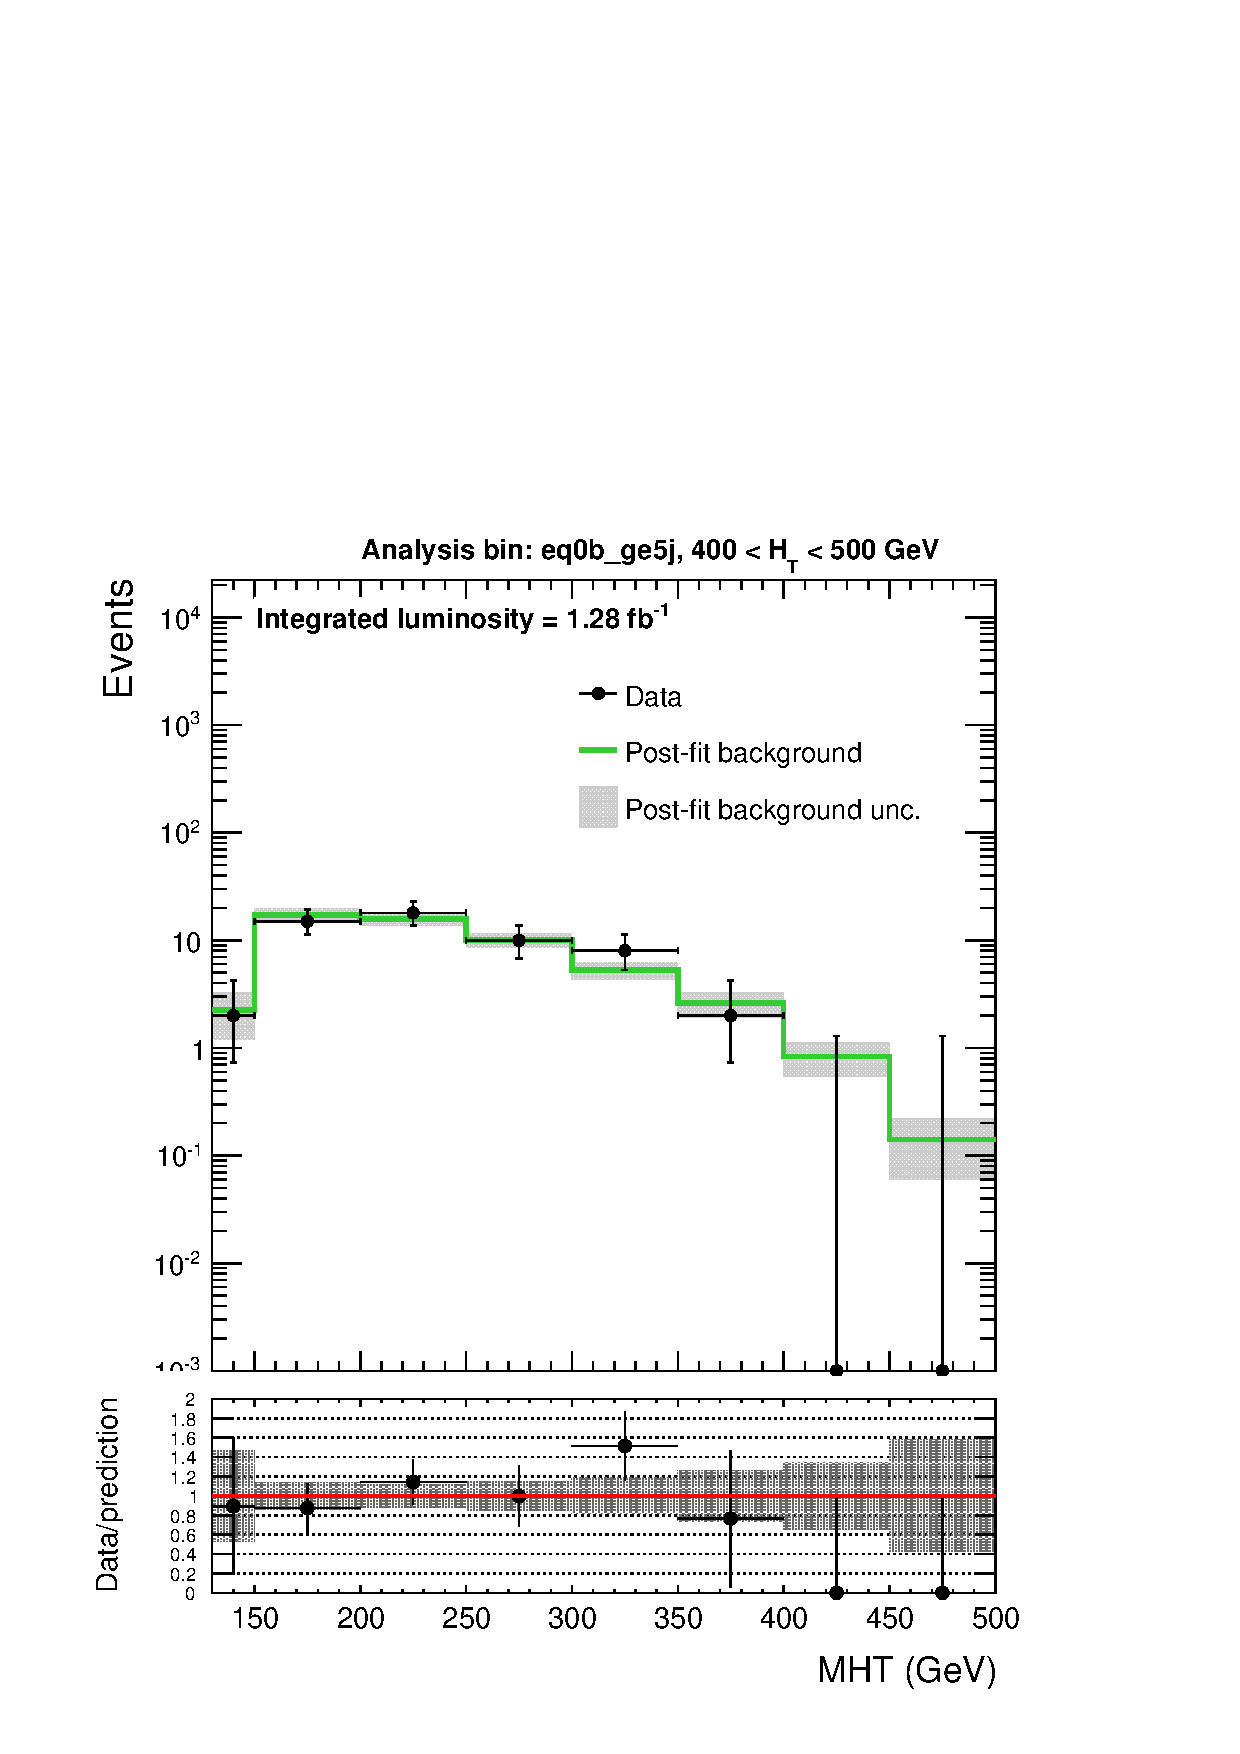
\includegraphics[width=0.25\textwidth]{figures/postFitResults/postFitShape_eq0b_ge5j_400_500.pdf} }\hspace{1cm}
    \subfigure[$\nj^{\mathrm{sym}}=5$, $\nb=0$, $500 < \scalht < 600 \; \mathrm{GeV}$]{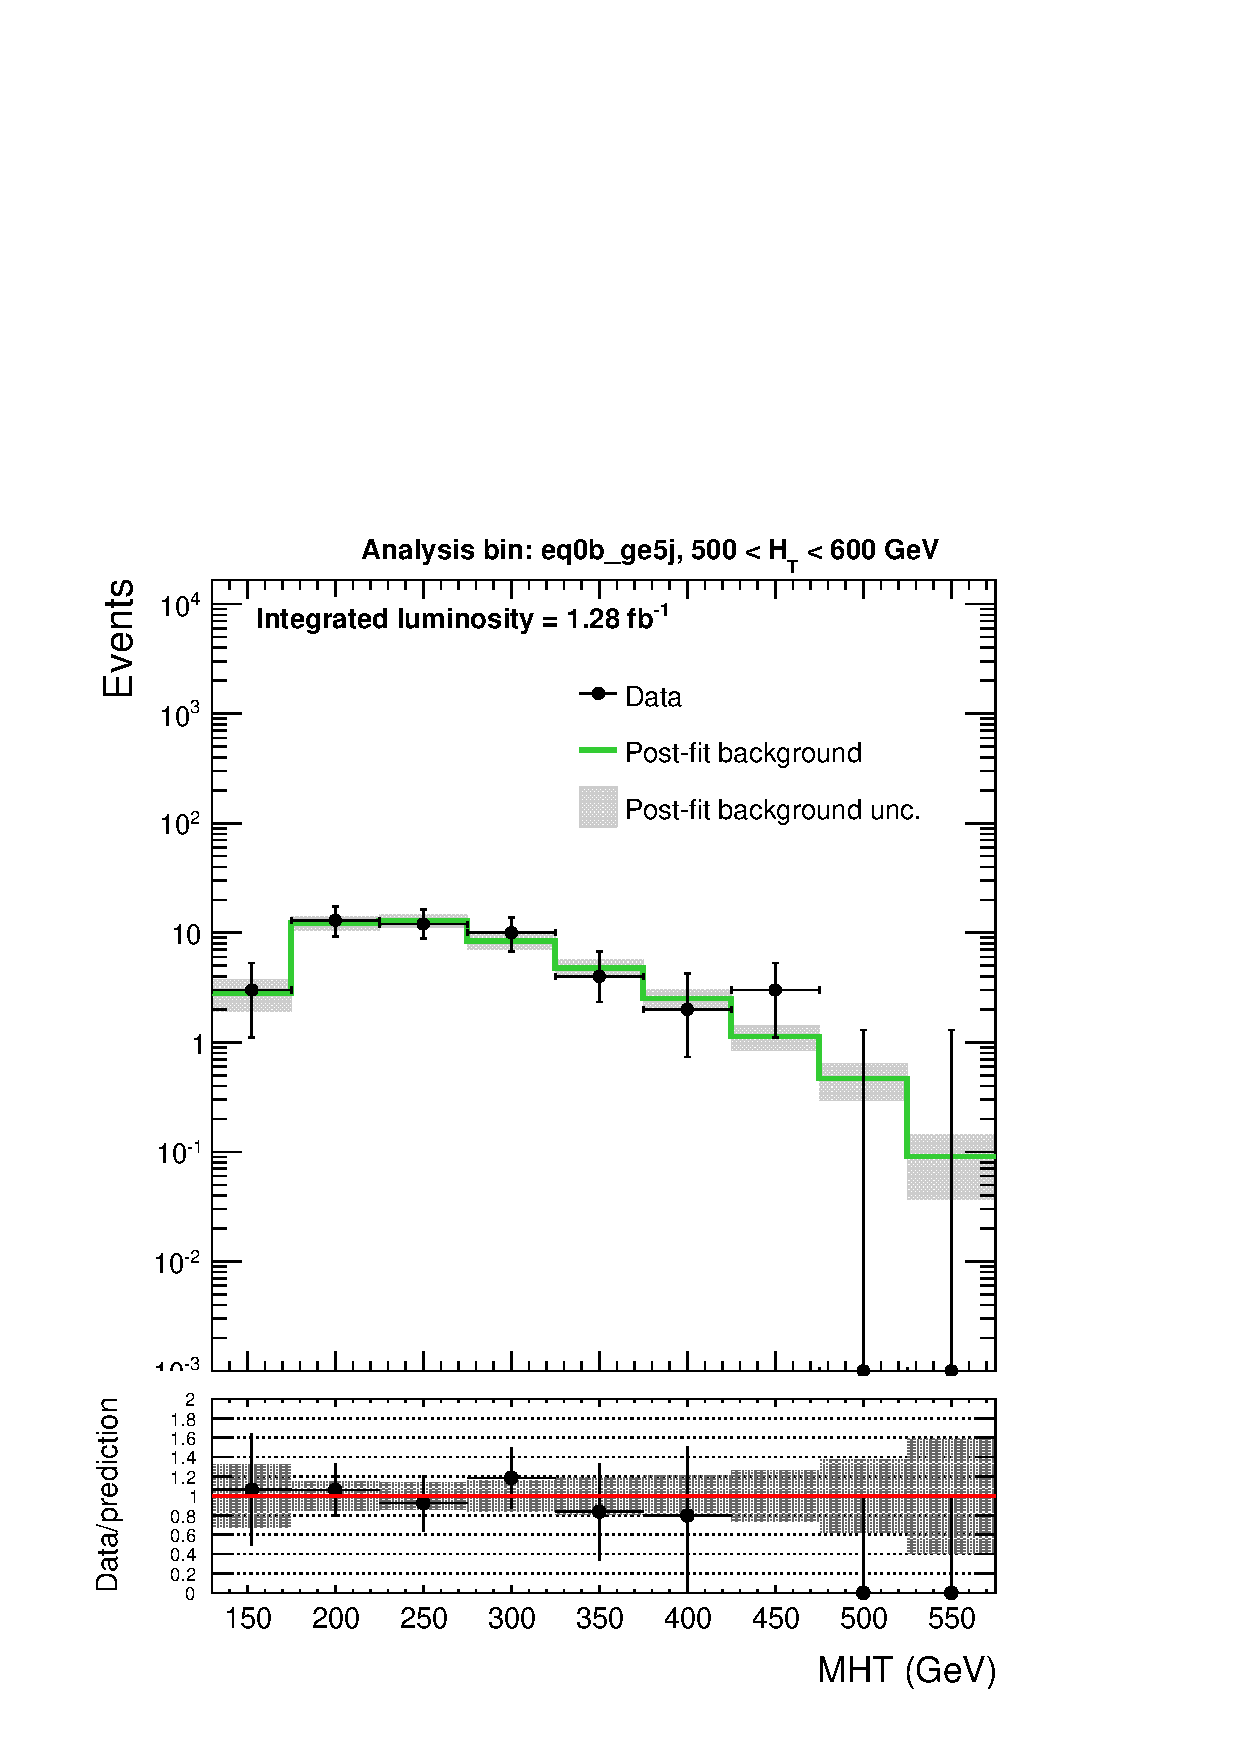
\includegraphics[width=0.25\textwidth]{figures/postFitResults/postFitShape_eq0b_ge5j_500_600.pdf} }\\
    \subfigure[$\nj^{\mathrm{sym}}=5$, $\nb=0$, $600 < \scalht < 800 \; \mathrm{GeV}$]{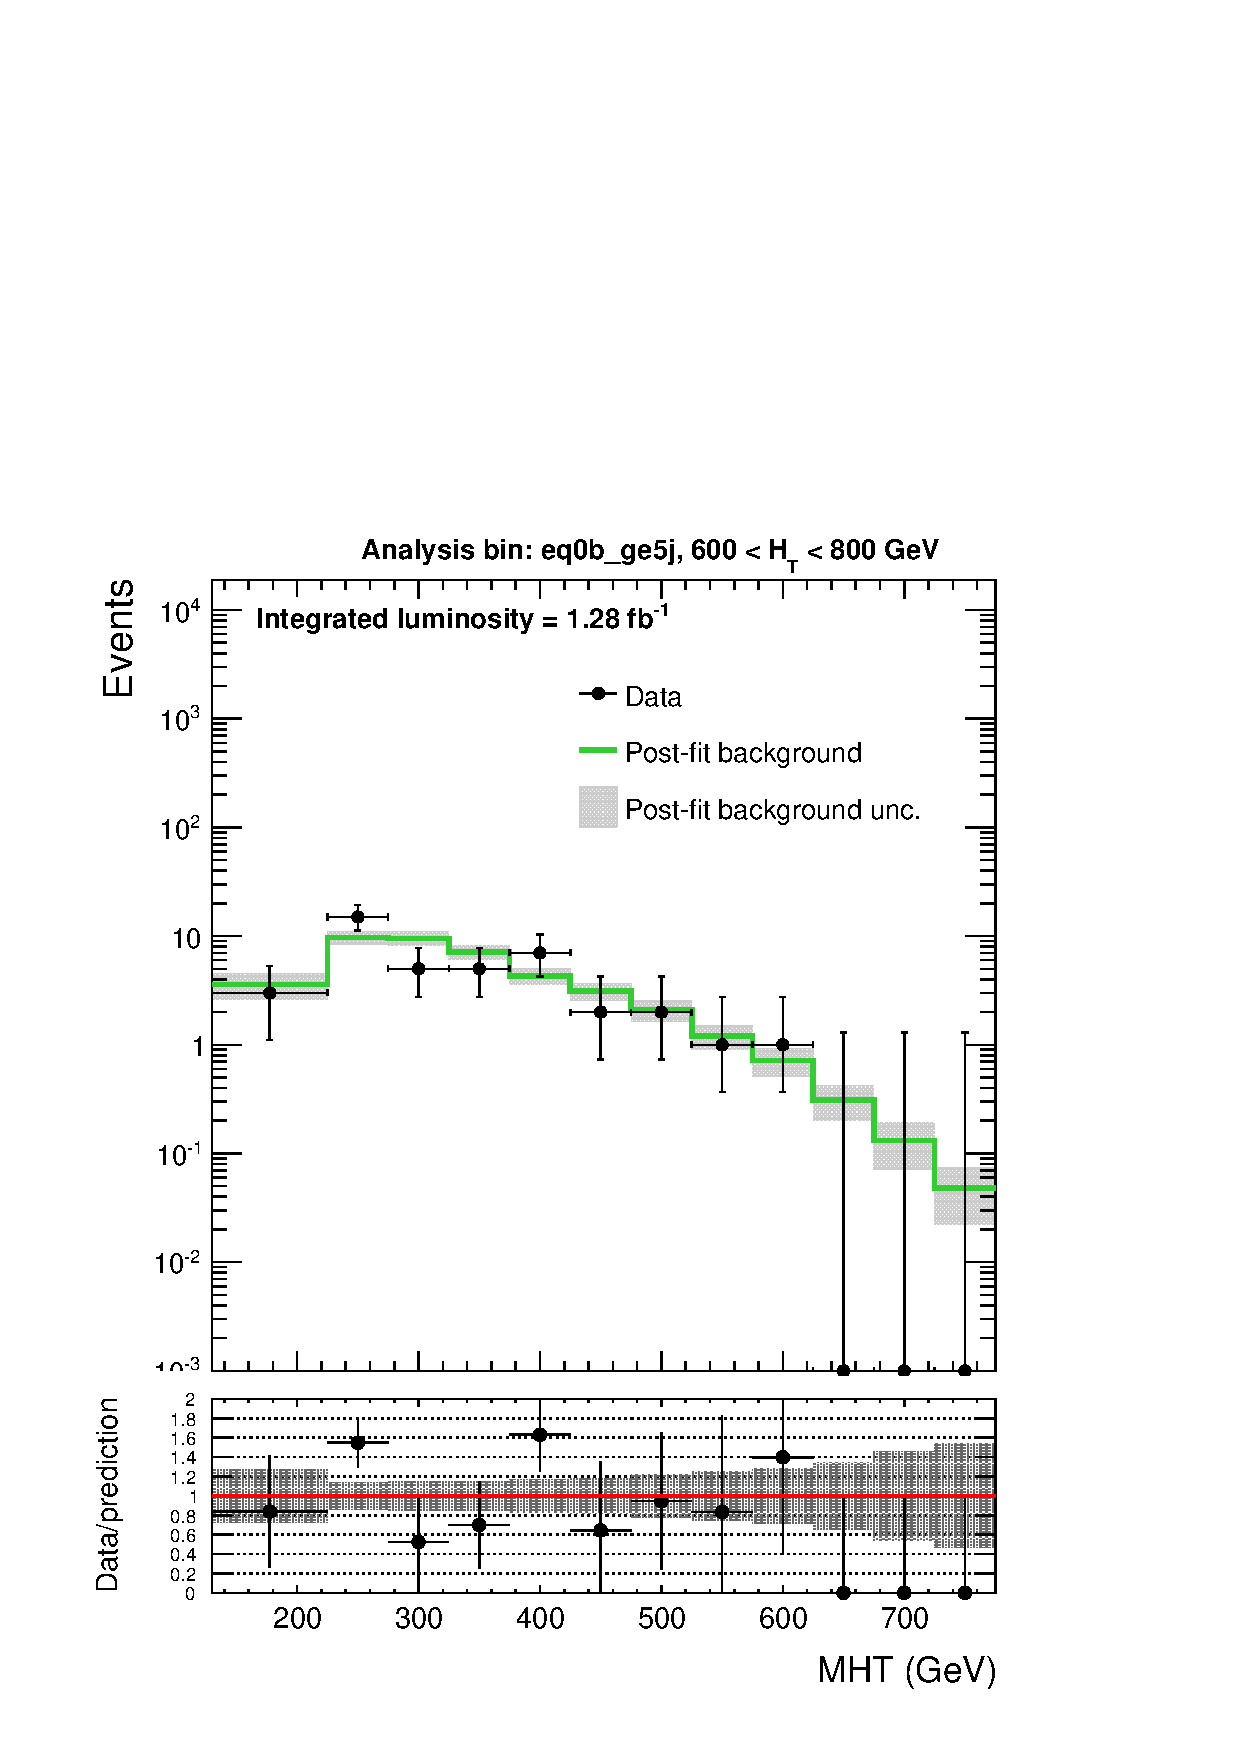
\includegraphics[width=0.25\textwidth]{figures/postFitResults/postFitShape_eq0b_ge5j_600_800.pdf} }\hspace{1cm}
    \subfigure[$\nj^{\mathrm{sym}}=5$, $\nb=0$, $\scalht > 800 \; \mathrm{GeV}$]{\includegraphics[width=0.25\textwidth]{figures/postFitResults/postFitShape_eq0b_ge5j_800_Inf.pdf} }\hspace{1cm}
  \end{center}
\end{figure}



\newpage
\begin{figure}[h!]
\caption{Post-fit \MHT templates for the bin $\nj^{\mathrm{asym}}=2$, $\nb=1$ \label{fig:postFitShapes_eq1b_eq2a}}.
\begin{center}

    \subfigure[$\nj^{\mathrm{asym}}=2$, $\nb=1$, $200 < \scalht < 250 \; \mathrm{GeV}$]{\includegraphics[width=0.25\textwidth]{figures/postFitResults/postFitShape_eq1b_eq2a_200_250.pdf} }\hspace{1cm}
    \subfigure[$\nj^{\mathrm{asym}}=2$, $\nb=1$, $250 < \scalht < 300 \; \mathrm{GeV}$]{\includegraphics[width=0.25\textwidth]{figures/postFitResults/postFitShape_eq1b_eq2a_250_300.pdf} }\hspace{1cm}
    \subfigure[$\nj^{\mathrm{asym}}=2$, $\nb=1$, $300 < \scalht < 350 \; \mathrm{GeV}$]{\includegraphics[width=0.25\textwidth]{figures/postFitResults/postFitShape_eq1b_eq2a_300_350.pdf} }\\
    \subfigure[$\nj^{\mathrm{asym}}=2$, $\nb=1$, $350 < \scalht < 400 \; \mathrm{GeV}$]{\includegraphics[width=0.25\textwidth]{figures/postFitResults/postFitShape_eq1b_eq2a_350_400.pdf} }\hspace{1cm}
    \subfigure[$\nj^{\mathrm{asym}}=2$, $\nb=1$, $400 < \scalht < 500 \; \mathrm{GeV}$]{\includegraphics[width=0.25\textwidth]{figures/postFitResults/postFitShape_eq1b_eq2a_400_500.pdf} }\hspace{1cm}
    \subfigure[$\nj^{\mathrm{asym}}=2$, $\nb=1$, $500 < \scalht < 600 \; \mathrm{GeV}$]{\includegraphics[width=0.25\textwidth]{figures/postFitResults/postFitShape_eq1b_eq2a_500_600.pdf} }\\
  \end{center}
\end{figure}



\newpage
\begin{figure}[h!]
\caption{Post-fit \MHT templates for the bin $\nj^{\mathrm{sym}}=2$, $\nb=1$ \label{fig:postFitShapes_eq1b_eq2j}}.
\begin{center}

    \subfigure[$\nj^{\mathrm{sym}}=2$, $\nb=1$, $200 < \scalht < 250 \; \mathrm{GeV}$]{\includegraphics[width=0.25\textwidth]{figures/postFitResults/postFitShape_eq1b_eq2j_200_250.pdf} }\hspace{1cm}
    \subfigure[$\nj^{\mathrm{sym}}=2$, $\nb=1$, $250 < \scalht < 300 \; \mathrm{GeV}$]{\includegraphics[width=0.25\textwidth]{figures/postFitResults/postFitShape_eq1b_eq2j_250_300.pdf} }\hspace{1cm}
    \subfigure[$\nj^{\mathrm{sym}}=2$, $\nb=1$, $300 < \scalht < 350 \; \mathrm{GeV}$]{\includegraphics[width=0.25\textwidth]{figures/postFitResults/postFitShape_eq1b_eq2j_300_350.pdf} }\\
    \subfigure[$\nj^{\mathrm{sym}}=2$, $\nb=1$, $350 < \scalht < 400 \; \mathrm{GeV}$]{\includegraphics[width=0.25\textwidth]{figures/postFitResults/postFitShape_eq1b_eq2j_350_400.pdf} }\hspace{1cm}
    \subfigure[$\nj^{\mathrm{sym}}=2$, $\nb=1$, $400 < \scalht < 500 \; \mathrm{GeV}$]{\includegraphics[width=0.25\textwidth]{figures/postFitResults/postFitShape_eq1b_eq2j_400_500.pdf} }\hspace{1cm}
    \subfigure[$\nj^{\mathrm{sym}}=2$, $\nb=1$, $500 < \scalht < 600 \; \mathrm{GeV}$]{\includegraphics[width=0.25\textwidth]{figures/postFitResults/postFitShape_eq1b_eq2j_500_600.pdf} }\\
    \subfigure[$\nj^{\mathrm{sym}}=2$, $\nb=1$, $600 < \scalht < 800 \; \mathrm{GeV}$]{\includegraphics[width=0.25\textwidth]{figures/postFitResults/postFitShape_eq1b_eq2j_600_800.pdf} }\hspace{1cm}
    \subfigure[$\nj^{\mathrm{sym}}=2$, $\nb=1$, $\scalht > 800 \; \mathrm{GeV}$]{\includegraphics[width=0.25\textwidth]{figures/postFitResults/postFitShape_eq1b_eq2j_800_Inf.pdf} }\hspace{1cm}
  \end{center}
\end{figure}



\newpage
\begin{figure}[h!]
\caption{Post-fit \MHT templates for the bin $\nj^{\mathrm{asym}}=3$, $\nb=1$ \label{fig:postFitShapes_eq1b_eq3a}}.
\begin{center}

    \subfigure[$\nj^{\mathrm{asym}}=3$, $\nb=1$, $200 < \scalht < 250 \; \mathrm{GeV}$]{\includegraphics[width=0.25\textwidth]{figures/postFitResults/postFitShape_eq1b_eq3a_200_250.pdf} }\hspace{1cm}
    \subfigure[$\nj^{\mathrm{asym}}=3$, $\nb=1$, $250 < \scalht < 300 \; \mathrm{GeV}$]{\includegraphics[width=0.25\textwidth]{figures/postFitResults/postFitShape_eq1b_eq3a_250_300.pdf} }\hspace{1cm}
    \subfigure[$\nj^{\mathrm{asym}}=3$, $\nb=1$, $300 < \scalht < 350 \; \mathrm{GeV}$]{\includegraphics[width=0.25\textwidth]{figures/postFitResults/postFitShape_eq1b_eq3a_300_350.pdf} }\\
    \subfigure[$\nj^{\mathrm{asym}}=3$, $\nb=1$, $350 < \scalht < 400 \; \mathrm{GeV}$]{\includegraphics[width=0.25\textwidth]{figures/postFitResults/postFitShape_eq1b_eq3a_350_400.pdf} }\hspace{1cm}
    \subfigure[$\nj^{\mathrm{asym}}=3$, $\nb=1$, $400 < \scalht < 500 \; \mathrm{GeV}$]{\includegraphics[width=0.25\textwidth]{figures/postFitResults/postFitShape_eq1b_eq3a_400_500.pdf} }\hspace{1cm}
    \subfigure[$\nj^{\mathrm{asym}}=3$, $\nb=1$, $500 < \scalht < 600 \; \mathrm{GeV}$]{\includegraphics[width=0.25\textwidth]{figures/postFitResults/postFitShape_eq1b_eq3a_500_600.pdf} }\\
    \subfigure[$\nj^{\mathrm{asym}}=3$, $\nb=1$, $\scalht > 600 \; \mathrm{GeV}$]{\includegraphics[width=0.25\textwidth]{figures/postFitResults/postFitShape_eq1b_eq3a_600_Inf.pdf} }\hspace{1cm}
  \end{center}
\end{figure}



\newpage
\begin{figure}[h!]
\caption{Post-fit \MHT templates for the bin $\nj^{\mathrm{sym}}=3$, $\nb=1$ \label{fig:postFitShapes_eq1b_eq3j}}.
\begin{center}

    \subfigure[$\nj^{\mathrm{sym}}=3$, $\nb=1$, $250 < \scalht < 300 \; \mathrm{GeV}$]{\includegraphics[width=0.25\textwidth]{figures/postFitResults/postFitShape_eq1b_eq3j_250_300.pdf} }\hspace{1cm}
    \subfigure[$\nj^{\mathrm{sym}}=3$, $\nb=1$, $300 < \scalht < 350 \; \mathrm{GeV}$]{\includegraphics[width=0.25\textwidth]{figures/postFitResults/postFitShape_eq1b_eq3j_300_350.pdf} }\hspace{1cm}
    \subfigure[$\nj^{\mathrm{sym}}=3$, $\nb=1$, $350 < \scalht < 400 \; \mathrm{GeV}$]{\includegraphics[width=0.25\textwidth]{figures/postFitResults/postFitShape_eq1b_eq3j_350_400.pdf} }\\
    \subfigure[$\nj^{\mathrm{sym}}=3$, $\nb=1$, $400 < \scalht < 500 \; \mathrm{GeV}$]{\includegraphics[width=0.25\textwidth]{figures/postFitResults/postFitShape_eq1b_eq3j_400_500.pdf} }\hspace{1cm}
    \subfigure[$\nj^{\mathrm{sym}}=3$, $\nb=1$, $500 < \scalht < 600 \; \mathrm{GeV}$]{\includegraphics[width=0.25\textwidth]{figures/postFitResults/postFitShape_eq1b_eq3j_500_600.pdf} }\hspace{1cm}
    \subfigure[$\nj^{\mathrm{sym}}=3$, $\nb=1$, $600 < \scalht < 800 \; \mathrm{GeV}$]{\includegraphics[width=0.25\textwidth]{figures/postFitResults/postFitShape_eq1b_eq3j_600_800.pdf} }\\
    \subfigure[$\nj^{\mathrm{sym}}=3$, $\nb=1$, $\scalht > 800 \; \mathrm{GeV}$]{\includegraphics[width=0.25\textwidth]{figures/postFitResults/postFitShape_eq1b_eq3j_800_Inf.pdf} }\hspace{1cm}
  \end{center}
\end{figure}



\newpage
\begin{figure}[h!]
\caption{Post-fit \MHT templates for the bin $\nj^{\mathrm{asym}}=4$, $\nb=1$ \label{fig:postFitShapes_eq1b_eq4a}}.
\begin{center}

    \subfigure[$\nj^{\mathrm{asym}}=4$, $\nb=1$, $250 < \scalht < 300 \; \mathrm{GeV}$]{\includegraphics[width=0.25\textwidth]{figures/postFitResults/postFitShape_eq1b_eq4a_250_300.pdf} }\hspace{1cm}
    \subfigure[$\nj^{\mathrm{asym}}=4$, $\nb=1$, $300 < \scalht < 350 \; \mathrm{GeV}$]{\includegraphics[width=0.25\textwidth]{figures/postFitResults/postFitShape_eq1b_eq4a_300_350.pdf} }\hspace{1cm}
    \subfigure[$\nj^{\mathrm{asym}}=4$, $\nb=1$, $350 < \scalht < 400 \; \mathrm{GeV}$]{\includegraphics[width=0.25\textwidth]{figures/postFitResults/postFitShape_eq1b_eq4a_350_400.pdf} }\\
    \subfigure[$\nj^{\mathrm{asym}}=4$, $\nb=1$, $400 < \scalht < 500 \; \mathrm{GeV}$]{\includegraphics[width=0.25\textwidth]{figures/postFitResults/postFitShape_eq1b_eq4a_400_500.pdf} }\hspace{1cm}
    \subfigure[$\nj^{\mathrm{asym}}=4$, $\nb=1$, $500 < \scalht < 600 \; \mathrm{GeV}$]{\includegraphics[width=0.25\textwidth]{figures/postFitResults/postFitShape_eq1b_eq4a_500_600.pdf} }\hspace{1cm}
    \subfigure[$\nj^{\mathrm{asym}}=4$, $\nb=1$, $\scalht > 600 \; \mathrm{GeV}$]{\includegraphics[width=0.25\textwidth]{figures/postFitResults/postFitShape_eq1b_eq4a_600_Inf.pdf} }\\
  \end{center}
\end{figure}



\newpage
\begin{figure}[h!]
\caption{Post-fit \MHT templates for the bin $\nj^{\mathrm{sym}}=4$, $\nb=1$ \label{fig:postFitShapes_eq1b_eq4j}}.
\begin{center}

    \subfigure[$\nj^{\mathrm{sym}}=4$, $\nb=1$, $300 < \scalht < 350 \; \mathrm{GeV}$]{\includegraphics[width=0.25\textwidth]{figures/postFitResults/postFitShape_eq1b_eq4j_300_350.pdf} }\hspace{1cm}
    \subfigure[$\nj^{\mathrm{sym}}=4$, $\nb=1$, $350 < \scalht < 400 \; \mathrm{GeV}$]{\includegraphics[width=0.25\textwidth]{figures/postFitResults/postFitShape_eq1b_eq4j_350_400.pdf} }\hspace{1cm}
    \subfigure[$\nj^{\mathrm{sym}}=4$, $\nb=1$, $400 < \scalht < 500 \; \mathrm{GeV}$]{\includegraphics[width=0.25\textwidth]{figures/postFitResults/postFitShape_eq1b_eq4j_400_500.pdf} }\\
    \subfigure[$\nj^{\mathrm{sym}}=4$, $\nb=1$, $500 < \scalht < 600 \; \mathrm{GeV}$]{\includegraphics[width=0.25\textwidth]{figures/postFitResults/postFitShape_eq1b_eq4j_500_600.pdf} }\hspace{1cm}
    \subfigure[$\nj^{\mathrm{sym}}=4$, $\nb=1$, $600 < \scalht < 800 \; \mathrm{GeV}$]{\includegraphics[width=0.25\textwidth]{figures/postFitResults/postFitShape_eq1b_eq4j_600_800.pdf} }\hspace{1cm}
    \subfigure[$\nj^{\mathrm{sym}}=4$, $\nb=1$, $\scalht > 800 \; \mathrm{GeV}$]{\includegraphics[width=0.25\textwidth]{figures/postFitResults/postFitShape_eq1b_eq4j_800_Inf.pdf} }\\
  \end{center}
\end{figure}



\newpage
\begin{figure}[h!]
\caption{Post-fit \MHT templates for the bin $\nj^{\mathrm{asym}}=5$, $\nb=1$ \label{fig:postFitShapes_eq1b_ge5a}}.
\begin{center}

    \subfigure[$\nj^{\mathrm{asym}}=5$, $\nb=1$, $300 < \scalht < 350 \; \mathrm{GeV}$]{\includegraphics[width=0.25\textwidth]{figures/postFitResults/postFitShape_eq1b_ge5a_300_350.pdf} }\hspace{1cm}
    \subfigure[$\nj^{\mathrm{asym}}=5$, $\nb=1$, $350 < \scalht < 400 \; \mathrm{GeV}$]{\includegraphics[width=0.25\textwidth]{figures/postFitResults/postFitShape_eq1b_ge5a_350_400.pdf} }\hspace{1cm}
    \subfigure[$\nj^{\mathrm{asym}}=5$, $\nb=1$, $400 < \scalht < 500 \; \mathrm{GeV}$]{\includegraphics[width=0.25\textwidth]{figures/postFitResults/postFitShape_eq1b_ge5a_400_500.pdf} }\\
    \subfigure[$\nj^{\mathrm{asym}}=5$, $\nb=1$, $500 < \scalht < 600 \; \mathrm{GeV}$]{\includegraphics[width=0.25\textwidth]{figures/postFitResults/postFitShape_eq1b_ge5a_500_600.pdf} }\hspace{1cm}
    \subfigure[$\nj^{\mathrm{asym}}=5$, $\nb=1$, $\scalht > 600 \; \mathrm{GeV}$]{\includegraphics[width=0.25\textwidth]{figures/postFitResults/postFitShape_eq1b_ge5a_600_Inf.pdf} }\hspace{1cm}
  \end{center}
\end{figure}



\newpage
\begin{figure}[h!]
\caption{Post-fit \MHT templates for the bin $\nj^{\mathrm{sym}}=5$, $\nb=1$ \label{fig:postFitShapes_eq1b_ge5j}}.
\begin{center}

    \subfigure[$\nj^{\mathrm{sym}}=5$, $\nb=1$, $400 < \scalht < 500 \; \mathrm{GeV}$]{\includegraphics[width=0.25\textwidth]{figures/postFitResults/postFitShape_eq1b_ge5j_400_500.pdf} }\hspace{1cm}
    \subfigure[$\nj^{\mathrm{sym}}=5$, $\nb=1$, $500 < \scalht < 600 \; \mathrm{GeV}$]{\includegraphics[width=0.25\textwidth]{figures/postFitResults/postFitShape_eq1b_ge5j_500_600.pdf} }\hspace{1cm}
    \subfigure[$\nj^{\mathrm{sym}}=5$, $\nb=1$, $600 < \scalht < 800 \; \mathrm{GeV}$]{\includegraphics[width=0.25\textwidth]{figures/postFitResults/postFitShape_eq1b_ge5j_600_800.pdf} }\\
    \subfigure[$\nj^{\mathrm{sym}}=5$, $\nb=1$, $\scalht > 800 \; \mathrm{GeV}$]{\includegraphics[width=0.25\textwidth]{figures/postFitResults/postFitShape_eq1b_ge5j_800_Inf.pdf} }\hspace{1cm}
  \end{center}
\end{figure}



\newpage
\begin{figure}[h!]
\caption{Post-fit \MHT templates for the bin $\nj^{\mathrm{asym}}=2$, $\nb=2$ \label{fig:postFitShapes_eq2b_eq2a}}.
\begin{center}

    \subfigure[$\nj^{\mathrm{asym}}=2$, $\nb=2$, $200 < \scalht < 250 \; \mathrm{GeV}$]{\includegraphics[width=0.25\textwidth]{figures/postFitResults/postFitShape_eq2b_eq2a_200_250.pdf} }\hspace{1cm}
    \subfigure[$\nj^{\mathrm{asym}}=2$, $\nb=2$, $250 < \scalht < 300 \; \mathrm{GeV}$]{\includegraphics[width=0.25\textwidth]{figures/postFitResults/postFitShape_eq2b_eq2a_250_300.pdf} }\hspace{1cm}
    \subfigure[$\nj^{\mathrm{asym}}=2$, $\nb=2$, $300 < \scalht < 350 \; \mathrm{GeV}$]{\includegraphics[width=0.25\textwidth]{figures/postFitResults/postFitShape_eq2b_eq2a_300_350.pdf} }\\
  \end{center}
\end{figure}



\newpage
\begin{figure}[h!]
\caption{Post-fit \MHT templates for the bin $\nj^{\mathrm{asym}}=3$, $\nb=2$ \label{fig:postFitShapes_eq2b_eq3a}}.
\begin{center}

    \subfigure[$\nj^{\mathrm{asym}}=3$, $\nb=2$, $200 < \scalht < 250 \; \mathrm{GeV}$]{\includegraphics[width=0.25\textwidth]{figures/postFitResults/postFitShape_eq2b_eq3a_200_250.pdf} }\hspace{1cm}
    \subfigure[$\nj^{\mathrm{asym}}=3$, $\nb=2$, $250 < \scalht < 300 \; \mathrm{GeV}$]{\includegraphics[width=0.25\textwidth]{figures/postFitResults/postFitShape_eq2b_eq3a_250_300.pdf} }\hspace{1cm}
    \subfigure[$\nj^{\mathrm{asym}}=3$, $\nb=2$, $300 < \scalht < 350 \; \mathrm{GeV}$]{\includegraphics[width=0.25\textwidth]{figures/postFitResults/postFitShape_eq2b_eq3a_300_350.pdf} }\\
    \subfigure[$\nj^{\mathrm{asym}}=3$, $\nb=2$, $350 < \scalht < 400 \; \mathrm{GeV}$]{\includegraphics[width=0.25\textwidth]{figures/postFitResults/postFitShape_eq2b_eq3a_350_400.pdf} }\hspace{1cm}
    \subfigure[$\nj^{\mathrm{asym}}=3$, $\nb=2$, $400 < \scalht < 500 \; \mathrm{GeV}$]{\includegraphics[width=0.25\textwidth]{figures/postFitResults/postFitShape_eq2b_eq3a_400_500.pdf} }\hspace{1cm}
  \end{center}
\end{figure}



\newpage
\begin{figure}[h!]
\caption{Post-fit \MHT templates for the bin $\nj^{\mathrm{sym}}=3$, $\nb=2$ \label{fig:postFitShapes_eq2b_eq3j}}.
\begin{center}

    \subfigure[$\nj^{\mathrm{sym}}=3$, $\nb=2$, $250 < \scalht < 300 \; \mathrm{GeV}$]{\includegraphics[width=0.25\textwidth]{figures/postFitResults/postFitShape_eq2b_eq3j_250_300.pdf} }\hspace{1cm}
    \subfigure[$\nj^{\mathrm{sym}}=3$, $\nb=2$, $300 < \scalht < 350 \; \mathrm{GeV}$]{\includegraphics[width=0.25\textwidth]{figures/postFitResults/postFitShape_eq2b_eq3j_300_350.pdf} }\hspace{1cm}
    \subfigure[$\nj^{\mathrm{sym}}=3$, $\nb=2$, $350 < \scalht < 400 \; \mathrm{GeV}$]{\includegraphics[width=0.25\textwidth]{figures/postFitResults/postFitShape_eq2b_eq3j_350_400.pdf} }\\
    \subfigure[$\nj^{\mathrm{sym}}=3$, $\nb=2$, $400 < \scalht < 500 \; \mathrm{GeV}$]{\includegraphics[width=0.25\textwidth]{figures/postFitResults/postFitShape_eq2b_eq3j_400_500.pdf} }\hspace{1cm}
    \subfigure[$\nj^{\mathrm{sym}}=3$, $\nb=2$, $500 < \scalht < 600 \; \mathrm{GeV}$]{\includegraphics[width=0.25\textwidth]{figures/postFitResults/postFitShape_eq2b_eq3j_500_600.pdf} }\hspace{1cm}
    \subfigure[$\nj^{\mathrm{sym}}=3$, $\nb=2$, $600 < \scalht < 800 \; \mathrm{GeV}$]{\includegraphics[width=0.25\textwidth]{figures/postFitResults/postFitShape_eq2b_eq3j_600_800.pdf} }\\
    \subfigure[$\nj^{\mathrm{sym}}=3$, $\nb=2$, $\scalht > 800 \; \mathrm{GeV}$]{\includegraphics[width=0.25\textwidth]{figures/postFitResults/postFitShape_eq2b_eq3j_800_Inf.pdf} }\hspace{1cm}
  \end{center}
\end{figure}



\newpage
\begin{figure}[h!]
\caption{Post-fit \MHT templates for the bin $\nj^{\mathrm{asym}}=4$, $\nb=2$ \label{fig:postFitShapes_eq2b_eq4a}}.
\begin{center}

    \subfigure[$\nj^{\mathrm{asym}}=4$, $\nb=2$, $250 < \scalht < 300 \; \mathrm{GeV}$]{\includegraphics[width=0.25\textwidth]{figures/postFitResults/postFitShape_eq2b_eq4a_250_300.pdf} }\hspace{1cm}
    \subfigure[$\nj^{\mathrm{asym}}=4$, $\nb=2$, $300 < \scalht < 350 \; \mathrm{GeV}$]{\includegraphics[width=0.25\textwidth]{figures/postFitResults/postFitShape_eq2b_eq4a_300_350.pdf} }\hspace{1cm}
    \subfigure[$\nj^{\mathrm{asym}}=4$, $\nb=2$, $350 < \scalht < 400 \; \mathrm{GeV}$]{\includegraphics[width=0.25\textwidth]{figures/postFitResults/postFitShape_eq2b_eq4a_350_400.pdf} }\\
    \subfigure[$\nj^{\mathrm{asym}}=4$, $\nb=2$, $400 < \scalht < 500 \; \mathrm{GeV}$]{\includegraphics[width=0.25\textwidth]{figures/postFitResults/postFitShape_eq2b_eq4a_400_500.pdf} }\hspace{1cm}
  \end{center}
\end{figure}



\newpage
\begin{figure}[h!]
\caption{Post-fit \MHT templates for the bin $\nj^{\mathrm{sym}}=4$, $\nb=2$ \label{fig:postFitShapes_eq2b_eq4j}}.
\begin{center}

    \subfigure[$\nj^{\mathrm{sym}}=4$, $\nb=2$, $300 < \scalht < 350 \; \mathrm{GeV}$]{\includegraphics[width=0.25\textwidth]{figures/postFitResults/postFitShape_eq2b_eq4j_300_350.pdf} }\hspace{1cm}
    \subfigure[$\nj^{\mathrm{sym}}=4$, $\nb=2$, $350 < \scalht < 400 \; \mathrm{GeV}$]{\includegraphics[width=0.25\textwidth]{figures/postFitResults/postFitShape_eq2b_eq4j_350_400.pdf} }\hspace{1cm}
    \subfigure[$\nj^{\mathrm{sym}}=4$, $\nb=2$, $400 < \scalht < 500 \; \mathrm{GeV}$]{\includegraphics[width=0.25\textwidth]{figures/postFitResults/postFitShape_eq2b_eq4j_400_500.pdf} }\\
    \subfigure[$\nj^{\mathrm{sym}}=4$, $\nb=2$, $500 < \scalht < 600 \; \mathrm{GeV}$]{\includegraphics[width=0.25\textwidth]{figures/postFitResults/postFitShape_eq2b_eq4j_500_600.pdf} }\hspace{1cm}
    \subfigure[$\nj^{\mathrm{sym}}=4$, $\nb=2$, $600 < \scalht < 800 \; \mathrm{GeV}$]{\includegraphics[width=0.25\textwidth]{figures/postFitResults/postFitShape_eq2b_eq4j_600_800.pdf} }\hspace{1cm}
    \subfigure[$\nj^{\mathrm{sym}}=4$, $\nb=2$, $\scalht > 800 \; \mathrm{GeV}$]{\includegraphics[width=0.25\textwidth]{figures/postFitResults/postFitShape_eq2b_eq4j_800_Inf.pdf} }\\
  \end{center}
\end{figure}



\newpage
\begin{figure}[h!]
\caption{Post-fit \MHT templates for the bin $\nj^{\mathrm{asym}}=5$, $\nb=2$ \label{fig:postFitShapes_eq2b_ge5a}}.
\begin{center}

    \subfigure[$\nj^{\mathrm{asym}}=5$, $\nb=2$, $350 < \scalht < 400 \; \mathrm{GeV}$]{\includegraphics[width=0.25\textwidth]{figures/postFitResults/postFitShape_eq2b_ge5a_350_400.pdf} }\hspace{1cm}
    \subfigure[$\nj^{\mathrm{asym}}=5$, $\nb=2$, $400 < \scalht < 500 \; \mathrm{GeV}$]{\includegraphics[width=0.25\textwidth]{figures/postFitResults/postFitShape_eq2b_ge5a_400_500.pdf} }\hspace{1cm}
    \subfigure[$\nj^{\mathrm{asym}}=5$, $\nb=2$, $500 < \scalht < 600 \; \mathrm{GeV}$]{\includegraphics[width=0.25\textwidth]{figures/postFitResults/postFitShape_eq2b_ge5a_500_600.pdf} }\\
  \end{center}
\end{figure}



\newpage
\begin{figure}[h!]
\caption{Post-fit \MHT templates for the bin $\nj^{\mathrm{sym}}=5$, $\nb=2$ \label{fig:postFitShapes_eq2b_ge5j}}.
\begin{center}

    \subfigure[$\nj^{\mathrm{sym}}=5$, $\nb=2$, $400 < \scalht < 500 \; \mathrm{GeV}$]{\includegraphics[width=0.25\textwidth]{figures/postFitResults/postFitShape_eq2b_ge5j_400_500.pdf} }\hspace{1cm}
    \subfigure[$\nj^{\mathrm{sym}}=5$, $\nb=2$, $500 < \scalht < 600 \; \mathrm{GeV}$]{\includegraphics[width=0.25\textwidth]{figures/postFitResults/postFitShape_eq2b_ge5j_500_600.pdf} }\hspace{1cm}
    \subfigure[$\nj^{\mathrm{sym}}=5$, $\nb=2$, $600 < \scalht < 800 \; \mathrm{GeV}$]{\includegraphics[width=0.25\textwidth]{figures/postFitResults/postFitShape_eq2b_ge5j_600_800.pdf} }\\
    \subfigure[$\nj^{\mathrm{sym}}=5$, $\nb=2$, $\scalht > 800 \; \mathrm{GeV}$]{\includegraphics[width=0.25\textwidth]{figures/postFitResults/postFitShape_eq2b_ge5j_800_Inf.pdf} }\hspace{1cm}
  \end{center}
\end{figure}


\newpage
\begin{figure}[h!]
\caption{Post-fit \MHT templates for the bin $\nj^{\mathrm{sym}}=5$, $\nb\ge 3$ \label{fig:postFitShapes_ge3b_ge5j}}.
\begin{center}
    \subfigure[$\nj^{\mathrm{sym}}=5$, $\nb=3$, $\scalht > 800 \; \mathrm{GeV}$]{\includegraphics[width=0.25\textwidth]{figures/postFitResults/postFitShape_ge3b_ge5j_800_Inf.pdf} }\hspace{1cm}
\end{center}
\end{figure}




\newpage
\begin{landscape}
\begin{figure}[h!]
\caption{Pulls on the ``\alt extrapolation'' nuisance parameters for the ``symmetric'' topologies.\label{fig:nuisPull_alphaT_sym}}
    \includegraphics[width=\linewidth]{figures/postFitResults/alphaT_sym_ALL_nuisances.pdf}
\end{figure}
\end{landscape}



\newpage
\begin{landscape}
\begin{figure}[h!]
\caption{Pulls on the ``\alt extrapolation'' nuisance parameters for the ``asymmetric'' topologies.\label{fig:nuisPull_alphaT_asym}}
    \includegraphics[width=\linewidth]{figures/postFitResults/alphaT_asym_ALL_nuisances.pdf}
\end{figure}
\end{landscape}


\newpage
\begin{landscape}
\begin{figure}[h!]
\caption{Pulls on the ``transfer factors systematic'' nuisance parameters for the ``symmetric'' topologies.\label{fig:nuisPull_TF_sym}}
    \includegraphics[width=\linewidth]{figures/postFitResults/TF_sym_ALL_nuisances.pdf}
\end{figure}
\end{landscape}



\newpage
\begin{landscape}
\begin{figure}[h!]
\caption{Pulls on the ``transfer factors systematic'' nuisance parameters for the ``asymmetric'' topologies.\label{fig:nuisPull_TF_asym}}
    \includegraphics[width=\linewidth]{figures/postFitResults/TF_asym_ALL_nuisances.pdf}
\end{figure}
\end{landscape}



\newpage
\begin{landscape}
\begin{figure}[h!]
\caption{Pulls on the ``template systematic'' nuisance parameters for the ``symmetric'' topologies.\label{fig:nuisPull_template_sym}}
    \includegraphics[width=\linewidth]{figures/postFitResults/template_sym_ALL_nuisances.pdf}
\end{figure}
\end{landscape}



\newpage
\begin{landscape}
\begin{figure}[h!]
\caption{Pulls on the ``template systematic'' nuisance parameters for the ``asymmetric'' topologies.\label{fig:nuisPull_template_asym}}
    \includegraphics[width=\linewidth]{figures/postFitResults/template_asym_ALL_nuisances.pdf}
\end{figure}
\end{landscape}


\newpage
\begin{landscape}
\begin{figure}[h!]
\caption{Pulls on the ``control region extrapolation systematic'' nuisance parameters for the ``symmetric'' topologies.\label{fig:nuisPull_extrap_sym}}
    \includegraphics[width=\linewidth]{figures/postFitResults/extrap_sym_ALL_nuisances.pdf}
\end{figure}
\end{landscape}



\newpage
\begin{landscape}
\begin{figure}[h!]
\caption{Pulls on the ``control region extrapolation systematic'' nuisance parameters for the ``asymmetric'' topologies.\label{fig:nuisPull_extrap_asym}}
    \includegraphics[width=\linewidth]{figures/postFitResults/extrap_asym_ALL_nuisances.pdf}
\end{figure}
\end{landscape}
